\documentclass{article}
\usepackage[pdftex]{graphicx,color}
\usepackage[T1]{fontenc}
\usepackage{lmodern}
\usepackage{amsmath}
\usepackage{amsfonts}
\usepackage{subcaption}
\usepackage{textpos}

% use a larger page size; otherwise, it is difficult to have complete
% code listings and output on a single page
\usepackage{fullpage}

% have an index. we use the imakeidx' replacement of the 'multind' package so
% that we can have an index of all run-time parameters separate from other
% items (if we ever wanted one)
\usepackage{imakeidx}
\makeindex[name=prmindex, title=Index of run-time parameter entries]
\makeindex[name=prmindexfull, title=Index of run-time parameters with section names]

% be able to use \note environments with a box around the text
\usepackage{fancybox}
\newcommand{\note}[1]{
{\parindent0pt
  \begin{center}
    \shadowbox{
      \begin{minipage}[c]{0.9\linewidth}
        \textbf{Note:} #1
      \end{minipage}
    }
  \end{center}
}}

% use the listings package for code snippets. define keywords for prm files
% and for gnuplot
\usepackage{listings}
\lstset{
  language=C++,
  showstringspaces=false,
  basicstyle=\small\ttfamily,
  columns=fullflexible,
  keepspaces=true,
  frame=single,
  breaklines=true,
  postbreak=\raisebox{0ex}[0ex][0ex]{\hspace{5em}\ensuremath{\color{red}\hookrightarrow\space}}
}
\lstdefinelanguage{prmfile}{morekeywords={set,subsection,end},
                            morecomment=[l]{\#},escapeinside={\%\%}{\%},}
\lstdefinelanguage{gnuplot}{morekeywords={plot,using,title,with,set,replot},
                            morecomment=[l]{\#},}


% use the hyperref package; set the base for relative links to
% the top-level \dftfe directory so that we can link to
% files in the \dftfe tree without having to specify the
% location relative to the directory where the pdf actually
% resides
\usepackage[colorlinks,linkcolor=blue,urlcolor=blue,citecolor=blue,baseurl=../]{hyperref}

\newcommand{\dealii}{{\textsc{deal.II}}}
\newcommand{\pfrst}{{\normalfont\textsc{p4est}}}
\newcommand{\trilinos}{{\textsc{Trilinos}}}
\newcommand{\petsc}{{\textsc{PETSc}}}
\newcommand{\dftfe}{\textsc{DFT-FE}}

\begin{document}

%%%%%%%%%%%%%%%%%%%%%%%%%%%%%%
%%% START OF DFT-FE MANUAL COVER TEMPLATE %%%
%%%%%%%%%%%%%%%%%%%%%%%%%%%%%%
% This should be pasted at the start of manuals and appropriate strings entered at locations indicated with FILL.
% Be sure the TeX file includes the following packages.
% \usepackage{graphicx}
% \usepackage{times}
% \usepackage{textpos}

\definecolor{dark_grey}{gray}{0.3}
\definecolor{dftfe_blue}{rgb}{0.0,0.39,0.76}

%LINE 1%
{
\renewcommand{\familydefault}{\sfdefault}

\pagenumbering{gobble}
%\begin{center}
%\resizebox{\textwidth}{!}{\textcolor{dark_grey}{\fontfamily{\sfdefault}\selectfont
%	\href{http://www-personal.umich.edu/~vikramg/}{COMPUTATIONAL MATERIAL PHYSICS GROUP}
%}}
%\vspace{0.05em}
%\hrule

%LINE 2%
%\color{dark_grey}
%\rule{\textwidth}{2pt}

%LINE 3%
%\color{dark_grey}
% FILL: additional organizations
% e.g.: {\Large Organization 1\\Organization 2}
%{\Large }
%\end{center}

%COLOR AND CODENAME BLOCK%
\begin{center}
\resizebox{\textwidth}{!}{\colorbox
% FILL: color of code name text box
% e.g. blue
{dftfe_blue}{\fontfamily{\rmdefault}\selectfont \textcolor{yellow} {
% FILL: name of the code
% You may want to add \hspace to both sides of the codename to better center it, such as:
% \newcommand{\codename}{\hspace{0.1in}CodeName\hspace{0.1in}}
\hspace{0.1in}\dftfe{}\hspace{0.1in}
}}}
\\[12pt]
{\Large Density Functional Theory calculations with Finite-Elements}
\end{center}

%MAIN PICTURE%
\begin{textblock*}{0in}(0.5in,0.3in)
% FILL: image height
% e.g. height=6.5in
\begin{center}
\vspace{1em}
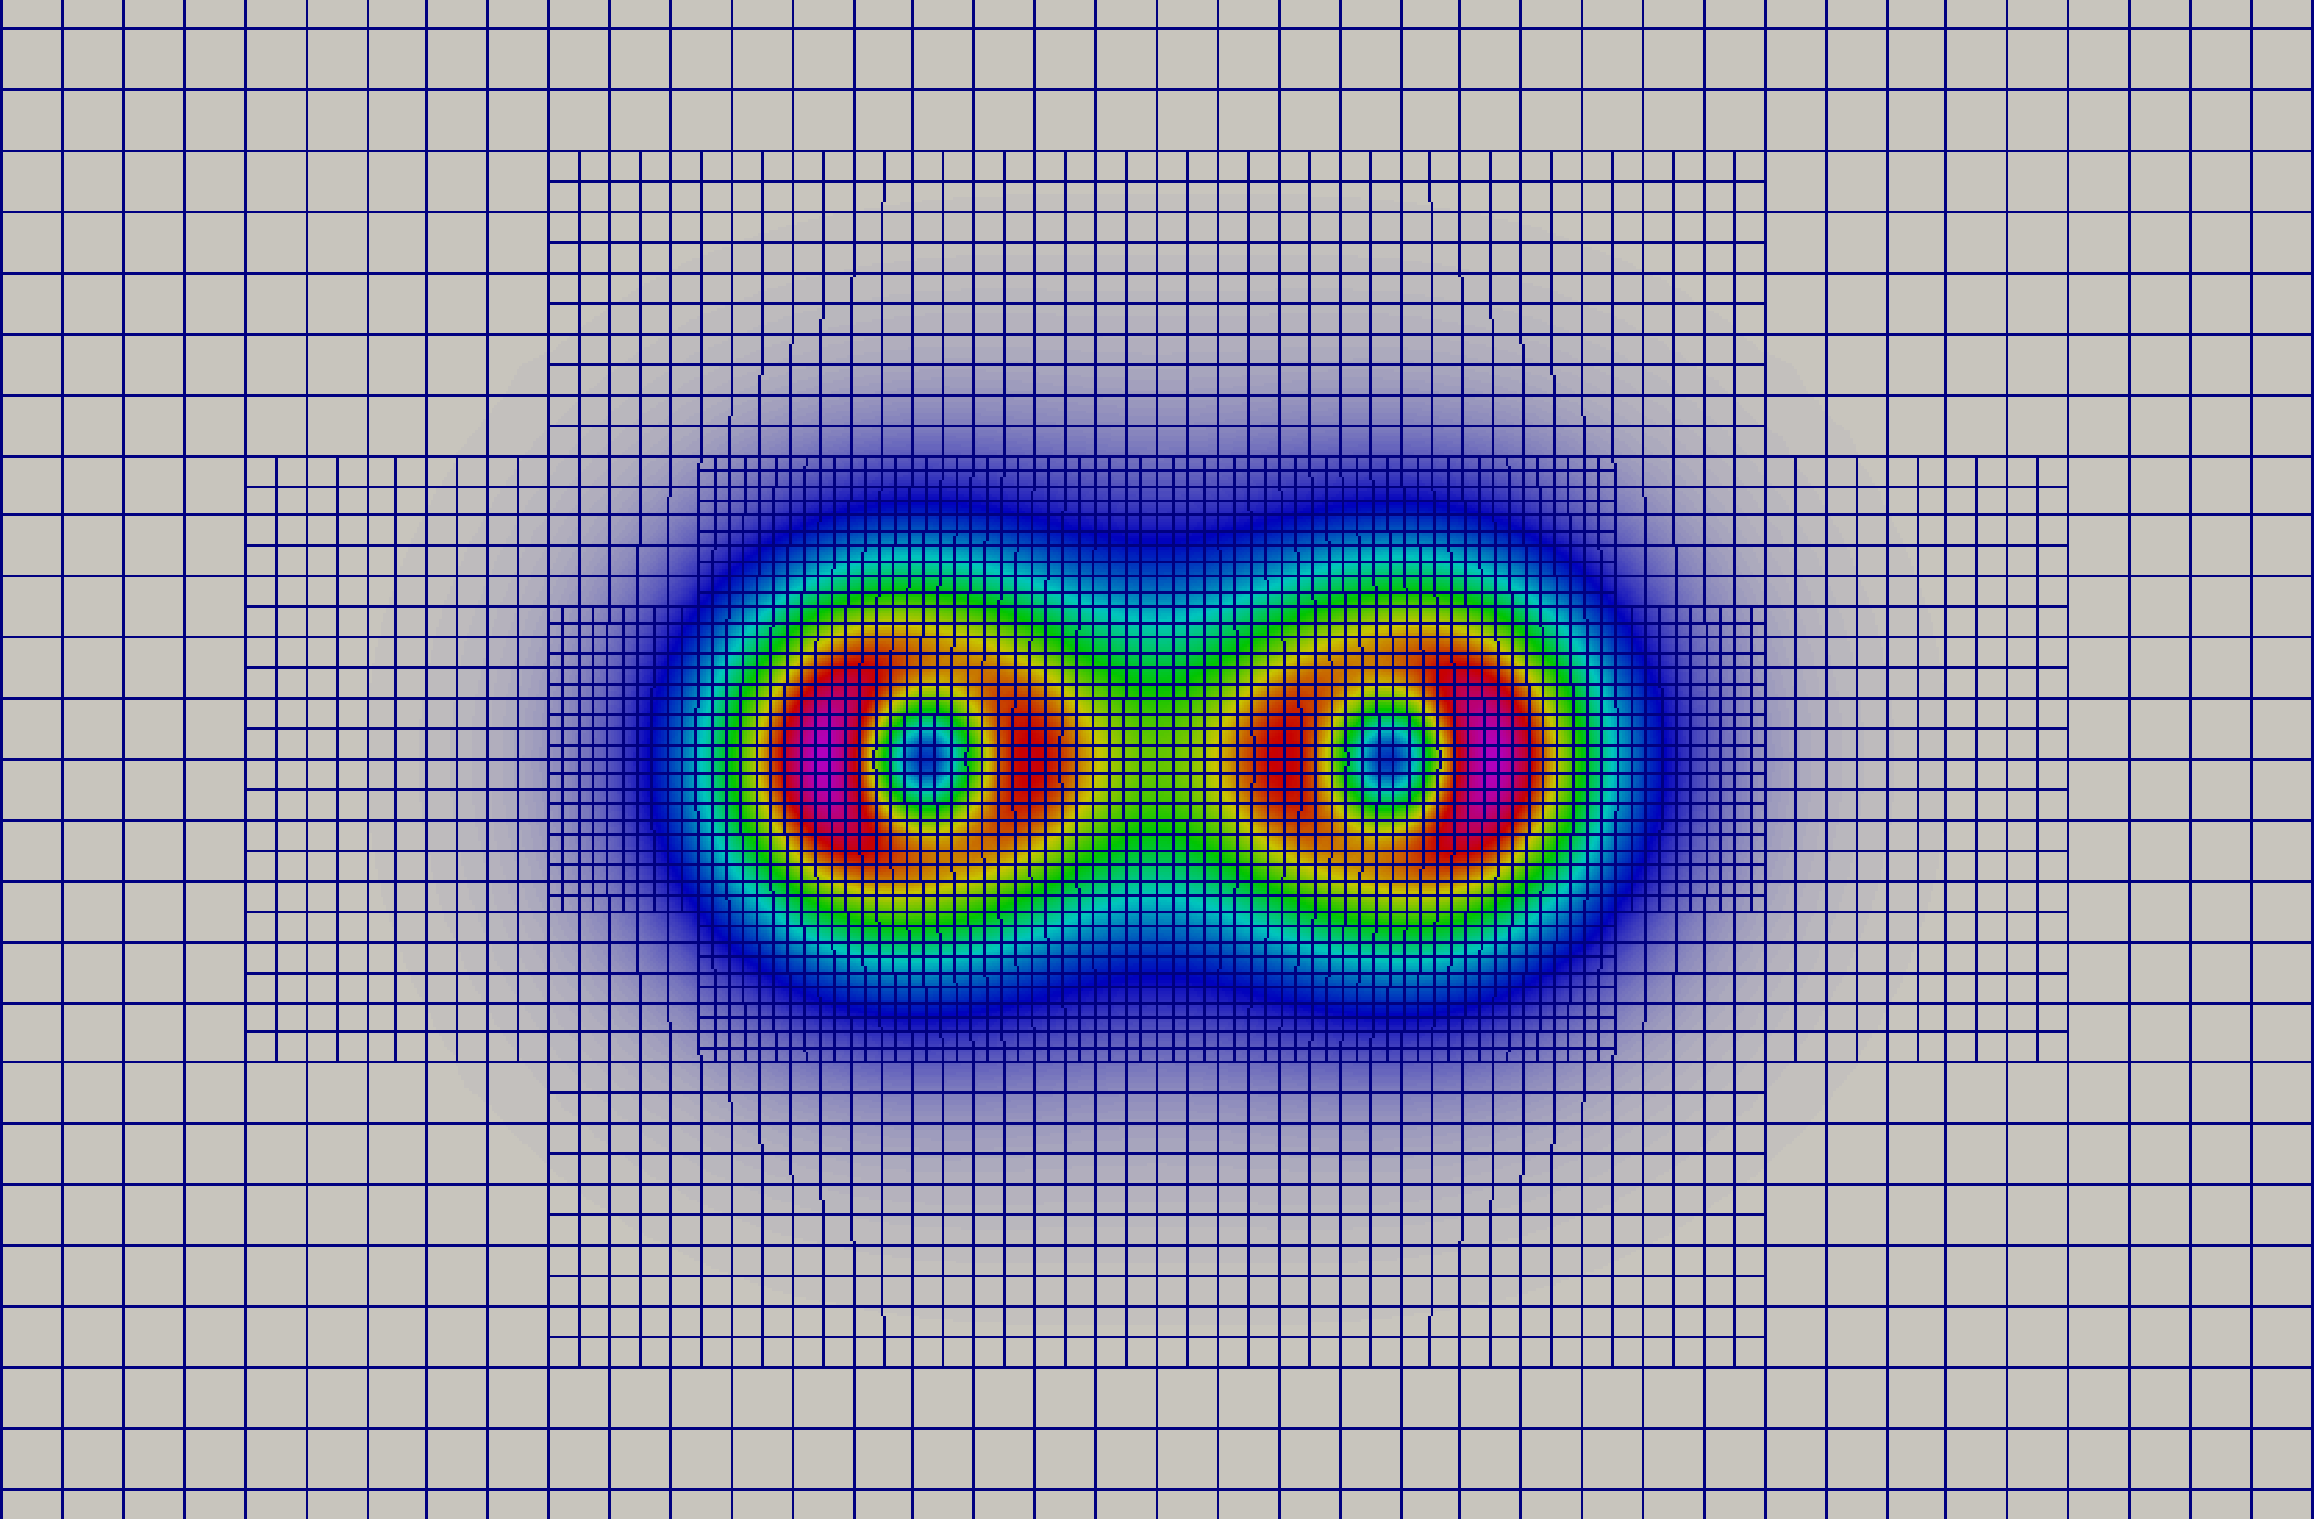
\includegraphics[scale=0.35]{N2.png}
% FILL: image file name
% e.g. cover_image.png
%{contour_5x5x5.pdf}
%{SiCTriplet0000.png}
\hspace{5em}
\end{center}
\end{textblock*}

%USER MANUAL%
\color{dark_grey}
\vspace{1.0em}
\hfill{\Huge \fontfamily{\sfdefault}\selectfont User Manual \\
\raggedleft \huge \fontfamily{\sfdefault}\selectfont Version
% keep the following line as is so that we can replace this using a script:
1.1.0-pre (dev) %VERSION-INFO%
\\\large(generated \today)\\
\vspace{1.5em}
{\Large Sambit Das\,\\Vikram Gavini\,\\Phani Motamarri\\}
\vspace{1.0em}
\large
\noindent with contributions by: \\
    {\Large Krishnendu Ghosh\\}
\vspace{1.0em}
}
%WEBSITE%
\null
\vspace{17em}

{\noindent
{\fontfamily{\sfdefault}\selectfont \href{https://sites.google.com/umich.edu/dftfe}{website of dftfe}}
}

%\begin{textblock*}{0in}(5.25in,-0.8in)
%
\includegraphics[height=0.8in]{CoE-vert.png}
%\end{textblock*}

%LINE%
{\noindent
\color{dark_grey}
\rule{\textwidth}{2pt}
}

}
Copyright (c) 2017-2021 The Regents of the University of Michigan and \hyperref[sec:authors]{DFT-FE authors}.
\pagebreak
\pagenumbering{arabic}

%%%%%%%%%%%%%%%%%%%%%%%%%%%%%%
%%%   END OF DFT-FE MANUAL COVER TEMPLATE    %%%
%%%%%%%%%%%%%%%%%%%%%%%%%%%%%%

\pagebreak

\tableofcontents

\pagebreak

\section{Introduction}
\label{sec:intro}
\dftfe{} is a C++ code for materials modeling from first principles using Kohn-Sham density functional theory.
It is based on adaptive finite-element discretization that handles all-electron and pseudopotential calculations in the 
same framework, and incorporates scalable and efficient solvers for the solution of the Kohn-Sham equations. Importantly, \dftfe{} can handle general geometries and boundary conditions, including periodic, semi-periodic and non-periodic systems. \dftfe{} code builds on top of the deal.II library for everything 
that has to do with finite elements, geometries, meshes, etc., and, through deal.II on p4est for parallel adaptive mesh handling.

\subsection{Authors}
\label{sec:authors}
\dftfe{} is hosted by the \href{http://www-personal.umich.edu/~vikramg/}{Computational Materials Physics
group at University of Michigan}, with Vikram Gavini, Associate Professor of Mechanical Engineering and Materials Science and Engineering, as
the principal investigator broadly overseeing this effort. The code is maintained by a group of principal developers, 
who manage the architecture of the code and the core functionalities. Developers with
significant contributions to core functionalities and code architecture in the past who are 
no longer active principal developers, are listed under principal developers emeriti. 
A subset of the principal developers and mentors are administrators. Finally, all contributors who have
contributed to major parts of the DFT-FE code or sent important fixes and enhancements are listed
under contributors. All the underlying lists are in alphabetical order. 

\paragraph{Principal developers}
\begin{itemize}
	\item Sambit Das (University of Michigan, USA).
	\item Phani Motamarri (University of Michigan, USA).
\end{itemize}

\paragraph{Principal developers emeriti}
\begin{itemize}
	\item Krishnendu Ghosh (University of Michigan, USA).
	\item Shiva Rudraraju (University of Wisconsin Madison, USA).	
\end{itemize}

\paragraph{Contributors}
\begin{itemize}
	\item Sambit Das (University of Michigan, USA).
	\item Denis Davydov (University of Erlangen-Nuremberg, Germany).
	\item Krishnendu Ghosh (University of Michigan, USA).
	\item Phani Motamarri (University of Michigan, USA).
	\item Shiva Rudraraju (University of Wisconsin Madison, USA).
	\item Shukan Parekh (University of Michigan, USA). 	
\end{itemize}

\paragraph{Mentors}
\begin{itemize}
	\item Vikram Gavini (University of Michigan, USA).
\end{itemize}

\subsection{Acknowledgments}
The development of \dftfe{} open source code relating to pseudopotential calculations has been funded in part by the Department of Energy PRISMS Software Center at University of Michigan, and the Toyota Research Institute. The development of \dftfe{} open source code relating to all-electron calculations has been funded by the Department of Energy Basic Energy Science. The methods and algorithms that have been implemented in \dftfe{} are outputs from research activities over many years that have been supported by the Army Research Office, Air Force Office of Scientific Research, Department of Energy Basic Energy Science, National Science Foundation and Toyota Research Institute. 

\subsection{Referencing \dftfe{}}
Please refer to \href{https://sites.google.com/umich.edu/dftfe/referencing}{referencing  \dftfe{}} to properly cite the use of \dftfe{} in your scientific work. 


\section{Useful background information}
\label{sec:background}
We refer to the following articles for a background of the methods and algorithms implemented in \dftfe. \\

\noindent 1. P. Motamarri, M.R. Nowak, K. Leiter , J. Knap, V. Gavini, Higher-order adaptive finite-element methods for Kohn-Sham density functional theory, \emph{J. Comput. Phys.} 253, 308-343 (2013).\\
 
 \noindent 2. P. Motamarri, V. Gavini, Subquadratic-scaling subspace projection method for large-scale Kohn-Sham DFT calculations using spectral finite-element discretization, \emph{Phys. Rev. B} 90, 115127 (2014).\\

\noindent 3. P. Motamarri, V. Gavini,  Configurational forces in electronic structure calculations using Kohn-Sham density functional theory, \emph{Phys. Rev. B} 97 165132 (2018).\\

\noindent In addition, below are some useful references on finite element method and some online resources that provide a background of finite elements and their application to the solution of partial differential equations.\\

\noindent 1. T.J.R. Hughes, The finite element method: linear static and dynamic finite element analysis, Dover Publication, 2000.\\

\noindent 2. K.-J. Bathe, Finite element procedures, Klaus-J\"{u}rgen Bathe, 2014.\\

\noindent 3. The finite element method for problems in physics, online course by Krishna Garikipati. \href{https://www.coursera.org/learn/finite-element-method}{Link}\\

\noindent 4. Online lectures on ``Finite element methods in scientific computing" by Wolfgang Bangerth. \href{http://www.math.colostate.edu/~bangerth/videos.html}{Link}\\ 



\section{Installation}
\label{sec:installation}
All the underlying installation instructions assume a Linux operating system. We assume standard tools and libraries like CMake, compilers- (C, C++ and Fortran), CUDA/HIP (in case of GPU architectures), MPI, and math(BLAS-LAPACK) libraries are pre-installed. Most high-performance computers would have the latest version of these libraries in the default environment. However, in many cases you would have to use \href{http://modules.sourceforge.net/}{Environment Modules} to set the correct environment variables for the above and compilation tools like \href{http://www.cmake.org/}{CMake}. For example, on one of the high-performance computers (UMICH Greatlakes) we develop and test the \dftfe{} code, we can use the following commands to set the desired environment variables
\begin{verbatim}
$ module load cmake/3.18.2
$ module load gcc/8.2.0
$ module load openmpi/3.1.4
$ module load mkl/2018.0.4
$ module load cuda/11.0.2 (if installing for NVIDIA GPUs)
$ module load rocm/5.1.0 (if installing for AMD GPUs)
\end{verbatim}
%In the above mpilibrary denotes the MPI library you are using in your system(for eg: openmpi, mpich or intel-mpi). 
Note the above are shown only as an example. We strongly recommend using the latest stable version of compilers-(C, C++ and Fortran), CUDA/HIP, MPI and math libraries available on your high-performance computer. DFT-FE's installation requires also the following minimum versions of the above compilers and libraries:
\begin{itemize}
    \item CMake 3.17.0
    \item GCC 8.2.0
    \item CUDA 11.0.2/ ROCm (if installing for NVIDIA / AMD GPUs)
\end{itemize}
\textcolor{red}{\bf We currently do not support Intel compilers due to a compilation issue of the deal.II library. Please use GNU compilers only.} Further, if version of CMake greater than 3.17.0 is not available on your machine please install latest version from here \href{http://www.cmake.org/}{CMake} or use pre-installed binaries most appropriate for your machine.

\subsection{Compiling and installing external libraries}
\dftfe{} is primarily based on the open source finite element library \href{http://www.dealii.org/}{deal.II}, through which external dependencies
on \href{http://p4est.org/}{p4est}, \href{http://www.netlib.org/scalapack/}{ScaLAPACK} and BLAS-LAPACK are set. The other required external libraries, which are
not interfaced via deal.II are \href{http://www.alglib.net/}{ALGLIB}, \href{http://www.tddft.org/programs/libxc/}{Libxc}, \href{https://atztogo.github.io/spglib/}{spglib}, \href{http://www.xmlsoft.org/}{Libxml2} and \href{https://elpa.mpcdf.mpg.de/}{ELPA}. DFT-FE also optionally links to \href{https://www.mcs.anl.gov/petsc/}{PETSc} (via deali.II), \href{http://slepc.upv.es/}{SLEPc} (via deali.II) and to \href{https://developer.nvidia.com/nccl}{nccl} (for GPU compilation). The optional dependencies of PETSc and SLEPc are only required for all-electron calculations using DFT-FE, which uses the more stable Gram-Schmidt orthogonalization routine instead of the default Cholesky-Gram-Schmidt orthognalization. For pseudopotential calculations, PETSc and SLEPc dependencies are not required as the default Cholesky-Gram-Schmidt orthogonalization is very robust. \dftfe{} can also be linked to \href{https://github.com/awvwgk/simple-dftd3}{simple-dftd3} and \href{https://github.com/dftd4/dftd4}{dftd4} in order to provide support for the dftd family of dispersion corrections by Grimme et. al.. Below, we give brief installation instructions for each of the above libraries.
\subsubsection{Instructions for dependencies: ALGLIB, Libxc, spglib, Libxml2, ScaLAPACK, ELPA, p4est and nccl (nccl is optional)}
\begin{enumerate}
	\item   {\bf ALGLIB}: Used by \dftfe{} for spline fitting for various radial data. Download the current release of the Alglib free C++ edition from \url{http://www.alglib.net/download.php}. After downloading and unpacking, go to \verb|cpp/src|, and create a shared library using a C++ compiler. For example, using GCC compiler do
\begin{verbatim}
$ g++ -c -fPIC -O2 *.cpp
$ g++ *.o -shared -o libAlglib.so
\end{verbatim}
\item {\bf Libxc}: Used by \dftfe{} for exchange-correlation functionals. Download the current release from \url{http://www.tddft.org/programs/libxc/download/}, and do 
\begin{verbatim}
$ ./configure --prefix=libxc_install_dir_path
              CC=c_compiler CXX=c++_compiler FC=fortran_compiler
	       CFLAGS="-O2 -fPIC" FCFLAGS="-O2 -fPIC" CXXFLAGS="-O2 -fPIC"
     
$ make
$ make install
\end{verbatim}
Do not forget to replace \verb|libxc_install_dir_path| by some appropriate path on your file system and make sure that you have write permissions. Also replace \verb|c_compiler, c++_compiler| and \verb|fortran_compiler| with compilers on your system.

\item {\bf spglib}: Used by \dftfe{} to find crystal symmetries. To install spglib, first obtain the development version of spglib from their github repository by
\begin{verbatim}
$ git clone https://github.com/atztogo/spglib.git	
\end{verbatim}	
and next follow the ``Compiling using cmake'' installation procedure described in \url{https://atztogo.github.io/spglib/install.html}.   	
We recommend using the ccmake gui interface for the installation and also use appropriate compiler for \verb|CMAKE_C_COMPILER|.

\item {\bf Libxml2}: Libxml2 is used by \dftfe{} to read \verb|.xml| files. Most likely, Libxml2 might be already installed in the high-performance computer you are working with. It is usually installed in the default locations like \verb|/usr/lib64| (library path which contains \verb|.so| file for Libxml2, something like \verb|libxml2.so.2|) and \verb|/usr/include/libxml2| (include path). 

Libxml2 can also be installed by doing (Do not use these instructions if you have already have Libxml2 on your system)
\begin{verbatim}
$ git clone https://gitlab.gnome.org/GNOME/libxml2.git
$ ./autogen.sh --prefix=Libxml_install_dir_path
$ make
$ make install 
\end{verbatim}
There might be errors complaining that it can not create regular file libxml2.py in /usr/lib/python2.7/site-packages, but that should not matter.

\item {\bf ScaLAPACK}: ScaLAPACK library is used by DFT-FE via deal.II for its parallel linear algebra routines involving dense matrices, as well being a dependency for ELPA. \textcolor{red}{\bf If Intel MKL math library is available, please skip this step, as the ScaLAPACK libraries therein can be used directly.} If Intel MKL math library is not available, Netlib ScaLAPACK \url{http://www.netlib.org/scalapack/} needs to be installed using the instructions below. Download the current release version (2.2.0) from \url{http://www.netlib.org/scalapack/#\_software}, and build a shared library (use \verb|BUILD_SHARED_LIBS=ON|, \verb|BUILD_STATIC_LIBS=OFF| and \verb|BUILD_TESTING=OFF|) installation of ScaLAPACK using cmake. We recommend using the ccmake gui interface for the installation.  Further, use the appropriate compilers for \verb|CMAKE_C_COMPILER| and \verb|CMAKE_FORTRAN_COMPILER|, and also use \verb|-fPIC| flag for \verb|CMAKE_C_FLAGS| and \verb|CMAKE_Fortran_FLAGS|. For best performance, ScaLAPACK must be linked to optimized BLAS-LAPACK libraries by using\\ \verb|USE_OPTIMIZED_LAPACK_BLAS=ON|, and providing external paths to BLAS-LAPACK libraries (MKL, OpenBlas, ESSL etc.) during the cmake configuration. 
%Alternatively one can also use the python based installer~\url{http://www.netlib.org/scalapack/scalapack_installer.tgz} for Linux.

\item {\bf ELPA}: ELPA library is used by DFT-FE for its parallel linear algebra routines involving dense matrices. ELPA requires the ScaLAPACK library (see above) as a dependency. Download the latest version elpa-2022.11.001 from \url{https://elpa.mpcdf.mpg.de/software/} and follow the installation instructions in there. Example of ELPA installation on UMICH Greatlakes supercomputer with GNU compiler, Open MPI library, and Intel MKL math library:
\begin{verbatim}
$ cd elpaDir
$ mkdir build
$ cd build
$ ../configure --enable-openmp FC=mpif90 CC=mpicc CXX=mpicxx 
FCFLAGS="-fopenmp -O2 -march=native" CFLAGS="-fopenmp -O2 -march=native" 
CXXFLAGS="-fopenmp -O2 -march=native" --prefix=elpa_install_path
SCALAPACK_LDFLAGS=" -L${MKLROOT}/lib/intel64 -lmkl_scalapack_lp64
-Wl,--no-as-needed -lmkl_intel_lp64
-lmkl_gnu_thread -lmkl_core -lmkl_blacs_openmpi_lp64 -lgomp -lpthread -lm -ldl" 
SCALAPACK_FCFLAGS="-L${MKLROOT}/lib/intel64 -lmkl_scalapack_lp64
-Wl,--no-as-needed -lmkl_gf_lp64 -lmkl_gnu_thread -lmkl_core
-lmkl_blacs_openmpi_lp64 -lgomp -lpthread -lm -ldl"
$ make -j 4
$ make install
\end{verbatim}
The MKL paths and linker flags were obtained with the help of \href{https://software.intel.com/en-us/articles/intel-mkl-link-line-advisor}{Intel MKL Link Line Advisor} for GNU Fortran compiler (Note the usage of \verb|-lmkl_gf_lp64| flag above).\\ 

If the machine of interest has NVIDIA/AMD GPUs and CUDA/ROCm compiler, ELPA can take advantage of GPUs. For example on OLCF Summit GPU nodes, we use the following configure line
\begin{verbatim}
../configure CXX=mpic++ FC=mpif90 CC=mpicc 
CXXFLAGS="-O2 -fPIC -mcpu=power9 -mvsx -maltivec"
FCFLAGS="-O2 -fPIC -mcpu=power9 -mvsx -maltivec" 
CFLAGS="-O2 -fPIC -mcpu=power9 -mvsx -maltivec"
--enable-nvidia-gpu --with-NVIDIA-GPU-compute-capability="sm_70" 
--enable-gpu-streams=nvidia --with-cuda-path="$OLCF_CUDA_ROOT"
--with-cuda-sdk-path="$OLCF_CUDA_ROOT" 
--prefix=elpa_install_path 
LDFLAGS="-L$scalapack_lib_path -lscalapack  
-L$OLCF_ESSL_ROOT/lib64 -lessl 
-L$OLCF_NETLIB_LAPACK_ROOT/lib64 -llapack 
-L$OLCF_OPENBLAS_ROOT/lib -lopenblas"
--disable-sse --disable-sse-assembly --disable-avx 
--disable-avx2 --disable-avx512 --enable-c-tests=no --enable-cpp-tests=no
--enable-option-checking=fatal --enable-shared 
\end{verbatim}


We provice another ELPA installation example on OLCF Crusher nodes with AMD GPUs and ROCm compiler:
\begin{verbatim}
../configure CXX=hipcc CC=hipcc FC=ftn 
FCFLAGS="-march=znver3 -O2 -fPIC" 
CFLAGS="-march=znver3 -fPIC -O2 -I${ROCM_PATH}/include 
-I${ROCM_PATH}/hip/include -I${ROCM_PATH}/hipcub/include
-I${ROCM_PATH}/rocblas/include  --amdgpu-target=gfx90a
-I${MPICH_DIR}/include" CXXFLAGS="-march=znver3 -std=c++14 
-I${ROCM_PATH}/include -fPIC -O2 -I${ROCM_PATH}/hip/include 
-I${ROCM_PATH}/hipcub/include -I${ROCM_PATH}/rocblas/include 
--amdgpu-target=gfx90a -I${MPICH_DIR}/include" --enable-amd-gpu
--enable-gpu-streams=amd --prefix=elpa_install_path
LIBS="-L${ROCM_PATH}/lib -lamdhip64 -L${ROCM_PATH}/rocblas/lib 
-lrocblas -L${MPICH_DIR}/lib -lmpi -L${CRAY_MPICH_ROOTDIR}/gtl/lib -lmpi_gtl_hsa 
-L$scalapack_lib_path -lscalapack
-L/sw/crusher/spack-envs/base/opt/cray-sles15-zen3/gcc-11.2.0/openblas-0.3.17-fip547hyhcrii2xgj5rmge3oyxgnfhkp/lib -lopenblas 
-L$netlib_lapack_lib_path -llapack" 
--disable-sse --disable-sse-assembly --disable-avx --disable-avx2 
--disable-avx512 --enable-c-tests=no --enable-option-checking=fatal
--enable-shared --enable-cpp-tests=no --enable-hipcub
\end{verbatim}


Note the use of LDFLAGS instead of SCALAPACK\_LDFLAGS and SCALAPACK\_FCFLAGS, since we are using netlib ScaLAPACK instead of Intel MKL ScaLAPACK in the above. Also note use of
\begin{verbatim}
    --disable-sse --disable-sse-assembly --disable-avx --disable-avx2 --disable-avx512
\end{verbatim} 
above. \textcolor{red}{\bf Some or all of these options may be required for systems without Intel CPUs such as IBM Power and AMD Epyc processors depending on what they support.} Finally, we remark that to avoid errors during ELPA configuration step, please export the library paths of ScaLAPACK and blas libraries, for example:
\begin{verbatim}
export LD_LIBRARY_PATH=$LD_LIBRARY_PATH:$blas_lib_path

export LD_LIBRARY_PATH=$LD_LIBRARY_PATH:$netlib_lapack_lib_path

export LD_LIBRARY_PATH=
$LD_LIBRARY_PATH:$ROCM_PATH/lib:$ROCM_PATH/hip/lib:$ROCM_PATH/lib:$ROCM_PATH/rocblas/lib
\end{verbatim}

\item   {\bf p4est}: This library is used by deal.II to create and distribute finite-element meshes across multiple processors. Download the v2.2 tarball of p4est from \url{http://www.p4est.org/}. Next download the \verb|p4est-setup.sh| script from \url{https://raw.githubusercontent.com/dftfeDevelopers/dftfe/manual/p4est-setup.sh}. Use the script to automatically compile and install a debug and optimized version of p4est by doing
\begin{verbatim}
$ chmod u+x p4est-setup.sh
$ ./p4est-setup.sh p4est-x-y-z.tar.gz p4est_install_dir_path
\end{verbatim}

%Also download the script from \url{https://github.com/dftfeDevelopers/dftfe/raw/manual/p4est-setup.sh} if using Intel compilers, or from \url{https://dealii.org/developer/external-libs/p4est.html} if using GCC compilers. Use the script to automatically compile and install a debug and optimized version of p4est by doing

\item {\bf nccl/rccl (optional)}: nccl (CUDA) and rccl (ROCm) libraries are optional dependency for DFT-FE for optimal GPU Direct MPI collective communication calls. This library is recommended for running very large system sizes (greater than 20,000 electrons) on GPUs using DFT-FE. Caution: nccl/rccl library requires appropriate hardware support for GPU Direct MPI communication and GPU Aware MPI library. To install nccl/rccl, use the appropriate release version (corresponding to the CUDA/ROCm compiler version) from \url{https://github.com/NVIDIA/nccl} (CUDA) \url{https://github.com/ROCmSoftwarePlatform/rccl} (ROCm) and follow installation instructions therein.

\end{enumerate}


\subsubsection{Instructions for deal.II}
Assuming the above dependencies (p4est and ScaLAPACK) are installed, we now briefly discuss the steps to compile and install deal.II library linked with the above dependencies. You need to install two variants of the deal.II library-- one variant linked with real scalar type PETSc and SLEPc installations, and the other variant linked with complex scalar type PETSc and SLEPc installations. 

\begin{enumerate}

\item Obtain the customized version of deal.II library via
\begin{verbatim}
$ git clone -b dealiiCustomizedCUDARelease https://github.com/dftfeDevelopers/dealii.git
\end{verbatim}

\item In addition to requiring C, C++ and Fortran compilers, MPI library, and CMake, deal.II additionally requires BOOST library. If not found externally, cmake will resort to the bundled BOOST that comes along with deal.II. Based on our experience, we recommend to use the deal.II's bundled boost (enforced by unsetting/unloading external BOOST library environment paths) to avoid compilation issues. Please do not install deal.II with GPU support as that is not needed by DFT-FE. Further, when installing deal.II for (DFT-FE with GPU support), one must use \verb|-DDEAL_II_ALLOW_PLATFORM_INTROSPECTION=OFF| to avoid compilation failure of DFT-FE.

\item
\begin{verbatim}
$ mkdir build
$ cd build
$ cmake -DCMAKE_INSTALL_PREFIX=dealii_install_dir_path
        otherCmakeOptions ../deal.II
$ make -j 8        
$ make install
\end{verbatim}
{\bf ``otherCmakeOptions'' include} the following options for CPU installation:
\begin{verbatim}
-DCMAKE_CXX_STANDARD=14
-DCMAKE_C_COMPILER=c_compiler
-DCMAKE_CXX_COMPILER=cxx_compiler
-DCMAKE_Fortran_COMPILER=fortran_compiler
-DMPI_C_COMPILER=mpi_c_compiler_wrapper
-DMPI_CXX_COMPILER=mpi_cxx_compiler_wrapper
-DMPI_Fortran_COMPILER=mpi_fortran_compiler_wrapper
-DCMAKE_CXX_FLAGS=cxx_flags
-DCMAKE_C_FLAGS=c_flags
-DDEAL_II_WITH_MPI=ON -DDEAL_II_WITH_64BIT_INDICES=ON
-DDEAL_II_WITH_P4EST=ON -DP4EST_DIR=p4est_install_dir_path
-DDEAL_II_WITH_LAPACK=ON
-DLAPACK_DIR=lapack_dir_paths (both BLAS and LAPACK directory paths)
-DLAPACK_FOUND=true
-DLAPACK_LIBRARIES=lapack_lib_paths (both BLAS and LAPACK library paths)
-DDEAL_II_WITH_SCALAPACK=ON
-DSCALAPACK_DIR=scalapack_dir_path (only required if linking to netlib ScaLAPACK)
-DSCALAPACK_LIBRARIES=scalapack_lib_path
-DDEAL_II_WITH_TBB=OFF
-DDEAL_II_WITH_TASKFLOW=OFF
-DDEAL_II_COMPONENT_EXAMPLES=OFF
\end{verbatim}



\end{enumerate}	
 For more information about installing deal.II library refer to \url{https://dealii.org/developer/readme.html}. We also provide here an example of deal.II installation, which we did on UMICH Greatlakes supercomputer with GNU compiler, Open MPI library, and Intel MKL math library
\begin{verbatim}
$ mkdir build
$ cd build
$ cmake
-DCMAKE_CXX_STANDARD=14
-DCMAKE_C_COMPILER=gcc 
-DCMAKE_CXX_COMPILER=g++
-DCMAKE_Fortran_COMPILER=gfortran
-DMPI_C_COMPILER=mpicc 
-DMPI_CXX_COMPILER=mpicxx 
-DMPI_Fortran_COMPILER=mpif90
-DCMAKE_CXX_FLAGS="-march=native -std=c++14"
-DCMAKE_C_FLAGS="-march=native -std=c++14"
-DDEAL_II_CXX_FLAGS_RELEASE="-O2"
-DDEAL_II_COMPONENT_EXAMPLES=OFF
-DDEAL_II_WITH_MPI=ON
-DDEAL_II_WITH_64BIT_INDICES=ON
-DDEAL_II_WITH_TBB=OFF
-DDEAL_II_WITH_TASKFLOW=OFF 
-DDEAL_II_WITH_P4EST=ON 
-DP4EST_DIR=p4est_install_path 
-DDEAL_II_WITH_LAPACK=ON -DLAPACK_DIR="${MKLROOT}/lib/intel64"
-DLAPACK_FOUND=true
-DLAPACK_LIBRARIES="-L${MKLROOT}/lib/intel64
-Wl,--no-as-needed -lmkl_intel_lp64
-lmkl_gnu_thread -lmkl_core -lgomp -lpthread -lm
-ldl" -DLAPACK_INCLUDE_DIRS="-I${MKLROOT}/include" 
-DDEAL_II_WITH_SCALAPACK=ON
-DSCALAPACK_LIBRARIES="-L${MKLROOT}/lib/intel64
-lmkl_scalapack_lp64 -Wl,--no-as-needed
-lmkl_intel_lp64 -lmkl_gnu_thread -lmkl_core
-lmkl_blacs_openmpi_lp64 -lgomp -lpthread -lm
-ldl"
-DCMAKE_INSTALL_PREFIX=dealii_install_path ../dealii
$ make -j 8
$ make install
\end{verbatim}
The values for \verb|-DLAPACK_DIR|,\verb|-DLAPACK_LIBRARIES| and \verb|-DLAPACK_LINKER_FLAGS| were obtained with the help of \href{https://software.intel.com/en-us/articles/intel-mkl-link-line-advisor}{Intel MKL Link Line Advisor} for GNU C++ compiler (cf. Fig.~\ref{fig:intelmkl}).\\ 
\begin{figure}[htp]
    \centering
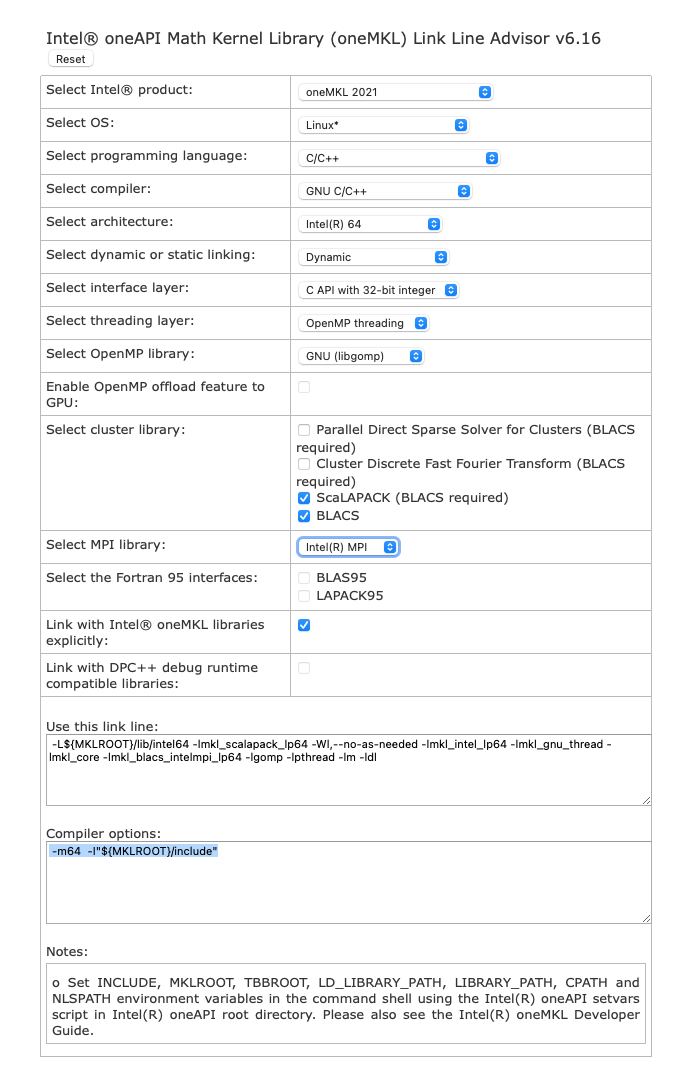
\includegraphics[scale=0.4]{intelmklLineAdvisorExampleNew.png}
    \caption{Example usage of Intel MKL line advisor. Use the options in the ``link line'' generated by the line advisor tool. Please note to change ``intelmpi'' in ``-lmkl\_blacs\_intelmpi\_lp64'' to ``openmpi'' if using openmpi MPI library.}
    \label{fig:intelmkl}
\end{figure}

%Note that in the above procedure one is installing the development version of deal.II library and this version is continuously updated by deal.II developers, which can sometimes lead to installation issues on certain compilers. If you face any issues during the installation procedure of deal.II development version as explained above, you may alternatively obtain the current release version of deal.II by downloading and unpacking the .tar.gz file from \url{https://www.dealii.org/download.html} and following the same procedure as above. If you still face installation issues, and/or if you have any questions about the deal.II installation, please contact the deal.II developers at \href{https://groups.google.com/d/forum/dealii}{deal.II mailing lists}.\\

{\bf Using AVX, AVX-512 instructions in deal.II:}\\
deal.II compilation will automatically try to pick the available vector instructions on the sytem like SSE2, AVX and AVX-512, and generate the following output message during compilation   
\begin{verbatim}
-- Performing Test DEAL_II_HAVE_SSE2
-- Performing Test DEAL_II_HAVE_SSE2 - Success/Failed
-- Performing Test DEAL_II_HAVE_AVX
-- Performing Test DEAL_II_HAVE_AVX - Success/Failed
-- Performing Test DEAL_II_HAVE_AVX512
-- Performing Test DEAL_II_HAVE_AVX512 - Success/Failed
-- Performing Test DEAL_II_HAVE_OPENMP_SIMD
-- Performing Test DEAL_II_HAVE_OPENMP_SIMD - Success/Failed
\end{verbatim}
``Success'', means deal.II was able to use the corresponding vector instructions, and ``Failed'' would mean otherwise. If deal.II is not able to pick an available vector instruction on your high-performance computer, please contact the deal.II developers at \href{https://groups.google.com/d/forum/dealii}{deal.II mailing lists} and/or contact your high-performance computer support for guidance on how to use the correct compiler flags for AVX or AVX-512. 

Ensure that deal.II picks up AVX-512, which is strongly recommended for obtaining maximum performance on the new Intel Xeon Phi (KNL) and Skylake processors, both of which support Intel AVX-512 instructions.

\subsubsection{Instructions for simple-dftd3 and dftd4}

\begin{enumerate}
	\item   {\bf simple-dftd3}: Used by \dftfe{} to provide dftd3 corrections to energy, force and stress. Download the current release (0.6.0 at the time of writing) of simple-dftd3 from \url{https://github.com/awvwgk/simple-dftd3/releases}. After downloading and unpacking, use cmake to build the library. For example, using GNU compiler and Intel MKL for BLAS, do
\begin{verbatim}
$ FC=gfortran cmake -B _build 
-DBLAS_LIBRARIES="-L${MKLROOT}/lib/intel64 
-Wl,--no-as-needed -lmkl_gf_lp64 
-lmkl_gnu_thread -lmkl_core -lgomp 
-lpthread -lm -ldl" 
-DCMAKE_INSTALL_PREFIX=simple_dftd3_install_path
$ cmake --build _build
$ cmake --install _build 
\end{verbatim}
	\item   {\bf dftd4}: Used by \dftfe{} to provide dftd4 corrections to energy, force and stress. Download the current release (3.4.0 at the time of writing) of dftd4 from \url{https://github.com/dftd4/dftd4/releases}. After downloading and unpacking, use cmake to build the library. For example, using GNU compiler and Intel MKL for BLAS and LAPACK, do
\begin{verbatim}
$ FC=gfortran cmake -B _build 
-DBLAS_LIBRARIES="-L${MKLROOT}/lib/intel64 
-Wl,--no-as-needed -lmkl_gf_lp64 
-lmkl_gnu_thread -lmkl_core -lgomp 
-lpthread -lm -ldl" 
-DLAPACK_LIBRARIES="-L${MKLROOT}/lib/intel64 
-Wl,--no-as-needed -lmkl_gf_lp64 
-lmkl_gnu_thread -lmkl_core -lgomp 
-lpthread -lm -ldl" 
-DCMAKE_INSTALL_PREFIX=dftd4_install_path
$ cmake --build _build
$ cmake --install _build 
\end{verbatim}
\end{enumerate}
The values for \verb|-DBLAS_LIBRARIES| and \verb|-DLAPACK_LIBRARIES| were obtained with the help of \href{https://software.intel.com/en-us/articles/intel-mkl-link-line-advisor}{Intel MKL Link Line Advisor} for GNU fortran compiler.\\ 

\subsection{Obtaining and Compiling \dftfe{}}\label{sec:dftfeinstall}
Assuming that you have already installed the above external dependencies, next follow the steps below to obtain and compile \dftfe{}.
\begin{enumerate}
\item Obtain the source code of the current release of \dftfe{} with all current patches using \href{https://git-scm.com/}{Git}:
\begin{verbatim}
$ git clone -b release1.0 https://github.com/dftfeDevelopers/dftfe.git
$ cd dftfe
\end{verbatim}
Do \verb|git pull| in the \verb|dftfe| directory any time to obtain new patches that have been added since your \verb|git clone| or last \verb|git pull|.
If you are not familiar with Git, you may download the current release tarball from the \href{https://sites.google.com/umich.edu/dftfe/download}{Downloads} page in our website, but downloading via Git is recommended to avail new patches seamlessly. 


%{\bf Obtaining previous releases:} (Skip this part if you are using the current release version)
%\begin{enumerate}
%\item
%\begin{verbatim}
%$ git clone https://github.com/dftfeDevelopers/dftfe.git 
%$ cd dftfe
%\end{verbatim}

%\item To get the list of all release tags (current and previous releases) do
%\begin{verbatim}
%$ git tag -l
%\end{verbatim}

%\item
%Choose the desired release tag name and do
%\begin{verbatim}
%$ git checkout tags/<tag_name> 
%\end{verbatim}
%\end{enumerate}
%Alternatively, you could download the appropriate tarball from \href{https://github.com/dftfeDevelopers/dftfe/releases}{github-releases}.

\item Set paths to external libraries (deal.II, ALGLIB, Libxc, spglib, Libxml2, and ELPA), C++ compiler, and C++ compiler flags in \verb|setupUser.sh|, which is a script to compile \dftfe~using cmake. nccl library can also be optionally provided in case of GPU compilation. If compiling only for CPUs, set the following to OFF
\begin{verbatim}
withGPU=OFF
withDCCL=OFF
\end{verbatim}
For GPU compilation, \verb|withGPU|, \verb|gpuLang|, and \verb|gpuVendor| should be set \verb|ON|, \verb|"cuda"/"hip"| and \verb|"nvidia"/"amd"| respectively. Also appropriate C++ compiler, device (denoting GPU) compilation and architecture flags must be passed to access CUDA/HIP compiler for device code compilation. \textcolor{red}{\bf CAUTION! GPU enabled DFT-FE compilation must only be run on machines with GPU access.} 
\item To compile \dftfe{}, first create a build directory anywhere on your machine. Next from inside the build directory do
\begin{verbatim}
$ bash $dftfe_source/setupUser.sh
\end{verbatim} 
Please use the full directory path for \verb|$dftfe_source| above. Also note that sometimes compilation on login node can crash due to insufficient memory. In those cases, we recommend using an interactive job if available on your computing cluster.

\item If compilation is successful, the following executables will be created:
\begin{verbatim}
$dftfe_build_dir/release/real/dftfe
$dftfe_build_dir/release/complex/dftfe
\end{verbatim}

\item
To compile \dftfe{} in debug mode (much slower but useful for debugging), set \verb|build_type=Debug| in \verb|setupUser.sh| and do:
\begin{verbatim}
$ bash $dftfe_source/setupUser.h
\end{verbatim}
which will create the following debug mode executables:
\begin{verbatim}
$dftfe_build_dir/debug/real/dftfe
$dftfe_build_dir/debug/complex/dftfe
\end{verbatim}
\end{enumerate}



\subsection{Optional PETSc, SLEPc, deal.II and \dftfe~ installation instructions for all-electron calculations using DFT-FE}
Users can ignore this section if only interested in pseudopotential calculations. The optional dependencies of PETSc and SLEPc are only required for all-electron calculations using DFT-FE, which uses the more stable Gram-Schmidt orthogonalization routine instead of the default Cholesky-Gram-Schmidt orthognalization. 
    
\begin{enumerate}
\item {\bf PETSc}: PETSc is a parallel linear algebra library. \dftfe{} with PETSc and SLEPc dependencies needs two variants of the PETSc installation---one with real scalar type and the another with complex scalar type. Also both the installation variants must have 64-bit indices and optimized mode enabled during the installation. To install PETSc, first download the current release (3.15.0 or later) tarball from \url{https://www.mcs.anl.gov/petsc/download/index.html}, unpack it, and follow the installation instructions in \url{https://www.mcs.anl.gov/petsc/documentation/installation.html}. 
	
Below, we show an example installation for the real scalar type variant. 
This example should be used only as a reference.
\begin{verbatim}
$ ./configure --prefix=petscReal_install_dir_path --with-debugging=no 
              --with-64-bit-indices=true --with-cc=c_compiler
              --with-cxx=c++_compiler --with-fc=fortran_compiler
              --with-blas-lapack-lib=(optimized BLAS-LAPACK library path) 
              CFLAGS=c_compilter_flags CXXFLAGS=c++_compiler_flags
	              FFLAGS=fortran_compiler_flags

$ make PETSC_DIR=prompted by PETSc 
       PETSC_ARCH=prompted by PETSc

$ make PETSC_DIR=prompted by PETSc 
       PETSC_ARCH=prompted by PETSc
       install
\end{verbatim}
For the complex installation variant, unpack a fresh PETSc directory (required) from the tarball and repeat the above steps with the only changes being adding  \verb|--with-scalar-type=complex| and \verb|--with-fortran-kernels=true| to the configuration step (\verb|./configure|) as well as providing a new installation path to \verb|--prefix|. Below we provide example configure lines for real and complex versions on UMICH Greatlakes supercomputer with GNU compiler, Open MPI library, and Intel MKL math library:
\begin{verbatim}
./configure --prefix=petsc_real_install_path --with-debugging=no 
--with-64-bit-indices=true --with-cc=mpicc --with-cxx=mpicxx 
--with-fc=mpif90 --with-blas-lapack-lib="-Wl,--start-group
${MKLROOT}/lib/intel64/libmkl_intel_lp64.a 
${MKLROOT}/lib/intel64/libmkl_gnu_thread.a 
${MKLROOT}/lib/intel64/libmkl_core.a -Wl,--end-group -lgomp -lpthread -lm -ldl"
CFLAGS="-O2" CXXFLAGS="-O2" FFLAGS="-O2"

./configure --prefix=petsc_complex_install_path --with-debugging=no
--with-64-bit-indices=true --with-cc=mpicc --with-cxx=mpicxx
--with-fc=mpif90 --with-fortran-kernels=true --with-scalar-type=complex
--with-blas-lapack-lib="-Wl,--start-group 
${MKLROOT}/lib/intel64/libmkl_intel_lp64.a ${MKLROOT}/lib/intel64/libmkl_gnu_thread.a
${MKLROOT}/lib/intel64/libmkl_core.a -Wl,--end-group -lgomp -lpthread -lm -ldl"
CFLAGS="-O2" CXXFLAGS="-O2" FFLAGS="-O2"
\end{verbatim}

\item {\bf SLEPc}: The SLEPc library is built on top of PETSc, and it is used in DFT-FE for Gram-Schmidt Orthogonalization. To install SLEPc, first download the current release (3.15.0 or later) tarball from \url{http://slepc.upv.es/download/}, and then follow the installation procedure described in \url{http://slepc.upv.es/documentation/instal.htm}. {\bf Important: } SLEPc installation requires PETSc to be installed first. You also need to create two separate SLEPc installations- one for PETSc installed with \\\verb|--with-scalar-type=real|, and the second for PETSc installed with \verb|--with-scalar-type=complex|. 
	
For your reference you provide here an example installation of SLEPc for real scalar type
\begin{verbatim}
$ export PETSC_DIR=petscReal_install_dir_path
$ unset PETSC_ARCH
$ cd downloaded_slepc_dir
$ ./configure --prefix=slepcReal_install_dir_path
$ make
$ make install
\end{verbatim}


\item {\bf deal.II}: Assuming PETSc and SLEPc are installed, we now briefly discuss the steps to compile and install deal.II library linked with the above dependencies. You need to install two variants of the deal.II library---one variant linked with real scalar type PETSc and SLEPc installations, and the other variant linked with complex scalar type PETSc and SLEPc installations. 

\begin{verbatim}
$ mkdir buildReal
$ cd buildReal
$ cmake -DCMAKE_INSTALL_PREFIX=dealii_petscReal_install_dir_path
        otherCmakeOptions ../deal.II
$ make install
\end{verbatim}
{\bf ``otherCmakeOptions'' include} the following options
\begin{verbatim}
-DCMAKE_C_COMPILER=c_compiler
-DCMAKE_CXX_COMPILER=cxx_compiler
-DCMAKE_Fortran_COMPILER=fortran_compiler
-DMPI_C_COMPILER=mpi_c_compiler_wrapper
-DMPI_CXX_COMPILER=mpi_cxx_compiler_wrapper
-DMPI_Fortran_COMPILER=mpi_fortran_compiler_wrapper
-DCMAKE_CXX_FLAGS=cxx_flags
-DCMAKE_C_FLAGS=c_flags
-DDEAL_II_WITH_MPI=ON -DDEAL_II_WITH_64BIT_INDICES=ON
-DDEAL_II_WITH_P4EST=ON -DP4EST_DIR=p4est_install_dir_path
-DDEAL_II_WITH_PETSC=ON -DPETSC_DIR=petscReal_install_dir_path 
-DDEAL_II_WITH_SLEPC=ON -DSLEPC_DIR=slepcReal_install_dir_path
-DDEAL_II_WITH_LAPACK=ON
-DLAPACK_DIR=lapack_dir_path 
-DLAPACK_FOUND=true 
-DLAPACK_LIBRARIES=lapack_lib_path
-DSCALAPACK_DIR=scalapack_dir_path (only required if linking to Netlib ScaLAPACK)
-DSCALAPACK_LIBRARIES=scalapack_lib_path
-DDEAL_II_WITH_TBB=OFF
-DDEAL_II_WITH_TASKFLOW=OFF
-DDEAL_II_COMPONENT_EXAMPLES=OFF
\end{verbatim}

\item {\bf DFT-FE}: Follow the same instructions as in Sec.~\ref{sec:dftfeinstall}, except to modify the \verb|setupUserPetsc.sh| script instead of the \verb|setupUser.sh|. In \verb|setupUserPetsc.sh|, in addition to updating the paths and flags as discussed in Sec~\ref{sec:dftfeinstall}, update the dealii installation paths from the previous step as follows:
\begin{verbatim}
dealiiPetscRealDir=dealii_petscReal_install_dir_path
dealiiPetscComplexDir=dealii_petscComplex_install_dir_path
\end{verbatim}
\end{enumerate}


\subsection{Important generic instructions}
\begin{itemize}
\item We strongly recommend to link to optimized BLAS-LAPACK library. If using Intel MKL for BLAS-LAPACK library, it is {\bf very important} to use \href{https://software.intel.com/en-us/articles/intel-mkl-link-line-advisor}{Intel MKL Link Line Advisor} to correctly link with Intel MKL for installations of PETSc, ScaLAPACK, ELPA, deal.II, and PETSc. To exploit performance benefit from threads, we recommend (strongly recommended for the new Intel Xeon Phi (KNL) and Skylake processors) linking to threaded versions of Intel MKL libraries by using the options ``threading layer'' and  ``OpenMP library'' in \href{https://software.intel.com/en-us/articles/intel-mkl-link-line-advisor}{Intel MKL Link Line Advisor}.

\item Use \verb|-fPIC| compiler flag for compilation of \dftfe{} and its dependencies, to prevent linking errors during \dftfe{} compilation.	

\item \textcolor{red}{\bf CAUTION! It is  highly recommended to compile deal.II, p4est, ScaLAPACK, ELPA, \dftfe, PETSc and SLEPc~ with the same compilers, same BLAS-LAPACK libraries (if applicable), and same MPI libraries. This prevents deal.II compilation issues, occurrence of run time crashes, and \dftfe{} performance degradation.}  
\end{itemize}


\section{Running \dftfe}
\label{sec:run}
After compiling \dftfe{} as described in Section~\ref{sec:installation}, we have now two executables --- \verb|/build/release/real/dftfe| and \verb|/build/release/complex/dftfe|. The \verb|/build/release/real/dftfe| executable, which uses real data-structures is sufficient for fully non-periodic problems. The executable can also be used for periodic and semi-periodic problems involving a Gamma point calculation. On the other hand the \verb|/build/release/complex/dftfe| executable, which uses complex data-structures is required for periodic and semi-periodic problems with multiple k point sampling for Brillouin zone integration. These executables are to be used as follows-- for a serial run use
\begin{verbatim}
  ./dftfe parameterFile.prm
\end{verbatim}
or, for a parallel run use
\begin{verbatim}
  mpirun -n N ./dftfe parameterFile.prm
\end{verbatim}
to run with N processors. 
\subsection{Structuring the input file}
In the above, an input file with \verb|.prm| extension is used. This file contains input parameters as described in Section~\ref{sec:parameters}, which can be of multiple types (\verb|string, double, integer, bool etc.|). All input parameters are also conveniently indexed at the end of this manual in Section~\ref{sec:runtime-parameter-index-full}. As seen in Section~\ref{sec:parameters}, there are two types of parameters: {\bf Global parameters} and {\bf Parameters in section} \verb|A/B/..|. In {\bf Parameters in section} \verb|A/B/..|, \verb|A| refers to the primary subsection name, \verb|B| if present refers to a subsection inside \verb|A|, and so on. 

First, lets consider how to use a parameter named \verb|PARAMETER xyz| under {\bf Global parameters}. To set it to a value, say \verb|value|  in the  \verb|.prm| file, directly use
\begin{verbatim}
  set PARAMETER xyz=value
\end{verbatim}
Next consider a parameter named \verb|PARAMETER xyzA| under {\bf Parameters in section} \verb|A|. To set it to a value, say \verb|value|  in the  \verb|.prm| file, use 
\begin{verbatim}
subsection A
  set PARAMETER xyzA=value
end
\end{verbatim}
Finally, consider a nested parameter named  \verb|PARAMETER xyzAB| under {\bf Parameters in section} \verb|A/B|. To set it to a value, say \verb|value|  in the  \verb|.prm| file, use 
\begin{verbatim}
subsection A
  subsection B
    set PARAMETER xyzAB=value
  end
end
\end{verbatim}
Couple of final comments--- more than one parameter could be used inside the same \verb|subsection|. For example,
\begin{verbatim}
subsection A
  set PARAMETER SUBSECTION xyzA1=value1
  set PARAMETER SUBSECTION xyzA2=value2
  subsection B
    set PARAMETER SUBSUBSECTION xyzAB1=value1
    set PARAMETER SUBSUBSECTION xyzAB2=value2
  end
end
\end{verbatim}
Also the indentation used in the above examples is only for readability.
\subsection{Demo examples}
Now we will walk you through a few demo examples in the \verb|/dftfe/demo/| folder. The demo examples do not cover all the input parameter options. To get full list of input parameters see Section~\ref{sec:parameters}. All input parameters are also conveniently indexed at the end of this manual in Section~\ref{sec:runtime-parameter-index-full}. 
\subsubsection{Example 1}\label{sec:example1}
Let us consider the first example given in the folder
\verb|/dftfe/demo/ex1|, where we compute the ground state of the Nitrogen molecule using pseudopotential DFT calculations employing fully non-periodic boundary conditions.
There are two input parameter files-- parameterFile\_a.prm and parameterFile\_b.prm. parameterFile\_a.prm is
computing the ground-state and forces of the Nitrogen molecule while parameterFile\_b.prm additionally does atomic relaxation.

Below, we provide a step by step procedure on setting up the above input parameter files, doing a total energy and force convergence study with respect to finite-element mesh discretization, and finally doing the atomic relaxation of Nitrogen molecule.
\begin{enumerate}
\item The geometry of the Nitrogen molecule (${\rm N}_{2}$) system is set using input parameters under \verb|Geometry| subsection
\begin{verbatim}
subsection Geometry
  set NATOMS=2
  set NATOM TYPES=1
  set ATOMIC COORDINATES FILE      = coordinates.inp 
  set DOMAIN VECTORS FILE = domainVectors.inp
end
\end{verbatim}
where
\begin{itemize}		

\item \verb|NATOMS| is the total number of atoms, and \verb|NATOM TYPES| is the total number of atom types.
	
\item``domainVectors.inp'' (any other file name can be used), given as input to \verb|DOMAIN VECTORS FILE|,  is the external input file which lists the three domain vectors (in a.u) describing the
3D parallelepiped computational domain. For the current example we take a cubodial domain with 80 a.u as the edge length. 
Accordingly, the ``domainVectors.inp'' file is formatted as  
\begin{verbatim}
80.0 0.0 0.0
0.0 80.0 0.0
0.0 0.0 80.0
\end{verbatim}
wheres each row corresponds to a domain vector.
It is a requirement that the above vectors must form a right-handed coordinate system i.e. $(v1 \times v2)\cdot v3 >0$.

\item ``coordinates.inp'' (any other file name can be used), given as input to \verb|ATOMIC COORDINATES FILE|, is the name of an external input file present in the same workspace which lists the Cartesian coordinates of the atoms (in a.u.) with respect to origin at the center of the domain. For this example, ``coordinates.inp'' is described as 
\begin{verbatim}
7    5   -1.30000000E+00   0.00000000E+00   0.00000000E+00
7    5    1.30000000E+00   0.00000000E+00   0.00000000E+00
\end{verbatim}
where each line corresponds to ``atomic-charge valence-charge x y z''. Since this is a pseudopotential calculation, the valence-charge must correspond to the pseudopotential input, which we disuss in the later steps.

{\bf We require Cartesian coordinates for fully non-periodic simulation domain like above while fractional coordinates
are mandatory for periodic and semi-periodic simulation domain.}
\end{itemize}

\item Set the fully non-periodic boundary conditions for the problem using the subsection\\ \verb|Boundary conditions|
\begin{verbatim}	
subsection Boundary conditions
  set PERIODIC1                       = false
  set PERIODIC2                       = false
  set PERIODIC3                       = false
end
\end{verbatim}
where \verb|PERIODIC1/2/3| sets the periodicity along the first, second, and third domain vectors.
We note that \dftfe{} allows for arbitrary boundary conditions.

\item
Set the required DFT functional input parameters for pseudopotential calculation 	
\begin{verbatim}
subsection DFT functional parameters
  set EXCHANGE CORRELATION TYPE   = 4
  set PSEUDOPOTENTIAL CALCULATION = true
  set PSEUDOPOTENTIAL FILE NAMES LIST = pseudo.inp
end
\end{verbatim}
where
\begin{itemize}		
\item The choice of ``4'' for \verb|EXCHANGE CORRELATION TYPE| corresponds to ``GGA: Perdew-Burke-Ernzerhof
functional [PRL. 77, 3865 (1996)]'' functional. 
		
\item ``pseudo.inp'', given as input to \verb|PSEUDOPOTENTIAL FILE NAMES LIST| is an external file (any other file name can be used) in the same workspace, which contains the list of pseudopotential file names in \verb|UPF| format corresponding to the atom types involved in the calculations. The file is formatted as 
\begin{verbatim}
7 N_ONCV_PBE-1.0.upf
\end{verbatim}
		where ``7'' is the atomic number of Nitrogen, and \verb|N_ONCV_PBE-1.0.upf| is the Optimized Norm-Conserving Vanderbilt pseudopotential (ONCV) file obtained from \url{http://www.quantum-simulation.org/potentials/sg15\_oncv/upf/}. {\bf Presently, we only support Norm-Conserving pseudopotential (Troullier-Martins, ONCV) files in \verb|UPF| format (version 2.0 or greater)}.
\end{itemize}

\item Set the input parameters for Self-Consistent field iterative procedure.
\begin{verbatim}
subsection SCF parameters
  set ANDERSON SCHEME MIXING HISTORY   = 70
  set ANDERSON SCHEME MIXING PARAMETER = 0.5
  set MAXIMUM ITERATIONS               = 40
  set TEMPERATURE                      = 500
  set TOLERANCE                        = 1e-5
  subsection Eigen-solver parameters
      set NUMBER OF KOHN-SHAM WAVEFUNCTIONS = 12
  end
end	
\end{verbatim}
where
\begin{itemize}		
\item ``70'' set for \verb|ANDERSON SCHEME MIXING HISTORY| is the number of SCF iteration history to be considered for mixing the electron-
density using Anderson mixing sheme.
\item ``0.5'' set for \verb|ANDERSON SCHEME MIXING PARAMETER| is the mixing parameter to be used in Anderson scheme.
\item ``40'' set for \verb|MAXIMUM ITERATIONS| is the maximum number of iterations allowed in SCF iterative procedure.
\item ``500'' set for \verb|TEMPERATURE| is the Fermi-Dirac smearing temperature in Kelvin.
\item ``1e-5'' set for \verb|TOLERANCE| is the SCF stopping tolerance in terms of L2 norm of the electron-density
difference between two successive iterations.
\item ``12'' set for \verb|NUMBER OF KOHN-SHAM WAVEFUNCTIONS| is the Number of Kohn-Sham wavefunctions to be computed in the Eigen solve (using Chebyshev subspace iteration solve) for every SCF iteration step. This parameter is set inside the subsection \verb|Eigen-solver parameters|, which is nested within \verb|SCF parameters|.
\end{itemize}

\item As we are also computing the force on the atoms in this example, update the \verb|Geometry| subsection in the first step to
\begin{verbatim}
subsection Geometry
  set NATOMS=2
  set NATOM TYPES=1
  set ATOMIC COORDINATES FILE      = coordinates.inp 
  set DOMAIN VECTORS FILE = domainVectors.inp
  subsection Optimization
    set ION FORCE = true
  end
end
\end{verbatim}
where the \verb|ION FORCE| is set to true inside the nested subsection \verb|Optimization|. This computes and prints the forces on the atoms at the end of the ground-state solve.

\item \dftfe{} as mentioned before employs finite-element basis. These basis are piecewise polynomial functions. Hence \dftfe{} allows for two approaches- (\emph{h} and \emph{p} refinement) for systematic converge of the ground-state energy and forces. \emph{h} refinement is done primarily by tuning the input parameter-- \verb|MESH SIZE AROUND ATOM|, which controls the finite-element mesh size (grid spacing) around all atoms. \emph{p} refinement is controlled by \verb|POLYNOMIAL ORDER|, which is the degree of polynomial associated with the finite-element basis. In this example, we will first tune \verb|MESH SIZE AROUND ATOM| for convergence while keeping \verb|POLYNOMIAL ORDER| to 4 and then while keeping the \verb|MESH SIZE AROUND ATOM| constant, we will increase the \verb|POLYNOMIAL ORDER| to 5. \verb|POLYNOMIAL ORDER| 4 or 5 is a good choice for most pseudopotential as well as all-electron problems. Let us take the following input parameters to start with  
\begin{verbatim}	
subsection Finite element mesh parameters
  set POLYNOMIAL ORDER=4
  subsection Auto mesh generation parameters
    set MESH SIZE AROUND ATOM  = 1.0
  end
end
\end{verbatim} 
and now run the problem using the \verb|/build/release/real/dftfe| executable 
\begin{verbatim}
 mpirun -n 16 ../../build/release/real/dftfe parameterFile_a.prm > outputMesh1 &
\end{verbatim}
From the ``outputMesh1'' file, you can obtain information on the number of degrees of freedom in the auto-generated finite-element mesh and the ground-state energy and forces. 

Repeat the above step twice, once with \verb|MESH SIZE AROUND ATOM  = 0.5| and again with\\ \verb|MESH SIZE AROUND ATOM  = 0.25|, each time reducing the previous choice of \verb|MESH SIZE AROUND ATOM| by half. Now run one more time with \verb|POLYNOMIAL ORDER  = 5| while keeping \\ \verb|MESH SIZE AROUND ATOM  = 0.25|. We recommend to run this final simulation with around 64 MPI tasks for faster computational times. The ground-state energy per atom and force on the atomId 0 is tabulated in Table~\ref{tab:table1} for all the above cases. Upon comparing the errors in the energy and force with respect the most refined mesh (\emph{Mesh No. 4}), we observe that for \emph{Mesh No. 2} we obtain convergence in energy per atom to $\mathcal{O}(10^{-5})$ accuracy, and convergence in force to $\mathcal{O}(10^{-4})$ accuracy. For your reference, we have provided the output file for \emph{Mesh No. 2} at \verb|/demo/ex1/ex1_a.output|. \dftfe{} also has the capability to write finite-element meshes with electron-density or wavefunction information to .vtu format which can be visualized using software like ParaView or Visit. As an example, Figure~\ref{fig:N2} shows the finite-element mesh and electron-density contours for \emph{Mesh No. 2}, which are obtained via setting
\begin{verbatim}
set WRITE DENSITY=true
\end{verbatim}
in the input parameter file, and visualizing the ``densityOutput.vtu'' file in ParaView.
\begin{table}[h!]
  \begin{center}
\small	  
    \caption{Nitrogen molecule ground-state energy and force convergence for demo example 1}
    \label{tab:table1}
    \begin{tabular}{c|c|c|c|c|c}
	    \hline\hline
	    % <-- Alignments: 1st column left, 2nd middle and 3rd right, with vertical lines in between
	    Mesh No. &\verb|POLYNOMIAL| &\verb|MESH SIZE| & Degrees of freedom& Energy per atom & Force on atomId 0\\
	    &\verb|ORDER| &\verb|AROUND ATOM| & per atom  & (Hartree) & (Hartree/Bohr) \\
      \hline\hline
	    1& 4 & 1.0 & 25332 & -9.89828019 &  0.29152273\\
	    2&4 & 0.5 & 100984 & -9.89917259 & 0.29401382\\
	    3&4 & 0.25 & 354624 & -9.89921210 & 0.29417361\\
	    4&5 & 0.25 & 681717 & -9.89921227 & 0.29417774\\
	    \hline\hline
    \end{tabular}
  \end{center}
\end{table}

\item Finally we discuss how to set up the input parameter file for atomic relaxation. 
Use the same finite-element mesh input parameters as used for \emph{Mesh No. 2}, and update the 
input parameters in \verb|Geometry| subsection from the fifth step to
\begin{verbatim}
subsection Geometry
  set NATOMS=2
  set NATOM TYPES=1
  set ATOMIC COORDINATES FILE      = coordinates.inp 
  set DOMAIN VECTORS FILE = domainVectors.inp
  subsection Optimization
    set ION OPT              = true
    set FORCE TOL            = 1e-4    
    set ION RELAX FLAGS FILE = relaxationFlags.inp
  end
end
\end{verbatim}
where
\begin{itemize}
\item \verb|ION OPT| is set to true which enables atomic relaxation.  		
\item ``1e-4'' for \verb|FORCE TOL| sets the tolerance of the maximum force (in Hartree/Bohr) on an atom when atoms are
considered to be relaxed.
\item ``relaxationFlags.inp'', given as input to \verb|ION RELAX FLAGS FILE| is an external file (any other file name can be used) in the same workspace, which specifies the permission flags (1-- free to move, 0-- fixed) for each coordinate axis and for all atoms. This file is described as 
\begin{verbatim}
1 0 0
1 0 0
\end{verbatim}
which marks both the Nitrogen atoms to move freely along the x axis only.
Now, run the atomic relaxation problem. From the output file, you should observe that the Nitrogen molecule geometry relaxed to
an equilibrium bond length of 2.0715 Bohr after 14 geometry update steps.  For your reference, we have provided an output file at \verb|/demo/ex1/ex1_b.output|, which was run using 16 MPI tasks.
\end{itemize}
\end{enumerate}

\begin{figure}
\centering
\begin{subfigure}{\textwidth}
  \centering
  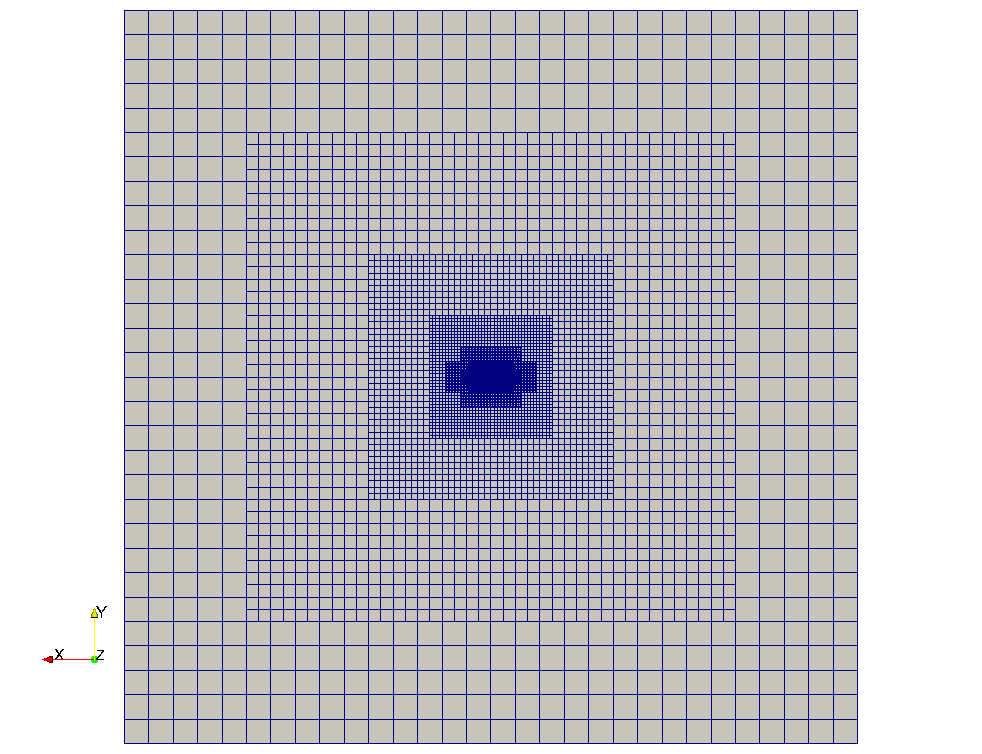
\includegraphics[width=.7\linewidth]{zoomedOutDemo1.png}
  \caption{Zoomed out}
  \label{fig:sub1}
\end{subfigure}%
\\
\begin{subfigure}{\textwidth}
  \centering
  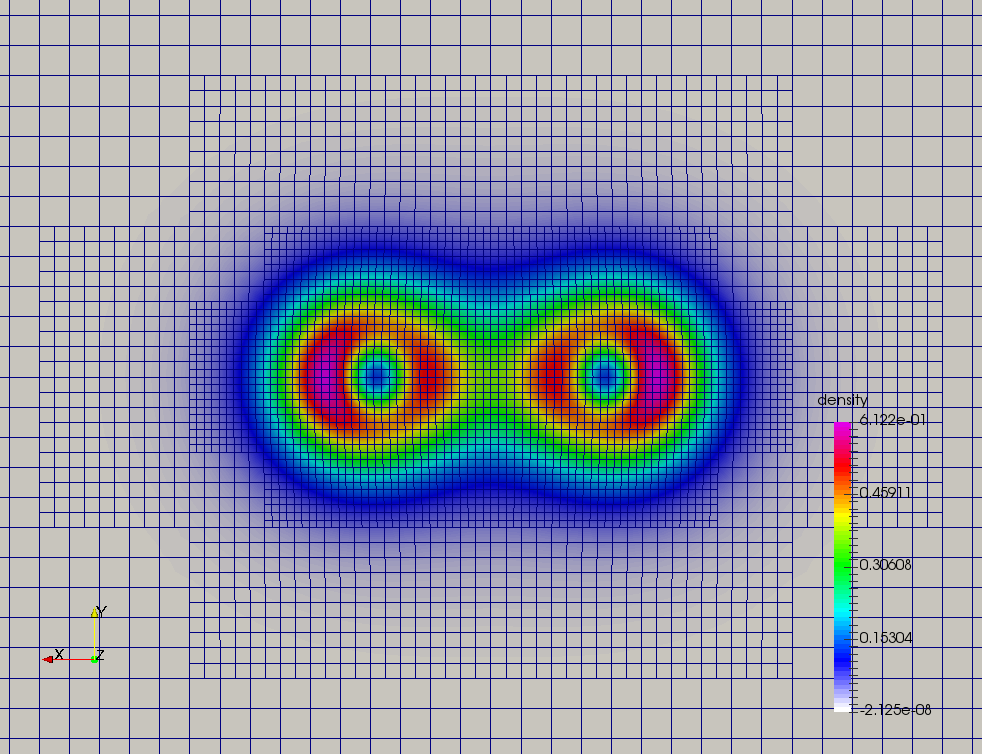
\includegraphics[width=.6\linewidth]{zoomedInDemo1.png}
  \caption{Zoomed in with electron-density contours.}
  \label{fig:sub2}
\end{subfigure}
	\caption{Finite-element mesh used in Nitrogen molecule pseudopotential DFT calculation (See \ref{sec:example1}).}
\label{fig:N2}
\end{figure}

\subsubsection{Example 2}\label{sec:example2}
In the previous example, we discussed how to setup and run a fully non-periodic problem.
Here we briefly discuss how to setup and run the fully periodic problem (FCC Aluminium unit cell) in the folder
\verb|/dftfe/demo/ex2|. There are two input parameter files-- parameterFile\_a.prm and parameterFile\_b.prm. parameterFile\_a.prm is
for computing the ground-state and cell stress of the FCC Al unit cell, while parameterFile\_b.prm additionally does cell stress relaxation.  
Important input parameters in the above parameter files, beyond what we discussed in the previous example are
\begin{enumerate}
\item ``coordinates.inp'' given as input to \verb|ATOMIC COORDINATES FILE|, is the name of an external input file present in the same workspace which lists the fractional (reduced) coordinates of the atoms. For this example, ``coordinates.inp'' is described as 
\begin{verbatim}
13   3   0.00000000E+00   0.00000000E+00   0.00000000E+00
13   3   0.00000000E+00   0.50000000E+00   0.50000000E+00
13   3   0.50000000E+00   0.00000000E+00   0.50000000E+00
13   3   0.50000000E+00   0.50000000E+00   0.00000000E+00
\end{verbatim}
where each line corresponds to ``atomic-charge valence-charge fracx fracy fracz''. {\bf We require fractional coordinates for fully periodic or semi-periodic simulation domains while Cartesian coordinates are mandatory for fully non-periodic simulation domain.}
\item Set fully periodic boundary conditions
\begin{verbatim}	
subsection Boundary conditions
  set PERIODIC1                       = true
  set PERIODIC2                       = true
  set PERIODIC3                       = true
end
\end{verbatim}

\item Inside the \verb|Optimization| subsection, nested within the \verb|Geometry| subsection set 
\begin{verbatim}	
    set CELL STRESS = true
\end{verbatim}	
for computing the ground state cell stress. 

\item 
\begin{verbatim}
subsection Brillouin zone k point sampling options
  set USE TIME REVERSAL SYMMETRY = true
  subsection Monkhorst-Pack (MP) grid generation
    set SAMPLING POINTS 1 = 2
    set SAMPLING POINTS 2 = 2
    set SAMPLING POINTS 3 = 2
    set SAMPLING SHIFT 1  = 1
    set SAMPLING SHIFT 2  = 1
    set SAMPLING SHIFT 3  = 1
  end
end
\end{verbatim}
where
\begin{itemize}
\item \verb|SAMPLING POINTS 1/2/3| sets the number of Monkhorst-Pack grid points to be used along reciprocal lattice
vectors 1, 2, and 3.  		
\item Setting \verb|SAMPLING SHIFT 1/2/3| to 1 enables fractional shifting to be used along reciprocal lattice vectors.
\item Setting \verb|USE TIME REVERSAL SYMMETRY| to true enables use of time reversal symmetry to reduce number of k points to be solved for. For this option to work  \verb|SAMPLING SHIFT 1/2/3| must be set to 1 as done above. 
\end{itemize}

\item Set 
\begin{verbatim}	
subsection Parallelization
  set NPKPT=2
end
\end{verbatim}
which parallelizes the work load of the irreducible k-points across two groups of MPI tasks.

\item The same strategy for convergence of the ground state energy and force discussed
in the previous example is applied to the current example to get convergence in ground state energy and cell stress. 
The ground-state energy per atom and cell stress for finite-element meshes with increasing level of refinement is tabulated in Table~\ref{tab:table2}. Upon comparing the errors in the energy and force with respect the most refined mesh (\emph{Mesh No. 3}), we observe that for \emph{Mesh No. 2} we have obtained convergence in energy per atom to $\mathcal{O}(10^{-5})$ accuracy, and convergence in cell stress to $\mathcal{O}(10^{-6})$ accuracy.
\begin{table}[h!]
  \begin{center}
\small	  
    \caption{FCC Al ground-state energy and cell-stress convergence for demo example 2}
    \label{tab:table2}
    \begin{tabular}{c|c|c|c|c|c} 
	    % <-- Alignments: 1st column left, 2nd middle and 3rd right, with vertical lines in between
	    \hline\hline
	    Mesh No. &\verb|POLYNOMIAL| &\verb|MESH SIZE| & Degrees of freedom& Energy per atom & Cell stress\\
	    &\verb|ORDER| &\verb|AROUND ATOM| & per atom  & (Hartree) & (Hartree/${\rm Bohr}^3$) \\
      \hline
	    1& 4 & 1.0 & 12084 & -2.09082027 &  0.000030750\\	    
	    2& 4 & 0.5 & 27172 & -2.09323142 &  0.000034049\\
	    3&5 & 0.5 & 51239 &  -2.09323871 &  0.000037183\\
       \hline\hline
    \end{tabular}
  \end{center}
\end{table}
The output file using the mesh parameters for \emph{Mesh No.2} is provided at \verb|/demo/ex2/ex2_a.output| (for parameterFile\_a.prm).

\item For cell stress relaxation, use parameterFile\_b.prm, where we set within the \verb|Optimization| subsection nested under \verb|Geometry|
\begin{verbatim}
    set STRESS TOL            = 4e-6
    set CELL OPT              = true
    set CELL CONSTRAINT TYPE  = 1
\end{verbatim}
where
\begin{itemize}
\item \verb|CELL OPT| is set to true which enables cell stress relaxation.  		
\item ``4e-6'' for \verb|STRESS TOL| sets the tolerance of the cell stress (in a.u.) for cell stress relaxation.
\item Choice of ``1'' for \verb|CELL CONSTRAINT TYPE| enforces isotropic shape-fixed volume optimization constraint during cell stress relaxation.
\end{itemize}
For your reference, the output file for the cell stress relaxation is provided at \verb|/demo/ex2/ex2_b.output|. From the output file, you should observe that you obtain a relaxed lattice constant of 7.5719 Bohr after three geometry updates. 
\end{enumerate}



%\section{Future extensions to \dftfe}
%\label{sec:future}
%Some bullet points. To be expanded upon
\begin{itemize}
\item Adaptive meshing
\item Implement improved mixing strategies to decrease the number of SCF iterations.
\item Implement localization strategies to reduce computational cost for for large domain sizes (>1000 atoms).
\item Enriched FEM to reduce computational cost of all-electron calculations.
\item Post-processing tools.
\end{itemize} 


\section{Finding answers to more questions}
\label{sec:questions-and-answers}
If you have questions that go beyond this manual, there are a number of
resources:
\begin{itemize}
\item For questions about \dftfe, installation, bugs, etc., use the 
	\href{https://groups.google.com/forum/#!forum/dftfe-user-group}{DFT-FE discussion forum}. 

\item For latest news, updates, and release announcements about \dftfe{} please send an email to \href{mailto:dft-fe.admin@umich.edu}{dft-fe.admin@umich.edu}, and we will add you to our announcement mailing list.		

\item \dftfe{} is primarily based on the \href{http://www.dealii.org/}{deal.II library}. If you have particular questions
  about deal.II, contact the mailing lists described at \url{https://www.dealii.org/mail.html}.

\item If you have specific questions about \dftfe{} that are not suitable
  for public and archived mailing lists, you can contact the
  primary developers and mentors:
  \begin{itemize}
  \item Phani Motamarri: \url{phanim@umich.edu}.
  \item Sambit Das: \url{dsambit@umich.edu}.
  \item Vikram Gavini: \url{vikramg@umich.edu} (Mentor).
  \end{itemize}
\end{itemize}


\appendix

\section{Run-time input parameters}
\label{sec:parameters}
The underlying description of the input parameters also includes a ``Standard/Advanced/Developer'' label, which signifies whether an input parameter is
a standard one, or an advanced level parameter, or a developer level one only meant for development purposes. The default values of the ``Advanced'' and ``Developer'' labelled parameters are good enough for almost all cases. However, in some cases user may need to use ``Advanced'' labelled parameters. For user convenience,
all input parameters are also indexed at the end of this manual in Section~\ref{sec:runtime-parameter-index-full}.
% now include a file that describes all currently available run-time parameters
\subsection{Global parameters}
\label{parameters:global}


\begin{itemize}

\item {\it Parameter name:} {\tt H REFINED ELECTROSTATICS}
\phantomsection\label{parameters:H REFINED ELECTROSTATICS}
\label{parameters:H_20REFINED_20ELECTROSTATICS}


\index[prmindex]{H REFINED ELECTROSTATICS}
\index[prmindexfull]{H REFINED ELECTROSTATICS}
{\it Value:} false


{\it Default:} false


{\it Description:} [Advanced] Compute electrostatic energy on a h refined mesh after each ground-state solve. Default: false.


{\it Possible values:} A boolean value (true or false)
\item {\it Parameter name:} {\tt KEEP SCRATCH FOLDER}
\phantomsection\label{parameters:KEEP SCRATCH FOLDER}
\label{parameters:KEEP_20SCRATCH_20FOLDER}


\index[prmindex]{KEEP SCRATCH FOLDER}
\index[prmindexfull]{KEEP SCRATCH FOLDER}
{\it Value:} false


{\it Default:} false


{\it Description:} [Advanced] If set to true this option does not delete the dftfeScratch folder when the dftfe object is destroyed. This is useful for debugging and code development. Default: false.


{\it Possible values:} A boolean value (true or false)
\item {\it Parameter name:} {\tt REPRODUCIBLE OUTPUT}
\phantomsection\label{parameters:REPRODUCIBLE OUTPUT}
\label{parameters:REPRODUCIBLE_20OUTPUT}


\index[prmindex]{REPRODUCIBLE OUTPUT}
\index[prmindexfull]{REPRODUCIBLE OUTPUT}
{\it Value:} false


{\it Default:} false


{\it Description:} [Developer] Limit output to what is reproducible, i.e. don't print timing or absolute paths. This parameter is only used for testing purposes.


{\it Possible values:} A boolean value (true or false)
\item {\it Parameter name:} {\tt RESTART}
\phantomsection\label{parameters:RESTART}


\index[prmindex]{RESTART}
\index[prmindexfull]{RESTART}
{\it Value:} false


{\it Default:} false


{\it Description:} [Standard] If set to true RESTART triggers restart checks and modifies the input files for coordinates, domain vectors. Default: false.


{\it Possible values:} A boolean value (true or false)
\item {\it Parameter name:} {\tt RESTART FOLDER}
\phantomsection\label{parameters:RESTART FOLDER}
\label{parameters:RESTART_20FOLDER}


\index[prmindex]{RESTART FOLDER}
\index[prmindexfull]{RESTART FOLDER}
{\it Value:} .


{\it Default:} .


{\it Description:} [Standard] Folder to store restart files.


{\it Possible values:} Any string
\item {\it Parameter name:} {\tt SOLVER MODE}
\phantomsection\label{parameters:SOLVER MODE}
\label{parameters:SOLVER_20MODE}


\index[prmindex]{SOLVER MODE}
\index[prmindexfull]{SOLVER MODE}
{\it Value:} GS


{\it Default:} GS


{\it Description:} [Standard] DFT-FE SOLVER MODE: If GS: performs GroundState calculations, ionic and cell relaxation. If MD: performs Molecular Dynamics Simulation. If NEB: performs a NEB calculation. If GEOOPT: performs an ion and/or cell optimization calculation.


{\it Possible values:} Any one of GS, MD, NEB, GEOOPT
\item {\it Parameter name:} {\tt VERBOSITY}
\phantomsection\label{parameters:VERBOSITY}


\index[prmindex]{VERBOSITY}
\index[prmindexfull]{VERBOSITY}
{\it Value:} 0


{\it Default:} 1


{\it Description:} [Standard] Parameter to control verbosity of terminal output. Ranges from 1 for low, 2 for medium (prints some more additional information), 3 for high (prints eigenvalues and fractional occupancies at the end of each self-consistent field iteration), and 4 for very high, which is only meant for code development purposes. VERBOSITY=0 is only used for unit testing and shouldn't be used by standard users. VERBOSITY=-1 ensures no outout is printed, which is useful when DFT-FE is used as a calculator inside a larger workflow where multiple parallel DFT-FE jobs might be running, for example when using ASE or generating training data for ML workflows.


{\it Possible values:} An integer $n$ such that $-1\leq n \leq 5$
\end{itemize}



\subsection{Parameters in section \tt Boundary conditions}
\label{parameters:Boundary_20conditions}

\begin{itemize}
\item {\it Parameter name:} {\tt CONSTRAINTS FROM SERIAL DOFHANDLER}
\phantomsection\label{parameters:Boundary conditions/CONSTRAINTS FROM SERIAL DOFHANDLER}
\label{parameters:Boundary_20conditions/CONSTRAINTS_20FROM_20SERIAL_20DOFHANDLER}


\index[prmindex]{CONSTRAINTS FROM SERIAL DOFHANDLER}
\index[prmindexfull]{Boundary conditions!CONSTRAINTS FROM SERIAL DOFHANDLER}
{\it Value:} false


{\it Default:} false


{\it Description:} [Developer] Create constraints from serial dofHandler.


{\it Possible values:} A boolean value (true or false)
\item {\it Parameter name:} {\tt CONSTRAINTS PARALLEL CHECK}
\phantomsection\label{parameters:Boundary conditions/CONSTRAINTS PARALLEL CHECK}
\label{parameters:Boundary_20conditions/CONSTRAINTS_20PARALLEL_20CHECK}


\index[prmindex]{CONSTRAINTS PARALLEL CHECK}
\index[prmindexfull]{Boundary conditions!CONSTRAINTS PARALLEL CHECK}
{\it Value:} false


{\it Default:} false


{\it Description:} [Developer] Check for consistency of constraints in parallel.


{\it Possible values:} A boolean value (true or false)
\item {\it Parameter name:} {\tt FLOATING NUCLEAR CHARGES}
\phantomsection\label{parameters:Boundary conditions/FLOATING NUCLEAR CHARGES}
\label{parameters:Boundary_20conditions/FLOATING_20NUCLEAR_20CHARGES}


\index[prmindex]{FLOATING NUCLEAR CHARGES}
\index[prmindexfull]{Boundary conditions!FLOATING NUCLEAR CHARGES}
{\it Value:} true


{\it Default:} true


{\it Description:} [Developer] Nuclear charges are allowed to float independent of the FEM mesh nodal positions. Only allowed for pseudopotential calculations. Internally set to false for all-electron calculations.


{\it Possible values:} A boolean value (true or false)
\item {\it Parameter name:} {\tt PERIODIC1}
\phantomsection\label{parameters:Boundary conditions/PERIODIC1}
\label{parameters:Boundary_20conditions/PERIODIC1}


\index[prmindex]{PERIODIC1}
\index[prmindexfull]{Boundary conditions!PERIODIC1}
{\it Value:} false


{\it Default:} false


{\it Description:} [Standard] Periodicity along the first domain bounding vector.


{\it Possible values:} A boolean value (true or false)
\item {\it Parameter name:} {\tt PERIODIC2}
\phantomsection\label{parameters:Boundary conditions/PERIODIC2}
\label{parameters:Boundary_20conditions/PERIODIC2}


\index[prmindex]{PERIODIC2}
\index[prmindexfull]{Boundary conditions!PERIODIC2}
{\it Value:} false


{\it Default:} false


{\it Description:} [Standard] Periodicity along the second domain bounding vector.


{\it Possible values:} A boolean value (true or false)
\item {\it Parameter name:} {\tt PERIODIC3}
\phantomsection\label{parameters:Boundary conditions/PERIODIC3}
\label{parameters:Boundary_20conditions/PERIODIC3}


\index[prmindex]{PERIODIC3}
\index[prmindexfull]{Boundary conditions!PERIODIC3}
{\it Value:} false


{\it Default:} false


{\it Description:} [Standard] Periodicity along the third domain bounding vector.


{\it Possible values:} A boolean value (true or false)
\item {\it Parameter name:} {\tt POINT WISE DIRICHLET CONSTRAINT}
\phantomsection\label{parameters:Boundary conditions/POINT WISE DIRICHLET CONSTRAINT}
\label{parameters:Boundary_20conditions/POINT_20WISE_20DIRICHLET_20CONSTRAINT}


\index[prmindex]{POINT WISE DIRICHLET CONSTRAINT}
\index[prmindexfull]{Boundary conditions!POINT WISE DIRICHLET CONSTRAINT}
{\it Value:} false


{\it Default:} false


{\it Description:} [Developer] Flag to set point wise dirichlet constraints to eliminate null-space associated with the discretized Poisson operator subject to periodic BCs.


{\it Possible values:} A boolean value (true or false)
\item {\it Parameter name:} {\tt SELF POTENTIAL RADIUS}
\phantomsection\label{parameters:Boundary conditions/SELF POTENTIAL RADIUS}
\label{parameters:Boundary_20conditions/SELF_20POTENTIAL_20RADIUS}


\index[prmindex]{SELF POTENTIAL RADIUS}
\index[prmindexfull]{Boundary conditions!SELF POTENTIAL RADIUS}
{\it Value:} 0.0


{\it Default:} 0.0


{\it Description:} [Advanced] The radius (in a.u) of the ball around an atom in which self-potential of the associated nuclear charge is solved. For the default value of 0.0, the radius value is automatically determined to accommodate the largest radius possible for the given finite element mesh. The default approach works for most problems.


{\it Possible values:} A floating point number $v$ such that $0 \leq v \leq 50$
\item {\it Parameter name:} {\tt SMEARED NUCLEAR CHARGES}
\phantomsection\label{parameters:Boundary conditions/SMEARED NUCLEAR CHARGES}
\label{parameters:Boundary_20conditions/SMEARED_20NUCLEAR_20CHARGES}


\index[prmindex]{SMEARED NUCLEAR CHARGES}
\index[prmindexfull]{Boundary conditions!SMEARED NUCLEAR CHARGES}
{\it Value:} true


{\it Default:} true


{\it Description:} [Developer] Nuclear charges are smeared for solving electrostatic fields. Default is true for pseudopotential calculations and false for all-electron calculations.


{\it Possible values:} A boolean value (true or false)
\end{itemize}

\subsection{Parameters in section \tt Brillouin zone k point sampling options}
\label{parameters:Brillouin_20zone_20k_20point_20sampling_20options}

\begin{itemize}
\item {\it Parameter name:} {\tt USE GROUP SYMMETRY}
\phantomsection\label{parameters:Brillouin zone k point sampling options/USE GROUP SYMMETRY}
\label{parameters:Brillouin_20zone_20k_20point_20sampling_20options/USE_20GROUP_20SYMMETRY}


\index[prmindex]{USE GROUP SYMMETRY}
\index[prmindexfull]{Brillouin zone k point sampling options!USE GROUP SYMMETRY}
{\it Value:} false


{\it Default:} false


{\it Description:} [Standard] Flag to control the use of point group symmetries. Currently this feature cannot be used if ION FORCE or CELL STRESS input parameters are set to true.


{\it Possible values:} A boolean value (true or false)
\item {\it Parameter name:} {\tt USE TIME REVERSAL SYMMETRY}
\phantomsection\label{parameters:Brillouin zone k point sampling options/USE TIME REVERSAL SYMMETRY}
\label{parameters:Brillouin_20zone_20k_20point_20sampling_20options/USE_20TIME_20REVERSAL_20SYMMETRY}


\index[prmindex]{USE TIME REVERSAL SYMMETRY}
\index[prmindexfull]{Brillouin zone k point sampling options!USE TIME REVERSAL SYMMETRY}
{\it Value:} false


{\it Default:} false


{\it Description:} [Standard] Flag to control the use of time reversal symmetry.


{\it Possible values:} A boolean value (true or false)
\item {\it Parameter name:} {\tt kPOINT RULE FILE}
\phantomsection\label{parameters:Brillouin zone k point sampling options/kPOINT RULE FILE}
\label{parameters:Brillouin_20zone_20k_20point_20sampling_20options/kPOINT_20RULE_20FILE}


\index[prmindex]{kPOINT RULE FILE}
\index[prmindexfull]{Brillouin zone k point sampling options!kPOINT RULE FILE}
{\it Value:} 


{\it Default:} 


{\it Description:} [Developer] File providing list of k points on which eigen values are to be computed from converged KS Hamiltonian. The first three columns specify the crystal coordinates of the k points. The fourth column provides weights of the corresponding points, which is currently not used. The eigen values are written on an output file bands.out


{\it Possible values:} Any string
\end{itemize}



\subsection{Parameters in section \tt Brillouin zone k point sampling options/Monkhorst-Pack (MP) grid generation}
\label{parameters:Brillouin_20zone_20k_20point_20sampling_20options/Monkhorst_2dPack_20_28MP_29_20grid_20generation}

\begin{itemize}
\item {\it Parameter name:} {\tt SAMPLING POINTS 1}
\phantomsection\label{parameters:Brillouin zone k point sampling options/Monkhorst_2dPack _28MP_29 grid generation/SAMPLING POINTS 1}
\label{parameters:Brillouin_20zone_20k_20point_20sampling_20options/Monkhorst_2dPack_20_28MP_29_20grid_20generation/SAMPLING_20POINTS_201}


\index[prmindex]{SAMPLING POINTS 1}
\index[prmindexfull]{Brillouin zone k point sampling options!Monkhorst-Pack (MP) grid generation!SAMPLING POINTS 1}
{\it Value:} 1


{\it Default:} 1


{\it Description:} [Standard] Number of Monkhorst-Pack grid points to be used along reciprocal lattice vector 1.


{\it Possible values:} An integer $n$ such that $1\leq n \leq 1000$
\item {\it Parameter name:} {\tt SAMPLING POINTS 2}
\phantomsection\label{parameters:Brillouin zone k point sampling options/Monkhorst_2dPack _28MP_29 grid generation/SAMPLING POINTS 2}
\label{parameters:Brillouin_20zone_20k_20point_20sampling_20options/Monkhorst_2dPack_20_28MP_29_20grid_20generation/SAMPLING_20POINTS_202}


\index[prmindex]{SAMPLING POINTS 2}
\index[prmindexfull]{Brillouin zone k point sampling options!Monkhorst-Pack (MP) grid generation!SAMPLING POINTS 2}
{\it Value:} 1


{\it Default:} 1


{\it Description:} [Standard] Number of Monkhorst-Pack grid points to be used along reciprocal lattice vector 2.


{\it Possible values:} An integer $n$ such that $1\leq n \leq 1000$
\item {\it Parameter name:} {\tt SAMPLING POINTS 3}
\phantomsection\label{parameters:Brillouin zone k point sampling options/Monkhorst_2dPack _28MP_29 grid generation/SAMPLING POINTS 3}
\label{parameters:Brillouin_20zone_20k_20point_20sampling_20options/Monkhorst_2dPack_20_28MP_29_20grid_20generation/SAMPLING_20POINTS_203}


\index[prmindex]{SAMPLING POINTS 3}
\index[prmindexfull]{Brillouin zone k point sampling options!Monkhorst-Pack (MP) grid generation!SAMPLING POINTS 3}
{\it Value:} 1


{\it Default:} 1


{\it Description:} [Standard] Number of Monkhorst-Pack grid points to be used along reciprocal lattice vector 3.


{\it Possible values:} An integer $n$ such that $1\leq n \leq 1000$
\item {\it Parameter name:} {\tt SAMPLING SHIFT 1}
\phantomsection\label{parameters:Brillouin zone k point sampling options/Monkhorst_2dPack _28MP_29 grid generation/SAMPLING SHIFT 1}
\label{parameters:Brillouin_20zone_20k_20point_20sampling_20options/Monkhorst_2dPack_20_28MP_29_20grid_20generation/SAMPLING_20SHIFT_201}


\index[prmindex]{SAMPLING SHIFT 1}
\index[prmindexfull]{Brillouin zone k point sampling options!Monkhorst-Pack (MP) grid generation!SAMPLING SHIFT 1}
{\it Value:} 0


{\it Default:} 0


{\it Description:} [Standard] If fractional shifting to be used (0 for no shift, 1 for shift) along reciprocal lattice vector 1.


{\it Possible values:} An integer $n$ such that $0\leq n \leq 1$
\item {\it Parameter name:} {\tt SAMPLING SHIFT 2}
\phantomsection\label{parameters:Brillouin zone k point sampling options/Monkhorst_2dPack _28MP_29 grid generation/SAMPLING SHIFT 2}
\label{parameters:Brillouin_20zone_20k_20point_20sampling_20options/Monkhorst_2dPack_20_28MP_29_20grid_20generation/SAMPLING_20SHIFT_202}


\index[prmindex]{SAMPLING SHIFT 2}
\index[prmindexfull]{Brillouin zone k point sampling options!Monkhorst-Pack (MP) grid generation!SAMPLING SHIFT 2}
{\it Value:} 0


{\it Default:} 0


{\it Description:} [Standard] If fractional shifting to be used (0 for no shift, 1 for shift) along reciprocal lattice vector 2.


{\it Possible values:} An integer $n$ such that $0\leq n \leq 1$
\item {\it Parameter name:} {\tt SAMPLING SHIFT 3}
\phantomsection\label{parameters:Brillouin zone k point sampling options/Monkhorst_2dPack _28MP_29 grid generation/SAMPLING SHIFT 3}
\label{parameters:Brillouin_20zone_20k_20point_20sampling_20options/Monkhorst_2dPack_20_28MP_29_20grid_20generation/SAMPLING_20SHIFT_203}


\index[prmindex]{SAMPLING SHIFT 3}
\index[prmindexfull]{Brillouin zone k point sampling options!Monkhorst-Pack (MP) grid generation!SAMPLING SHIFT 3}
{\it Value:} 0


{\it Default:} 0


{\it Description:} [Standard] If fractional shifting to be used (0 for no shift, 1 for shift) along reciprocal lattice vector 3.


{\it Possible values:} An integer $n$ such that $0\leq n \leq 1$
\end{itemize}

\subsection{Parameters in section \tt Checkpointing and Restart}
\label{parameters:Checkpointing_20and_20Restart}

\begin{itemize}
\item {\it Parameter name:} {\tt CHK TYPE}
\phantomsection\label{parameters:Checkpointing and Restart/CHK TYPE}
\label{parameters:Checkpointing_20and_20Restart/CHK_20TYPE}


\index[prmindex]{CHK TYPE}
\index[prmindexfull]{Checkpointing and Restart!CHK TYPE}
{\it Value:} 0


{\it Default:} 0


{\it Description:} [Standard] Checkpoint type, 0 (do not create any checkpoint), 1 (create checkpoint for geometry optimization restart if either ION OPT or CELL OPT is set to true. Currently, checkpointing and restart framework does not work if both ION OPT and CELL OPT are set to true simultaneously- the code will throw an error if attempted.), 2 (create checkpoint for scf restart using the electron-density field. Currently, this option cannot be used if geometry optimization is being performed. The code will throw an error if this option is used in conjunction with geometry optimization.)


{\it Possible values:} An integer $n$ such that $0\leq n \leq 2$
\item {\it Parameter name:} {\tt RESTART FROM CHK}
\phantomsection\label{parameters:Checkpointing and Restart/RESTART FROM CHK}
\label{parameters:Checkpointing_20and_20Restart/RESTART_20FROM_20CHK}


\index[prmindex]{RESTART FROM CHK}
\index[prmindexfull]{Checkpointing and Restart!RESTART FROM CHK}
{\it Value:} false


{\it Default:} false


{\it Description:} [Standard] Boolean parameter specifying if the current job reads from a checkpoint. The nature of the restart corresponds to the CHK TYPE parameter. Hence, the checkpoint being read must have been created using the CHK TYPE parameter before using this option. Further, for CHK TYPE=2 same number of MPI tasks must be used as used to create the checkpoint files. RESTART FROM CHK is always false for CHK TYPE 0.


{\it Possible values:} A boolean value (true or false)
\item {\it Parameter name:} {\tt RESTART SP FROM NO SP}
\phantomsection\label{parameters:Checkpointing and Restart/RESTART SP FROM NO SP}
\label{parameters:Checkpointing_20and_20Restart/RESTART_20SP_20FROM_20NO_20SP}


\index[prmindex]{RESTART SP FROM NO SP}
\index[prmindexfull]{Checkpointing and Restart!RESTART SP FROM NO SP}
{\it Value:} false


{\it Default:} false


{\it Description:} [Standard] Enables ground-state solve for SPIN POLARIZED case reading the SPIN UNPOLARIZED density from the checkpoint files, and use the START MAGNETIZATION to compute the spin up and spin down densities. This option is only valid for CHK TYPE=2 and RESTART FROM CHK=true. Default false..


{\it Possible values:} A boolean value (true or false)
\end{itemize}

\subsection{Parameters in section \tt DFT functional parameters}
\label{parameters:DFT_20functional_20parameters}

\begin{itemize}
\item {\it Parameter name:} {\tt EXCHANGE CORRELATION TYPE}
\phantomsection\label{parameters:DFT functional parameters/EXCHANGE CORRELATION TYPE}
\label{parameters:DFT_20functional_20parameters/EXCHANGE_20CORRELATION_20TYPE}


\index[prmindex]{EXCHANGE CORRELATION TYPE}
\index[prmindexfull]{DFT functional parameters!EXCHANGE CORRELATION TYPE}
{\it Value:} 4


{\it Default:} 1


{\it Description:} [Standard] Parameter specifying the type of exchange-correlation to be used: 1(LDA: Perdew Zunger Ceperley Alder correlation with Slater Exchange[PRB. 23, 5048 (1981)]), 2(LDA: Perdew-Wang 92 functional with Slater Exchange [PRB. 45, 13244 (1992)]), 3(LDA: Vosko, Wilk \& Nusair with Slater Exchange[Can. J. Phys. 58, 1200 (1980)]), 4(GGA: Perdew-Burke-Ernzerhof functional [PRL. 77, 3865 (1996)], 5(RPBE: B. Hammer, L. B. Hansen, and J. K. Nørskov, Phys. Rev. B 59, 7413 (1999)).


{\it Possible values:} An integer $n$ such that $1\leq n \leq 5$
\item {\it Parameter name:} {\tt NUMBER OF IMAGES}
\phantomsection\label{parameters:DFT functional parameters/NUMBER OF IMAGES}
\label{parameters:DFT_20functional_20parameters/NUMBER_20OF_20IMAGES}


\index[prmindex]{NUMBER OF IMAGES}
\index[prmindexfull]{DFT functional parameters!NUMBER OF IMAGES}
{\it Value:} 1


{\it Default:} 1


{\it Description:} [Standard] NUMBER OF IMAGES:Default option is 1. When NEB is triggered this controls the total number of images along the MEP including the end points


{\it Possible values:} An integer $n$ such that $1\leq n \leq 50$
\item {\it Parameter name:} {\tt PSEUDOPOTENTIAL CALCULATION}
\phantomsection\label{parameters:DFT functional parameters/PSEUDOPOTENTIAL CALCULATION}
\label{parameters:DFT_20functional_20parameters/PSEUDOPOTENTIAL_20CALCULATION}


\index[prmindex]{PSEUDOPOTENTIAL CALCULATION}
\index[prmindexfull]{DFT functional parameters!PSEUDOPOTENTIAL CALCULATION}
{\it Value:} true


{\it Default:} true


{\it Description:} [Standard] Boolean Parameter specifying whether pseudopotential DFT calculation needs to be performed. For all-electron DFT calculation set to false.


{\it Possible values:} A boolean value (true or false)
\item {\it Parameter name:} {\tt PSEUDOPOTENTIAL FILE NAMES LIST}
\phantomsection\label{parameters:DFT functional parameters/PSEUDOPOTENTIAL FILE NAMES LIST}
\label{parameters:DFT_20functional_20parameters/PSEUDOPOTENTIAL_20FILE_20NAMES_20LIST}


\index[prmindex]{PSEUDOPOTENTIAL FILE NAMES LIST}
\index[prmindexfull]{DFT functional parameters!PSEUDOPOTENTIAL FILE NAMES LIST}
{\it Value:} pseudo.inp


{\it Default:} 


{\it Description:} [Standard] Pseudopotential file. This file contains the list of pseudopotential file names in UPF format corresponding to the atoms involved in the calculations. UPF version 2.0 or greater and norm-conserving pseudopotentials(ONCV and Troullier Martins) in UPF format are only accepted. File format (example for two atoms Mg(z=12), Al(z=13)): 12 filename1.upf(row1), 13 filename2.upf (row2). Important Note: ONCV pseudopotentials data base in UPF format can be downloaded from http://www.quantum-simulation.org/potentials/sg15\_oncv or http://www.pseudo-dojo.org/.  Troullier-Martins pseudopotentials in UPF format can be downloaded from http://www.quantum-espresso.org/pseudopotentials/fhi-pp-from-abinit-web-site.


{\it Possible values:} Any string
\item {\it Parameter name:} {\tt PSEUDO TESTS FLAG}
\phantomsection\label{parameters:DFT functional parameters/PSEUDO TESTS FLAG}
\label{parameters:DFT_20functional_20parameters/PSEUDO_20TESTS_20FLAG}


\index[prmindex]{PSEUDO TESTS FLAG}
\index[prmindexfull]{DFT functional parameters!PSEUDO TESTS FLAG}
{\it Value:} false


{\it Default:} false


{\it Description:} [Developer] Boolean parameter specifying the explicit path of pseudopotential upf format files used for ctests


{\it Possible values:} A boolean value (true or false)
\item {\it Parameter name:} {\tt PSP CUTOFF IMAGE CHARGES}
\phantomsection\label{parameters:DFT functional parameters/PSP CUTOFF IMAGE CHARGES}
\label{parameters:DFT_20functional_20parameters/PSP_20CUTOFF_20IMAGE_20CHARGES}


\index[prmindex]{PSP CUTOFF IMAGE CHARGES}
\index[prmindexfull]{DFT functional parameters!PSP CUTOFF IMAGE CHARGES}
{\it Value:} 15.0


{\it Default:} 15.0


{\it Description:} [Standard] Distance from the domain till which periodic images will be considered for the local part of the pseudopotential. Units in a.u. 


{\it Possible values:} A floating point number $v$ such that $-\text{MAX\_DOUBLE} \leq v \leq \text{MAX\_DOUBLE}$
\item {\it Parameter name:} {\tt SPIN POLARIZATION}
\phantomsection\label{parameters:DFT functional parameters/SPIN POLARIZATION}
\label{parameters:DFT_20functional_20parameters/SPIN_20POLARIZATION}


\index[prmindex]{SPIN POLARIZATION}
\index[prmindexfull]{DFT functional parameters!SPIN POLARIZATION}
{\it Value:} 0


{\it Default:} 0


{\it Description:} [Standard] Spin polarization: 0 for no spin polarization and 1 for collinear spin polarization calculation. Default option is 0.


{\it Possible values:} An integer $n$ such that $0\leq n \leq 1$
\item {\it Parameter name:} {\tt START MAGNETIZATION}
\phantomsection\label{parameters:DFT functional parameters/START MAGNETIZATION}
\label{parameters:DFT_20functional_20parameters/START_20MAGNETIZATION}


\index[prmindex]{START MAGNETIZATION}
\index[prmindexfull]{DFT functional parameters!START MAGNETIZATION}
{\it Value:} 0.0


{\it Default:} 0.0


{\it Description:} [Standard] Starting magnetization to be used for spin-polarized DFT calculations (must be between -0.5 and +0.5). Corresponding magnetization per simulation domain will be (2 x START MAGNETIZATION x Number of electrons) a.u. 


{\it Possible values:} A floating point number $v$ such that $-0.5 \leq v \leq 0.5$
\end{itemize}



\subsection{Parameters in section \tt DFT functional parameters/Dispersion Correction}
\label{parameters:DFT_20functional_20parameters/Dispersion_20Correction}

\begin{itemize}
\item {\it Parameter name:} {\tt CN CUTOFF}
\phantomsection\label{parameters:DFT functional parameters/Dispersion Correction/CN CUTOFF}
\label{parameters:DFT_20functional_20parameters/Dispersion_20Correction/CN_20CUTOFF}


\index[prmindex]{CN CUTOFF}
\index[prmindexfull]{DFT functional parameters!Dispersion Correction!CN CUTOFF}
{\it Value:} 40.0


{\it Default:} 40.0


{\it Description:} [Advanced] Cutoff in a.u. for computing coordination number in D3 correction


{\it Possible values:} A floating point number $v$ such that $0 \leq v \leq \text{MAX\_DOUBLE}$
\item {\it Parameter name:} {\tt D3 ATM}
\phantomsection\label{parameters:DFT functional parameters/Dispersion Correction/D3 ATM}
\label{parameters:DFT_20functional_20parameters/Dispersion_20Correction/D3_20ATM}


\index[prmindex]{D3 ATM}
\index[prmindexfull]{DFT functional parameters!Dispersion Correction!D3 ATM}
{\it Value:} false


{\it Default:} false


{\it Description:} [Standard] Boolean parameter specifying whether or not the triple dipole correction in DFTD3 is to be included (ignored if DAMPING PARAMETERS FILE is specified).


{\it Possible values:} A boolean value (true or false)
\item {\it Parameter name:} {\tt D3 DAMPING TYPE}
\phantomsection\label{parameters:DFT functional parameters/Dispersion Correction/D3 DAMPING TYPE}
\label{parameters:DFT_20functional_20parameters/Dispersion_20Correction/D3_20DAMPING_20TYPE}


\index[prmindex]{D3 DAMPING TYPE}
\index[prmindexfull]{DFT functional parameters!Dispersion Correction!D3 DAMPING TYPE}
{\it Value:} 3


{\it Default:} 3


{\it Description:} [Standard] The damping used for DFTD3, 0 for zero damping, 1 for BJ damping, 2 for D3M variant, 3 for BJM variant (default) and 4 for the OP variant.


{\it Possible values:} An integer $n$ such that $0\leq n \leq 4$
\item {\it Parameter name:} {\tt D4 MBD}
\phantomsection\label{parameters:DFT functional parameters/Dispersion Correction/D4 MBD}
\label{parameters:DFT_20functional_20parameters/Dispersion_20Correction/D4_20MBD}


\index[prmindex]{D4 MBD}
\index[prmindexfull]{DFT functional parameters!Dispersion Correction!D4 MBD}
{\it Value:} false


{\it Default:} false


{\it Description:} [Standard] Boolean parameter specifying whether or not the MBD correction in DFTD4 is to be included (ignored if DAMPING PARAMETERS FILE is specified).


{\it Possible values:} A boolean value (true or false)
\item {\it Parameter name:} {\tt DAMPING PARAMETERS FILE}
\phantomsection\label{parameters:DFT functional parameters/Dispersion Correction/DAMPING PARAMETERS FILE}
\label{parameters:DFT_20functional_20parameters/Dispersion_20Correction/DAMPING_20PARAMETERS_20FILE}


\index[prmindex]{DAMPING PARAMETERS FILE}
\index[prmindexfull]{DFT functional parameters!Dispersion Correction!DAMPING PARAMETERS FILE}
{\it Value:} 


{\it Default:} 


{\it Description:} [Advanced] Name of the file containing custom damping parameters, for ZERO damping 6 parameters are expected (s6, s8, s9, sr6, sr8, alpha), for BJ anf BJM damping 6 parameters are expected (s6, s8, s9, a1, a2, alpha), for ZEROM damping 7 parameters are expected (s6, s8, s9, sr6, sr8, alpha, beta) and for optimized power damping 7 parameters are expected (s6, s8, s9, a1, a2, alpha, beta).


{\it Possible values:} Any string
\item {\it Parameter name:} {\tt DISPERSION CORRECTION TYPE}
\phantomsection\label{parameters:DFT functional parameters/Dispersion Correction/DISPERSION CORRECTION TYPE}
\label{parameters:DFT_20functional_20parameters/Dispersion_20Correction/DISPERSION_20CORRECTION_20TYPE}


\index[prmindex]{DISPERSION CORRECTION TYPE}
\index[prmindexfull]{DFT functional parameters!Dispersion Correction!DISPERSION CORRECTION TYPE}
{\it Value:} 0


{\it Default:} 0


{\it Description:} [Standard] The dispersion correction type to be included post scf convergence: 0 for none, 1 for DFT-D3[JCP 132, 154104 (2010)][JCC 32, 1456 (2011)], 2 for DFT-D4 [JCP 147, 034112 (2017)][JCP 150, 154122 (2019)][PCCP 22, 8499-8512 (2020)].


{\it Possible values:} An integer $n$ such that $0\leq n \leq 2$
\item {\it Parameter name:} {\tt THREE BODY CUTOFF}
\phantomsection\label{parameters:DFT functional parameters/Dispersion Correction/THREE BODY CUTOFF}
\label{parameters:DFT_20functional_20parameters/Dispersion_20Correction/THREE_20BODY_20CUTOFF}


\index[prmindex]{THREE BODY CUTOFF}
\index[prmindexfull]{DFT functional parameters!Dispersion Correction!THREE BODY CUTOFF}
{\it Value:} 40.0


{\it Default:} 40.0


{\it Description:} [Advanced] Cutoff in a.u. for computing 3 body interactions terms in D3 correction


{\it Possible values:} A floating point number $v$ such that $0 \leq v \leq \text{MAX\_DOUBLE}$
\item {\it Parameter name:} {\tt TWO BODY CUTOFF}
\phantomsection\label{parameters:DFT functional parameters/Dispersion Correction/TWO BODY CUTOFF}
\label{parameters:DFT_20functional_20parameters/Dispersion_20Correction/TWO_20BODY_20CUTOFF}


\index[prmindex]{TWO BODY CUTOFF}
\index[prmindexfull]{DFT functional parameters!Dispersion Correction!TWO BODY CUTOFF}
{\it Value:} 94.8683298050514


{\it Default:} 94.8683298050514


{\it Description:} [Advanced] Cutoff in a.u. for computing 2 body interactions terms in D3 correction


{\it Possible values:} A floating point number $v$ such that $0 \leq v \leq \text{MAX\_DOUBLE}$
\end{itemize}

\subsection{Parameters in section \tt Finite element mesh parameters}
\label{parameters:Finite_20element_20mesh_20parameters}

\begin{itemize}
\item {\it Parameter name:} {\tt POLYNOMIAL ORDER}
\phantomsection\label{parameters:Finite element mesh parameters/POLYNOMIAL ORDER}
\label{parameters:Finite_20element_20mesh_20parameters/POLYNOMIAL_20ORDER}


\index[prmindex]{POLYNOMIAL ORDER}
\index[prmindexfull]{Finite element mesh parameters!POLYNOMIAL ORDER}
{\it Value:} 6


{\it Default:} 6


{\it Description:} [Standard] The degree of the finite-element interpolating polynomial in the Kohn-Sham Hamitonian except the electrostatics. Default value is 6 which is good choice for most pseudopotential calculations. POLYNOMIAL ORDER= 4 or 5 is usually a good choice for all-electron problems.


{\it Possible values:} An integer $n$ such that $1\leq n \leq 12$
\item {\it Parameter name:} {\tt POLYNOMIAL ORDER ELECTROSTATICS}
\phantomsection\label{parameters:Finite element mesh parameters/POLYNOMIAL ORDER ELECTROSTATICS}
\label{parameters:Finite_20element_20mesh_20parameters/POLYNOMIAL_20ORDER_20ELECTROSTATICS}


\index[prmindex]{POLYNOMIAL ORDER ELECTROSTATICS}
\index[prmindexfull]{Finite element mesh parameters!POLYNOMIAL ORDER ELECTROSTATICS}
{\it Value:} 0


{\it Default:} 0


{\it Description:} [Standard] The degree of the finite-element interpolating polynomial for the electrostatics part of the Kohn-Sham Hamiltonian. It is automatically set to POLYNOMIAL ORDER if POLYNOMIAL ORDER ELECTROSTATICS set to default value of zero.


{\it Possible values:} An integer $n$ such that $0\leq n \leq 24$
\end{itemize}



\subsection{Parameters in section \tt Finite element mesh parameters/Auto mesh generation parameters}
\label{parameters:Finite_20element_20mesh_20parameters/Auto_20mesh_20generation_20parameters}

\begin{itemize}
\item {\it Parameter name:} {\tt ATOM BALL RADIUS}
\phantomsection\label{parameters:Finite element mesh parameters/Auto mesh generation parameters/ATOM BALL RADIUS}
\label{parameters:Finite_20element_20mesh_20parameters/Auto_20mesh_20generation_20parameters/ATOM_20BALL_20RADIUS}


\index[prmindex]{ATOM BALL RADIUS}
\index[prmindexfull]{Finite element mesh parameters!Auto mesh generation parameters!ATOM BALL RADIUS}
{\it Value:} 3


{\it Default:} 0.0


{\it Description:} [Standard] Radius of ball enclosing every atom, inside which the mesh size is set close to MESH SIZE AROUND ATOM and coarse-grained in the region outside the enclosing balls. For the default value of 0.0, a heuristically determined value is used, which is good enough for most cases but can be a bit conservative choice for fully non-periodic and semi-periodic problems as well as all-electron problems. To improve the computational efficiency user may experiment with values of ATOM BALL RADIUS ranging between 3.0 to 6.0 for pseudopotential problems, and ranging between 1.0 to 2.5 for all-electron problems.  Units: a.u.


{\it Possible values:} A floating point number $v$ such that $0 \leq v \leq 20$
\item {\it Parameter name:} {\tt AUTO ADAPT BASE MESH SIZE}
\phantomsection\label{parameters:Finite element mesh parameters/Auto mesh generation parameters/AUTO ADAPT BASE MESH SIZE}
\label{parameters:Finite_20element_20mesh_20parameters/Auto_20mesh_20generation_20parameters/AUTO_20ADAPT_20BASE_20MESH_20SIZE}


\index[prmindex]{AUTO ADAPT BASE MESH SIZE}
\index[prmindexfull]{Finite element mesh parameters!Auto mesh generation parameters!AUTO ADAPT BASE MESH SIZE}
{\it Value:} true


{\it Default:} true


{\it Description:} [Developer] Automatically adapt the BASE MESH SIZE such that subdivisions of that during refinement leads closest to the desired MESH SIZE AROUND ATOM. Default: true.


{\it Possible values:} A boolean value (true or false)
\item {\it Parameter name:} {\tt BASE MESH SIZE}
\phantomsection\label{parameters:Finite element mesh parameters/Auto mesh generation parameters/BASE MESH SIZE}
\label{parameters:Finite_20element_20mesh_20parameters/Auto_20mesh_20generation_20parameters/BASE_20MESH_20SIZE}


\index[prmindex]{BASE MESH SIZE}
\index[prmindexfull]{Finite element mesh parameters!Auto mesh generation parameters!BASE MESH SIZE}
{\it Value:} 0.0


{\it Default:} 0.0


{\it Description:} [Advanced] Mesh size of the base mesh on which refinement is performed. For the default value of 0.0, a heuristically determined base mesh size is used, which is good enough for most cases. Standard users do not need to tune this parameter. Units: a.u.


{\it Possible values:} A floating point number $v$ such that $0 \leq v \leq 20$
\item {\it Parameter name:} {\tt ERROR ESTIMATE WAVEFUNCTIONS}
\phantomsection\label{parameters:Finite element mesh parameters/Auto mesh generation parameters/ERROR ESTIMATE WAVEFUNCTIONS}
\label{parameters:Finite_20element_20mesh_20parameters/Auto_20mesh_20generation_20parameters/ERROR_20ESTIMATE_20WAVEFUNCTIONS}


\index[prmindex]{ERROR ESTIMATE WAVEFUNCTIONS}
\index[prmindexfull]{Finite element mesh parameters!Auto mesh generation parameters!ERROR ESTIMATE WAVEFUNCTIONS}
{\it Value:} 5


{\it Default:} 5


{\it Description:} [Developer] Number of wavefunctions to be used for error estimation.


{\it Possible values:} An integer $n$ such that $0\leq n \leq 2147483647$
\item {\it Parameter name:} {\tt GAUSSIAN CONSTANT FORCE GENERATOR}
\phantomsection\label{parameters:Finite element mesh parameters/Auto mesh generation parameters/GAUSSIAN CONSTANT FORCE GENERATOR}
\label{parameters:Finite_20element_20mesh_20parameters/Auto_20mesh_20generation_20parameters/GAUSSIAN_20CONSTANT_20FORCE_20GENERATOR}


\index[prmindex]{GAUSSIAN CONSTANT FORCE GENERATOR}
\index[prmindexfull]{Finite element mesh parameters!Auto mesh generation parameters!GAUSSIAN CONSTANT FORCE GENERATOR}
{\it Value:} 0.75


{\it Default:} 0.75


{\it Description:} [Developer] Force computation generator gaussian constant. Also used for mesh movement. Gamma(r)= exp(-(r/gaussianConstant);(gaussianOrder)).


{\it Possible values:} A floating point number $v$ such that $0 \leq v \leq \text{MAX\_DOUBLE}$
\item {\it Parameter name:} {\tt GAUSSIAN ORDER FORCE GENERATOR}
\phantomsection\label{parameters:Finite element mesh parameters/Auto mesh generation parameters/GAUSSIAN ORDER FORCE GENERATOR}
\label{parameters:Finite_20element_20mesh_20parameters/Auto_20mesh_20generation_20parameters/GAUSSIAN_20ORDER_20FORCE_20GENERATOR}


\index[prmindex]{GAUSSIAN ORDER FORCE GENERATOR}
\index[prmindexfull]{Finite element mesh parameters!Auto mesh generation parameters!GAUSSIAN ORDER FORCE GENERATOR}
{\it Value:} 4.0


{\it Default:} 4.0


{\it Description:} [Developer] Force computation generator gaussian order. Also used for mesh movement. Gamma(r)= exp(-(r/gaussianConstant);(gaussianOrder)).


{\it Possible values:} A floating point number $v$ such that $0 \leq v \leq \text{MAX\_DOUBLE}$
\item {\it Parameter name:} {\tt GAUSSIAN ORDER MOVE MESH TO ATOMS}
\phantomsection\label{parameters:Finite element mesh parameters/Auto mesh generation parameters/GAUSSIAN ORDER MOVE MESH TO ATOMS}
\label{parameters:Finite_20element_20mesh_20parameters/Auto_20mesh_20generation_20parameters/GAUSSIAN_20ORDER_20MOVE_20MESH_20TO_20ATOMS}


\index[prmindex]{GAUSSIAN ORDER MOVE MESH TO ATOMS}
\index[prmindexfull]{Finite element mesh parameters!Auto mesh generation parameters!GAUSSIAN ORDER MOVE MESH TO ATOMS}
{\it Value:} 4.0


{\it Default:} 4.0


{\it Description:} [Developer] Move mesh to atoms gaussian order. Gamma(r)= exp(-(r/gaussianConstant);(gaussianOrder)).


{\it Possible values:} A floating point number $v$ such that $0 \leq v \leq \text{MAX\_DOUBLE}$
\item {\it Parameter name:} {\tt INNER ATOM BALL RADIUS}
\phantomsection\label{parameters:Finite element mesh parameters/Auto mesh generation parameters/INNER ATOM BALL RADIUS}
\label{parameters:Finite_20element_20mesh_20parameters/Auto_20mesh_20generation_20parameters/INNER_20ATOM_20BALL_20RADIUS}


\index[prmindex]{INNER ATOM BALL RADIUS}
\index[prmindexfull]{Finite element mesh parameters!Auto mesh generation parameters!INNER ATOM BALL RADIUS}
{\it Value:} 0.0


{\it Default:} 0.0


{\it Description:} [Advanced] Radius of ball enclosing every atom, inside which the mesh size is set close to MESH SIZE AT ATOM. Standard users do not need to tune this parameter. Units: a.u.


{\it Possible values:} A floating point number $v$ such that $0 \leq v \leq 20$
\item {\it Parameter name:} {\tt MESH ADAPTION}
\phantomsection\label{parameters:Finite element mesh parameters/Auto mesh generation parameters/MESH ADAPTION}
\label{parameters:Finite_20element_20mesh_20parameters/Auto_20mesh_20generation_20parameters/MESH_20ADAPTION}


\index[prmindex]{MESH ADAPTION}
\index[prmindexfull]{Finite element mesh parameters!Auto mesh generation parameters!MESH ADAPTION}
{\it Value:} false


{\it Default:} false


{\it Description:} [Developer] Generates adaptive mesh based on a-posteriori mesh adaption strategy using single atom wavefunctions before computing the ground-state. Default: false.


{\it Possible values:} A boolean value (true or false)
\item {\it Parameter name:} {\tt MESH SIZE AROUND ATOM}
\phantomsection\label{parameters:Finite element mesh parameters/Auto mesh generation parameters/MESH SIZE AROUND ATOM}
\label{parameters:Finite_20element_20mesh_20parameters/Auto_20mesh_20generation_20parameters/MESH_20SIZE_20AROUND_20ATOM}


\index[prmindex]{MESH SIZE AROUND ATOM}
\index[prmindexfull]{Finite element mesh parameters!Auto mesh generation parameters!MESH SIZE AROUND ATOM}
{\it Value:} 1.0


{\it Default:} 1.0


{\it Description:} [Standard] Mesh size in a ball of radius ATOM BALL RADIUS around every atom. For pseudopotential calculations, the value ranges between 0.8 to 2.5 depending on the cutoff energy for the pseudopotential. For all-electron calculations, a value of around 0.5 would be a good starting choice. In most cases, MESH SIZE AROUND ATOM is the only parameter to be tuned to achieve the desired accuracy in energy and forces with respect to the mesh refinement. Units: a.u.


{\it Possible values:} A floating point number $v$ such that $0.0001 \leq v \leq 10$
\item {\it Parameter name:} {\tt MESH SIZE AT ATOM}
\phantomsection\label{parameters:Finite element mesh parameters/Auto mesh generation parameters/MESH SIZE AT ATOM}
\label{parameters:Finite_20element_20mesh_20parameters/Auto_20mesh_20generation_20parameters/MESH_20SIZE_20AT_20ATOM}


\index[prmindex]{MESH SIZE AT ATOM}
\index[prmindexfull]{Finite element mesh parameters!Auto mesh generation parameters!MESH SIZE AT ATOM}
{\it Value:} 0.0


{\it Default:} 0.0


{\it Description:} [Advanced] Mesh size of the finite elements in the immediate vicinity of the atom. For the default value of 0.0, a heuristically determined MESH SIZE AT ATOM is used for all-electron calculations. For pseudopotential calculations, the default value of 0.0, sets the MESH SIZE AT ATOM to be the same value as MESH SIZE AROUND ATOM. Standard users do not need to tune this parameter. Units: a.u.


{\it Possible values:} A floating point number $v$ such that $0 \leq v \leq 10$
\item {\it Parameter name:} {\tt NUM LEVELS}
\phantomsection\label{parameters:Finite element mesh parameters/Auto mesh generation parameters/NUM LEVELS}
\label{parameters:Finite_20element_20mesh_20parameters/Auto_20mesh_20generation_20parameters/NUM_20LEVELS}


\index[prmindex]{NUM LEVELS}
\index[prmindexfull]{Finite element mesh parameters!Auto mesh generation parameters!NUM LEVELS}
{\it Value:} 10


{\it Default:} 10


{\it Description:} [Developer] Number of times to be refined.


{\it Possible values:} An integer $n$ such that $0\leq n \leq 30$
\item {\it Parameter name:} {\tt TOLERANCE FOR MESH ADAPTION}
\phantomsection\label{parameters:Finite element mesh parameters/Auto mesh generation parameters/TOLERANCE FOR MESH ADAPTION}
\label{parameters:Finite_20element_20mesh_20parameters/Auto_20mesh_20generation_20parameters/TOLERANCE_20FOR_20MESH_20ADAPTION}


\index[prmindex]{TOLERANCE FOR MESH ADAPTION}
\index[prmindexfull]{Finite element mesh parameters!Auto mesh generation parameters!TOLERANCE FOR MESH ADAPTION}
{\it Value:} 1


{\it Default:} 1


{\it Description:} [Developer] Tolerance criteria used for stopping the multi-level mesh adaption done apriori using single atom wavefunctions. This is used as Kinetic energy change between two successive iterations


{\it Possible values:} A floating point number $v$ such that $0 \leq v \leq 1$
\item {\it Parameter name:} {\tt TOP FRAC}
\phantomsection\label{parameters:Finite element mesh parameters/Auto mesh generation parameters/TOP FRAC}
\label{parameters:Finite_20element_20mesh_20parameters/Auto_20mesh_20generation_20parameters/TOP_20FRAC}


\index[prmindex]{TOP FRAC}
\index[prmindexfull]{Finite element mesh parameters!Auto mesh generation parameters!TOP FRAC}
{\it Value:} 0.1


{\it Default:} 0.1


{\it Description:} [Developer] Top fraction of elements to be refined.


{\it Possible values:} A floating point number $v$ such that $0 \leq v \leq 1$
\item {\it Parameter name:} {\tt USE FLAT TOP GENERATOR}
\phantomsection\label{parameters:Finite element mesh parameters/Auto mesh generation parameters/USE FLAT TOP GENERATOR}
\label{parameters:Finite_20element_20mesh_20parameters/Auto_20mesh_20generation_20parameters/USE_20FLAT_20TOP_20GENERATOR}


\index[prmindex]{USE FLAT TOP GENERATOR}
\index[prmindexfull]{Finite element mesh parameters!Auto mesh generation parameters!USE FLAT TOP GENERATOR}
{\it Value:} false


{\it Default:} false


{\it Description:} [Developer] Use a composite generator flat top and Gaussian generator for mesh movement and configurational force computation.


{\it Possible values:} A boolean value (true or false)
\item {\it Parameter name:} {\tt USE MESH SIZES FROM ATOM LOCATIONS FILE}
\phantomsection\label{parameters:Finite element mesh parameters/Auto mesh generation parameters/USE MESH SIZES FROM ATOM LOCATIONS FILE}
\label{parameters:Finite_20element_20mesh_20parameters/Auto_20mesh_20generation_20parameters/USE_20MESH_20SIZES_20FROM_20ATOM_20LOCATIONS_20FILE}


\index[prmindex]{USE MESH SIZES FROM ATOM LOCATIONS FILE}
\index[prmindexfull]{Finite element mesh parameters!Auto mesh generation parameters!USE MESH SIZES FROM ATOM LOCATIONS FILE}
{\it Value:} false


{\it Default:} false


{\it Description:} [Developer] Use mesh sizes from atom locations file.


{\it Possible values:} A boolean value (true or false)
\end{itemize}

\subsection{Parameters in section \tt GPU}
\label{parameters:GPU}

\begin{itemize}
\item {\it Parameter name:} {\tt AUTO GPU BLOCK SIZES}
\phantomsection\label{parameters:GPU/AUTO GPU BLOCK SIZES}
\label{parameters:GPU/AUTO_20GPU_20BLOCK_20SIZES}


\index[prmindex]{AUTO GPU BLOCK SIZES}
\index[prmindexfull]{GPU!AUTO GPU BLOCK SIZES}
{\it Value:} true


{\it Default:} true


{\it Description:} [Advanced] Automatically sets total number of kohn-sham wave functions and eigensolver optimal block sizes for running on GPUs. If manual tuning is desired set this parameter to false and set the block sizes using the input parameters for the block sizes. Default: true.


{\it Possible values:} A boolean value (true or false)
\item {\it Parameter name:} {\tt FINE GRAINED GPU TIMINGS}
\phantomsection\label{parameters:GPU/FINE GRAINED GPU TIMINGS}
\label{parameters:GPU/FINE_20GRAINED_20GPU_20TIMINGS}


\index[prmindex]{FINE GRAINED GPU TIMINGS}
\index[prmindexfull]{GPU!FINE GRAINED GPU TIMINGS}
{\it Value:} false


{\it Default:} false


{\it Description:} [Developer] Print more fine grained GPU timing results. Default: false.


{\it Possible values:} A boolean value (true or false)
\item {\it Parameter name:} {\tt GPU MEM OPT MODE}
\phantomsection\label{parameters:GPU/GPU MEM OPT MODE}
\label{parameters:GPU/GPU_20MEM_20OPT_20MODE}


\index[prmindex]{GPU MEM OPT MODE}
\index[prmindexfull]{GPU!GPU MEM OPT MODE}
{\it Value:} true


{\it Default:} true


{\it Description:} [Adavanced] Uses algorithms which have lower peak memory on GPUs but with a marginal performance degradation. Recommended when using more than 100k degrees of freedom per GPU. Default: true.


{\it Possible values:} A boolean value (true or false)
\item {\it Parameter name:} {\tt SUBSPACE ROT FULL CPU MEM}
\phantomsection\label{parameters:GPU/SUBSPACE ROT FULL CPU MEM}
\label{parameters:GPU/SUBSPACE_20ROT_20FULL_20CPU_20MEM}


\index[prmindex]{SUBSPACE ROT FULL CPU MEM}
\index[prmindexfull]{GPU!SUBSPACE ROT FULL CPU MEM}
{\it Value:} true


{\it Default:} true


{\it Description:} [Developer] Option to use full NxN memory on CPU in subspace rotation and when mixed precision optimization is not being used. This reduces the number of MPI\_Allreduce communication calls. Default: true.


{\it Possible values:} A boolean value (true or false)
\item {\it Parameter name:} {\tt USE ELPA GPU KERNEL}
\phantomsection\label{parameters:GPU/USE ELPA GPU KERNEL}
\label{parameters:GPU/USE_20ELPA_20GPU_20KERNEL}


\index[prmindex]{USE ELPA GPU KERNEL}
\index[prmindexfull]{GPU!USE ELPA GPU KERNEL}
{\it Value:} false


{\it Default:} false


{\it Description:} [Advanced] If DFT-FE is linked to ELPA eigensolver library configured to run on GPUs, this parameter toggles the use of ELPA GPU kernels for dense symmetric matrix diagonalization calls in DFT-FE. ELPA version>=2020.11.001 is required for this feature. Default: false.


{\it Possible values:} A boolean value (true or false)
\item {\it Parameter name:} {\tt USE GPU}
\phantomsection\label{parameters:GPU/USE GPU}
\label{parameters:GPU/USE_20GPU}


\index[prmindex]{USE GPU}
\index[prmindexfull]{GPU!USE GPU}
{\it Value:} false


{\it Default:} false


{\it Description:} [Standard] Use GPU for compute.


{\it Possible values:} A boolean value (true or false)
\item {\it Parameter name:} {\tt USE GPUDIRECT MPI ALL REDUCE}
\phantomsection\label{parameters:GPU/USE GPUDIRECT MPI ALL REDUCE}
\label{parameters:GPU/USE_20GPUDIRECT_20MPI_20ALL_20REDUCE}


\index[prmindex]{USE GPUDIRECT MPI ALL REDUCE}
\index[prmindexfull]{GPU!USE GPUDIRECT MPI ALL REDUCE}
{\it Value:} false


{\it Default:} false


{\it Description:} [Adavanced] Use GPUDIRECT MPI\_Allreduce. This route will only work if DFT-FE is compiled with NVIDIA NCCL library. Also note that one MPI rank per GPU can be used when using this option. Default: false.


{\it Possible values:} A boolean value (true or false)
\end{itemize}

\subsection{Parameters in section \tt Geometry}
\label{parameters:Geometry}

\begin{itemize}
\item {\it Parameter name:} {\tt ATOMIC COORDINATES FILE}
\phantomsection\label{parameters:Geometry/ATOMIC COORDINATES FILE}
\label{parameters:Geometry/ATOMIC_20COORDINATES_20FILE}


\index[prmindex]{ATOMIC COORDINATES FILE}
\index[prmindexfull]{Geometry!ATOMIC COORDINATES FILE}
{\it Value:} coordinates.inp


{\it Default:} 


{\it Description:} [Standard] Atomic-coordinates input file name. For fully non-periodic domain give Cartesian coordinates of the atoms (in a.u) with respect to origin at the center of the domain. For periodic and semi-periodic domain give fractional coordinates of atoms. File format (example for two atoms): Atom1-atomic-charge Atom1-valence-charge x1 y1 z1 (row1), Atom2-atomic-charge Atom2-valence-charge x2 y2 z2 (row2). The number of rows must be equal to NATOMS, and number of unique atoms must be equal to NATOM TYPES.


{\it Possible values:} Any string
\item {\it Parameter name:} {\tt ATOMIC DISP COORDINATES FILE}
\phantomsection\label{parameters:Geometry/ATOMIC DISP COORDINATES FILE}
\label{parameters:Geometry/ATOMIC_20DISP_20COORDINATES_20FILE}


\index[prmindex]{ATOMIC DISP COORDINATES FILE}
\index[prmindexfull]{Geometry!ATOMIC DISP COORDINATES FILE}
{\it Value:} 


{\it Default:} 


{\it Description:} [Standard] Atomic displacement coordinates input file name. The FEM mesh is deformed using Gaussian functions attached to the atoms. File format (example for two atoms): delx1 dely1 delz1 (row1), delx2 dely2 delz2 (row2). The number of rows must be equal to NATOMS. Units in a.u.


{\it Possible values:} Any string
\item {\it Parameter name:} {\tt DOMAIN VECTORS FILE}
\phantomsection\label{parameters:Geometry/DOMAIN VECTORS FILE}
\label{parameters:Geometry/DOMAIN_20VECTORS_20FILE}


\index[prmindex]{DOMAIN VECTORS FILE}
\index[prmindexfull]{Geometry!DOMAIN VECTORS FILE}
{\it Value:} domainVectors.inp


{\it Default:} 


{\it Description:} [Standard] Domain vectors input file name. Domain vectors are the vectors bounding the three edges of the 3D parallelepiped computational domain. File format: v1x v1y v1z (row1), v2y v2y v2z (row2), v3z v3y v3z (row3). Units: a.u. CAUTION: please ensure that the domain vectors form a right-handed coordinate system i.e. dotProduct(crossProduct(v1,v2),v3)>0. Domain vectors are the typical lattice vectors in a fully periodic calculation.


{\it Possible values:} Any string
\item {\it Parameter name:} {\tt NATOMS}
\phantomsection\label{parameters:Geometry/NATOMS}


\index[prmindex]{NATOMS}
\index[prmindexfull]{Geometry!NATOMS}
{\it Value:} 2


{\it Default:} 0


{\it Description:} [Standard] Total number of atoms. This parameter requires a mandatory non-zero input which is equal to the number of rows in the file passed to ATOMIC COORDINATES FILE.


{\it Possible values:} An integer $n$ such that $0\leq n \leq 2147483647$
\item {\it Parameter name:} {\tt NATOM TYPES}
\phantomsection\label{parameters:Geometry/NATOM TYPES}
\label{parameters:Geometry/NATOM_20TYPES}


\index[prmindex]{NATOM TYPES}
\index[prmindexfull]{Geometry!NATOM TYPES}
{\it Value:} 1


{\it Default:} 0


{\it Description:} [Standard] Total number of atom types. This parameter requires a mandatory non-zero input which is equal to the number of unique atom types in the file passed to ATOMIC COORDINATES FILE.


{\it Possible values:} An integer $n$ such that $0\leq n \leq 2147483647$
\end{itemize}



\subsection{Parameters in section \tt Geometry/Optimization}
\label{parameters:Geometry/Optimization}

\begin{itemize}
\item {\it Parameter name:} {\tt BFGS STEP METHOD}
\phantomsection\label{parameters:Geometry/Optimization/BFGS STEP METHOD}
\label{parameters:Geometry/Optimization/BFGS_20STEP_20METHOD}


\index[prmindex]{BFGS STEP METHOD}
\index[prmindexfull]{Geometry!Optimization!BFGS STEP METHOD}
{\it Value:} QN


{\it Default:} QN


{\it Description:} [Standard] Method for computing update step in BFGS. Quasi-Newton step (default) or Rational Function Step as described in JPC 1985, 89:52-57.


{\it Possible values:} Any one of QN, RFO
\item {\it Parameter name:} {\tt CELL CONSTRAINT TYPE}
\phantomsection\label{parameters:Geometry/Optimization/CELL CONSTRAINT TYPE}
\label{parameters:Geometry/Optimization/CELL_20CONSTRAINT_20TYPE}


\index[prmindex]{CELL CONSTRAINT TYPE}
\index[prmindexfull]{Geometry!Optimization!CELL CONSTRAINT TYPE}
{\it Value:} 12


{\it Default:} 12


{\it Description:} [Standard] Cell relaxation constraint type, 1 (isotropic shape-fixed volume optimization), 2 (volume-fixed shape optimization), 3 (relax along domain vector component v1x), 4 (relax along domain vector component v2y), 5 (relax along domain vector component v3z), 6 (relax along domain vector components v2y and v3z), 7 (relax along domain vector components v1x and v3z), 8 (relax along domain vector components v1x and v2y), 9 (relax along domain vector components v1x, v2y and v3z), 10 (2D - relax along x and y components), 11(2D- relax only x and y components with inplane area fixed), 12(relax all domain vector components), 13 automatically decides the constraints based on boundary conditions. CAUTION: A majority of these options only make sense in an orthorhombic cell geometry.


{\it Possible values:} An integer $n$ such that $1\leq n \leq 13$
\item {\it Parameter name:} {\tt CELL OPT SOLVER}
\phantomsection\label{parameters:Geometry/Optimization/CELL OPT SOLVER}
\label{parameters:Geometry/Optimization/CELL_20OPT_20SOLVER}


\index[prmindex]{CELL OPT SOLVER}
\index[prmindexfull]{Geometry!Optimization!CELL OPT SOLVER}
{\it Value:} LBFGS


{\it Default:} LBFGS


{\it Description:} [Standard] Method for Cell relaxation solver. LBFGS is the default


{\it Possible values:} Any one of BFGS, LBFGS, CGPRP
\item {\it Parameter name:} {\tt CELL STRESS}
\phantomsection\label{parameters:Geometry/Optimization/CELL STRESS}
\label{parameters:Geometry/Optimization/CELL_20STRESS}


\index[prmindex]{CELL STRESS}
\index[prmindexfull]{Geometry!Optimization!CELL STRESS}
{\it Value:} false


{\it Default:} false


{\it Description:} [Standard] Boolean parameter specifying if cell stress needs to be computed. Automatically set to true if CELL OPT is true.


{\it Possible values:} A boolean value (true or false)
\item {\it Parameter name:} {\tt FORCE TOL}
\phantomsection\label{parameters:Geometry/Optimization/FORCE TOL}
\label{parameters:Geometry/Optimization/FORCE_20TOL}


\index[prmindex]{FORCE TOL}
\index[prmindexfull]{Geometry!Optimization!FORCE TOL}
{\it Value:} 1e-4


{\it Default:} 1e-4


{\it Description:} [Standard] Sets the tolerance on the maximum force (in a.u.) on an atom during atomic relaxation, when the atoms are considered to be relaxed.


{\it Possible values:} A floating point number $v$ such that $0 \leq v \leq 1$
\item {\it Parameter name:} {\tt ION FORCE}
\phantomsection\label{parameters:Geometry/Optimization/ION FORCE}
\label{parameters:Geometry/Optimization/ION_20FORCE}


\index[prmindex]{ION FORCE}
\index[prmindexfull]{Geometry!Optimization!ION FORCE}
{\it Value:} true


{\it Default:} false


{\it Description:} [Standard] Boolean parameter specifying if atomic forces are to be computed. Automatically set to true if ION OPT is true.


{\it Possible values:} A boolean value (true or false)
\item {\it Parameter name:} {\tt ION OPT SOLVER}
\phantomsection\label{parameters:Geometry/Optimization/ION OPT SOLVER}
\label{parameters:Geometry/Optimization/ION_20OPT_20SOLVER}


\index[prmindex]{ION OPT SOLVER}
\index[prmindexfull]{Geometry!Optimization!ION OPT SOLVER}
{\it Value:} LBFGS


{\it Default:} LBFGS


{\it Description:} [Standard] Method for Ion relaxation solver. LBFGS is the default


{\it Possible values:} Any one of BFGS, LBFGS, CGPRP
\item {\it Parameter name:} {\tt ION RELAX FLAGS FILE}
\phantomsection\label{parameters:Geometry/Optimization/ION RELAX FLAGS FILE}
\label{parameters:Geometry/Optimization/ION_20RELAX_20FLAGS_20FILE}


\index[prmindex]{ION RELAX FLAGS FILE}
\index[prmindexfull]{Geometry!Optimization!ION RELAX FLAGS FILE}
{\it Value:} 


{\it Default:} 


{\it Description:} [Standard] File specifying the permission flags (1-free to move, 0-fixed) and external forces for the 3-coordinate directions and for all atoms. File format (example for two atoms with atom 1 fixed and atom 2 free and 0.01 Ha/Bohr force acting on atom 2): 0 0 0 0.0 0.0 0.0(row1), 1 1 1 0.0 0.0 0.01(row2). External forces are optional.


{\it Possible values:} Any string
\item {\it Parameter name:} {\tt LBFGS HISTORY}
\phantomsection\label{parameters:Geometry/Optimization/LBFGS HISTORY}
\label{parameters:Geometry/Optimization/LBFGS_20HISTORY}


\index[prmindex]{LBFGS HISTORY}
\index[prmindexfull]{Geometry!Optimization!LBFGS HISTORY}
{\it Value:} 5


{\it Default:} 5


{\it Description:} [Standard] Number of previous steps to considered for the LBFGS update.


{\it Possible values:} An integer $n$ such that $1\leq n \leq 20$
\item {\it Parameter name:} {\tt MAXIMUM OPTIMIZATION STEPS}
\phantomsection\label{parameters:Geometry/Optimization/MAXIMUM OPTIMIZATION STEPS}
\label{parameters:Geometry/Optimization/MAXIMUM_20OPTIMIZATION_20STEPS}


\index[prmindex]{MAXIMUM OPTIMIZATION STEPS}
\index[prmindexfull]{Geometry!Optimization!MAXIMUM OPTIMIZATION STEPS}
{\it Value:} 300


{\it Default:} 300


{\it Description:} [Standard] Sets the maximum number of optimization steps to be performed.


{\it Possible values:} An integer $n$ such that $1\leq n \leq 1000$
\item {\it Parameter name:} {\tt MAXIMUM STAGGERED CYCLES}
\phantomsection\label{parameters:Geometry/Optimization/MAXIMUM STAGGERED CYCLES}
\label{parameters:Geometry/Optimization/MAXIMUM_20STAGGERED_20CYCLES}


\index[prmindex]{MAXIMUM STAGGERED CYCLES}
\index[prmindexfull]{Geometry!Optimization!MAXIMUM STAGGERED CYCLES}
{\it Value:} 300


{\it Default:} 300


{\it Description:} [Standard] Sets the maximum number of staggered ion/cell optimization cycles to be performed.


{\it Possible values:} An integer $n$ such that $1\leq n \leq 1000$
\item {\it Parameter name:} {\tt MAXIMUM UPDATE STEP}
\phantomsection\label{parameters:Geometry/Optimization/MAXIMUM UPDATE STEP}
\label{parameters:Geometry/Optimization/MAXIMUM_20UPDATE_20STEP}


\index[prmindex]{MAXIMUM UPDATE STEP}
\index[prmindexfull]{Geometry!Optimization!MAXIMUM UPDATE STEP}
{\it Value:} 0.5


{\it Default:} 0.5


{\it Description:} [Standard] Sets the maximum allowed step size (in a.u.) during ion/cell relaxation.


{\it Possible values:} A floating point number $v$ such that $0 \leq v \leq 5$
\item {\it Parameter name:} {\tt MAX LINE SEARCH ITER}
\phantomsection\label{parameters:Geometry/Optimization/MAX LINE SEARCH ITER}
\label{parameters:Geometry/Optimization/MAX_20LINE_20SEARCH_20ITER}


\index[prmindex]{MAX LINE SEARCH ITER}
\index[prmindexfull]{Geometry!Optimization!MAX LINE SEARCH ITER}
{\it Value:} 5


{\it Default:} 5


{\it Description:} [Standard] Sets the maximum number of line search iterations in the case of CGPRP. Default is 5.


{\it Possible values:} An integer $n$ such that $1\leq n \leq 100$
\item {\it Parameter name:} {\tt NON SELF CONSISTENT FORCE}
\phantomsection\label{parameters:Geometry/Optimization/NON SELF CONSISTENT FORCE}
\label{parameters:Geometry/Optimization/NON_20SELF_20CONSISTENT_20FORCE}


\index[prmindex]{NON SELF CONSISTENT FORCE}
\index[prmindexfull]{Geometry!Optimization!NON SELF CONSISTENT FORCE}
{\it Value:} false


{\it Default:} false


{\it Description:} [Developer] Boolean parameter specifying whether to include the force contributions arising out of non self-consistency in the Kohn-Sham ground-state calculation. Currently non self-consistent force computation is still in experimental phase. The default option is false.


{\it Possible values:} A boolean value (true or false)
\item {\it Parameter name:} {\tt OPTIMIZATION MODE}
\phantomsection\label{parameters:Geometry/Optimization/OPTIMIZATION MODE}
\label{parameters:Geometry/Optimization/OPTIMIZATION_20MODE}


\index[prmindex]{OPTIMIZATION MODE}
\index[prmindexfull]{Geometry!Optimization!OPTIMIZATION MODE}
{\it Value:} ION


{\it Default:} ION


{\it Description:} [Standard] Specifies whether the ionic coordinates and/or the lattice vectors are relaxed.


{\it Possible values:} Any one of ION, CELL, IONCELL
\item {\it Parameter name:} {\tt REUSE DENSITY}
\phantomsection\label{parameters:Geometry/Optimization/REUSE DENSITY}
\label{parameters:Geometry/Optimization/REUSE_20DENSITY}


\index[prmindex]{REUSE DENSITY}
\index[prmindexfull]{Geometry!Optimization!REUSE DENSITY}
{\it Value:} 1


{\it Default:} 1


{\it Description:} [Standard] Parameter controlling the reuse of ground-state density during geometry optimization. The options are 0 (reinitialize density based on superposition of atomic densities), 1 (reuse ground-state density of previous relaxation step), and 2 (subtract superposition of atomic densities from the previous step's ground-state density and add superposition of atomic densities from the new atomic positions. Option 2 is not enabled for spin-polarized case. Default setting is 0.


{\it Possible values:} An integer $n$ such that $0\leq n \leq 2$
\item {\it Parameter name:} {\tt REUSE WFC}
\phantomsection\label{parameters:Geometry/Optimization/REUSE WFC}
\label{parameters:Geometry/Optimization/REUSE_20WFC}


\index[prmindex]{REUSE WFC}
\index[prmindexfull]{Geometry!Optimization!REUSE WFC}
{\it Value:} true


{\it Default:} true


{\it Description:} [Standard] Reuse previous ground-state wavefunctions during geometry optimization. Default setting is true.


{\it Possible values:} A boolean value (true or false)
\item {\it Parameter name:} {\tt STRESS TOL}
\phantomsection\label{parameters:Geometry/Optimization/STRESS TOL}
\label{parameters:Geometry/Optimization/STRESS_20TOL}


\index[prmindex]{STRESS TOL}
\index[prmindexfull]{Geometry!Optimization!STRESS TOL}
{\it Value:} 1e-6


{\it Default:} 1e-6


{\it Description:} [Standard] Sets the tolerance of the cell stress (in a.u.) during cell-relaxation.


{\it Possible values:} A floating point number $v$ such that $0 \leq v \leq 1$
\item {\it Parameter name:} {\tt USE PRECONDITIONER}
\phantomsection\label{parameters:Geometry/Optimization/USE PRECONDITIONER}
\label{parameters:Geometry/Optimization/USE_20PRECONDITIONER}


\index[prmindex]{USE PRECONDITIONER}
\index[prmindexfull]{Geometry!Optimization!USE PRECONDITIONER}
{\it Value:} false


{\it Default:} false


{\it Description:} [Standard] Boolean parameter specifying if the preconditioner described by JCP 144, 164109 (2016) is to be used.


{\it Possible values:} A boolean value (true or false)
\end{itemize}

\subsection{Parameters in section \tt Helmholtz problem parameters}
\label{parameters:Helmholtz_20problem_20parameters}

\begin{itemize}
\item {\it Parameter name:} {\tt ABSOLUTE TOLERANCE HELMHOLTZ}
\phantomsection\label{parameters:Helmholtz problem parameters/ABSOLUTE TOLERANCE HELMHOLTZ}
\label{parameters:Helmholtz_20problem_20parameters/ABSOLUTE_20TOLERANCE_20HELMHOLTZ}


\index[prmindex]{ABSOLUTE TOLERANCE HELMHOLTZ}
\index[prmindexfull]{Helmholtz problem parameters!ABSOLUTE TOLERANCE HELMHOLTZ}
{\it Value:} 1e-10


{\it Default:} 1e-10


{\it Description:} [Advanced] Absolute tolerance on the residual as stopping criterion for Helmholtz problem convergence.


{\it Possible values:} A floating point number $v$ such that $0 \leq v \leq 1$
\item {\it Parameter name:} {\tt MAXIMUM ITERATIONS HELMHOLTZ}
\phantomsection\label{parameters:Helmholtz problem parameters/MAXIMUM ITERATIONS HELMHOLTZ}
\label{parameters:Helmholtz_20problem_20parameters/MAXIMUM_20ITERATIONS_20HELMHOLTZ}


\index[prmindex]{MAXIMUM ITERATIONS HELMHOLTZ}
\index[prmindexfull]{Helmholtz problem parameters!MAXIMUM ITERATIONS HELMHOLTZ}
{\it Value:} 10000


{\it Default:} 10000


{\it Description:} [Advanced] Maximum number of iterations to be allowed for Helmholtz problem convergence.


{\it Possible values:} An integer $n$ such that $0\leq n \leq 20000$
\end{itemize}

\subsection{Parameters in section \tt Molecular Dynamics}
\label{parameters:Molecular_20Dynamics}

\begin{itemize}
\item {\it Parameter name:} {\tt ATOMIC MASSES FILE}
\phantomsection\label{parameters:Molecular Dynamics/ATOMIC MASSES FILE}
\label{parameters:Molecular_20Dynamics/ATOMIC_20MASSES_20FILE}


\index[prmindex]{ATOMIC MASSES FILE}
\index[prmindexfull]{Molecular Dynamics!ATOMIC MASSES FILE}
{\it Value:} 


{\it Default:} 


{\it Description:} [Standard] Input atomic masses file name. File format: atomicNumber1 atomicMass1 (row1), atomicNumber2 atomicMass2 (row2) and so on. Units: a.m.u.


{\it Possible values:} Any string
\item {\it Parameter name:} {\tt BOMD}
\phantomsection\label{parameters:Molecular Dynamics/BOMD}
\label{parameters:Molecular_20Dynamics/BOMD}


\index[prmindex]{BOMD}
\index[prmindexfull]{Molecular Dynamics!BOMD}
{\it Value:} false


{\it Default:} false


{\it Description:} [Standard] Perform Born-Oppenheimer molecular dynamics.


{\it Possible values:} A boolean value (true or false)
\item {\it Parameter name:} {\tt EXTRAPOLATE DENSITY}
\phantomsection\label{parameters:Molecular Dynamics/EXTRAPOLATE DENSITY}
\label{parameters:Molecular_20Dynamics/EXTRAPOLATE_20DENSITY}


\index[prmindex]{EXTRAPOLATE DENSITY}
\index[prmindexfull]{Molecular Dynamics!EXTRAPOLATE DENSITY}
{\it Value:} 0


{\it Default:} 0


{\it Description:} [Standard] Parameter controlling the reuse of ground-state density during molecular dynamics. The options are 0 default setting where superposition of atomic densities is the initial rho, 1 (second order extrapolation of density), and 2 (extrapolation of split density and the atomic densities are added) Option 2 is not enabled for spin-polarized case. Default setting is 0.


{\it Possible values:} An integer $n$ such that $0\leq n \leq 2$
\item {\it Parameter name:} {\tt MAX JACOBIAN RATIO FACTOR}
\phantomsection\label{parameters:Molecular Dynamics/MAX JACOBIAN RATIO FACTOR}
\label{parameters:Molecular_20Dynamics/MAX_20JACOBIAN_20RATIO_20FACTOR}


\index[prmindex]{MAX JACOBIAN RATIO FACTOR}
\index[prmindexfull]{Molecular Dynamics!MAX JACOBIAN RATIO FACTOR}
{\it Value:} 1.5


{\it Default:} 1.5


{\it Description:} [Developer] Maximum scaling factor for maximum jacobian ratio of FEM mesh when mesh is deformed.


{\it Possible values:} A floating point number $v$ such that $0.9 \leq v \leq 3$
\item {\it Parameter name:} {\tt MAX WALL TIME}
\phantomsection\label{parameters:Molecular Dynamics/MAX WALL TIME}
\label{parameters:Molecular_20Dynamics/MAX_20WALL_20TIME}


\index[prmindex]{MAX WALL TIME}
\index[prmindexfull]{Molecular Dynamics!MAX WALL TIME}
{\it Value:} 2592000.0


{\it Default:} 2592000.0


{\it Description:} [Standard] Maximum Wall Time in seconds


{\it Possible values:} A floating point number $v$ such that $0 \leq v \leq \text{MAX\_DOUBLE}$
\item {\it Parameter name:} {\tt NUMBER OF STEPS}
\phantomsection\label{parameters:Molecular Dynamics/NUMBER OF STEPS}
\label{parameters:Molecular_20Dynamics/NUMBER_20OF_20STEPS}


\index[prmindex]{NUMBER OF STEPS}
\index[prmindexfull]{Molecular Dynamics!NUMBER OF STEPS}
{\it Value:} 1000


{\it Default:} 1000


{\it Description:} [Standard] Number of time steps.


{\it Possible values:} An integer $n$ such that $0\leq n \leq 200000$
\item {\it Parameter name:} {\tt STARTING TEMPERATURE}
\phantomsection\label{parameters:Molecular Dynamics/STARTING TEMPERATURE}
\label{parameters:Molecular_20Dynamics/STARTING_20TEMPERATURE}


\index[prmindex]{STARTING TEMPERATURE}
\index[prmindexfull]{Molecular Dynamics!STARTING TEMPERATURE}
{\it Value:} 300.0


{\it Default:} 300.0


{\it Description:} [Standard] Starting temperature in K for MD simulation.


{\it Possible values:} A floating point number $v$ such that $0 \leq v \leq \text{MAX\_DOUBLE}$
\item {\it Parameter name:} {\tt TEMPERATURE CONTROLLER TYPE}
\phantomsection\label{parameters:Molecular Dynamics/TEMPERATURE CONTROLLER TYPE}
\label{parameters:Molecular_20Dynamics/TEMPERATURE_20CONTROLLER_20TYPE}


\index[prmindex]{TEMPERATURE CONTROLLER TYPE}
\index[prmindexfull]{Molecular Dynamics!TEMPERATURE CONTROLLER TYPE}
{\it Value:} NO\_CONTROL


{\it Default:} NO\_CONTROL


{\it Description:} [Standard] Method of controlling temperature in the MD run. NO\_CONTROL is the default option.


{\it Possible values:} Any one of NO\_CONTROL, RESCALE, NOSE\_HOVER\_CHAINS, CSVR
\item {\it Parameter name:} {\tt THERMOSTAT TIME CONSTANT}
\phantomsection\label{parameters:Molecular Dynamics/THERMOSTAT TIME CONSTANT}
\label{parameters:Molecular_20Dynamics/THERMOSTAT_20TIME_20CONSTANT}


\index[prmindex]{THERMOSTAT TIME CONSTANT}
\index[prmindexfull]{Molecular Dynamics!THERMOSTAT TIME CONSTANT}
{\it Value:} 100


{\it Default:} 100


{\it Description:} [Standard] Ratio of Time constant of thermostat and MD timestep. 


{\it Possible values:} A floating point number $v$ such that $0 \leq v \leq \text{MAX\_DOUBLE}$
\item {\it Parameter name:} {\tt TIME STEP}
\phantomsection\label{parameters:Molecular Dynamics/TIME STEP}
\label{parameters:Molecular_20Dynamics/TIME_20STEP}


\index[prmindex]{TIME STEP}
\index[prmindexfull]{Molecular Dynamics!TIME STEP}
{\it Value:} 0.5


{\it Default:} 0.5


{\it Description:} [Standard] Time step in femtoseconds.


{\it Possible values:} A floating point number $v$ such that $0 \leq v \leq \text{MAX\_DOUBLE}$
\item {\it Parameter name:} {\tt TRACKING ATOMIC NO}
\phantomsection\label{parameters:Molecular Dynamics/TRACKING ATOMIC NO}
\label{parameters:Molecular_20Dynamics/TRACKING_20ATOMIC_20NO}


\index[prmindex]{TRACKING ATOMIC NO}
\index[prmindexfull]{Molecular Dynamics!TRACKING ATOMIC NO}
{\it Value:} 0


{\it Default:} 0


{\it Description:} [Standard] The atom Number to track.


{\it Possible values:} An integer $n$ such that $0\leq n \leq 200000$
\end{itemize}

\subsection{Parameters in section \tt Parallelization}
\label{parameters:Parallelization}

\begin{itemize}
\item {\it Parameter name:} {\tt BAND PARAL OPT}
\phantomsection\label{parameters:Parallelization/BAND PARAL OPT}
\label{parameters:Parallelization/BAND_20PARAL_20OPT}


\index[prmindex]{BAND PARAL OPT}
\index[prmindexfull]{Parallelization!BAND PARAL OPT}
{\it Value:} true


{\it Default:} true


{\it Description:} [Standard] Uses a more optimal route for band parallelization but at the cost of extra wavefunctions memory.


{\it Possible values:} A boolean value (true or false)
\item {\it Parameter name:} {\tt MPI ALLREDUCE BLOCK SIZE}
\phantomsection\label{parameters:Parallelization/MPI ALLREDUCE BLOCK SIZE}
\label{parameters:Parallelization/MPI_20ALLREDUCE_20BLOCK_20SIZE}


\index[prmindex]{MPI ALLREDUCE BLOCK SIZE}
\index[prmindexfull]{Parallelization!MPI ALLREDUCE BLOCK SIZE}
{\it Value:} 100.0


{\it Default:} 100.0


{\it Description:} [Advanced] Block message size in MB used to break a single MPI\_Allreduce call on wavefunction vectors data into multiple MPI\_Allreduce calls. This is useful on certain architectures which take advantage of High Bandwidth Memory to improve efficiency of MPI operations. This variable is relevant only if NPBAND>1. Default value is 100.0 MB.


{\it Possible values:} A floating point number $v$ such that $0 \leq v \leq \text{MAX\_DOUBLE}$
\item {\it Parameter name:} {\tt NPBAND}
\phantomsection\label{parameters:Parallelization/NPBAND}


\index[prmindex]{NPBAND}
\index[prmindexfull]{Parallelization!NPBAND}
{\it Value:} 1


{\it Default:} 1


{\it Description:} [Standard] Number of groups of MPI tasks across which the work load of the bands is parallelised. NPKPT times NPBAND must be a divisor of total number of MPI tasks. Further, NPBAND must be less than or equal to NUMBER OF KOHN-SHAM WAVEFUNCTIONS.


{\it Possible values:} An integer $n$ such that $1\leq n \leq 2147483647$
\item {\it Parameter name:} {\tt NPKPT}
\phantomsection\label{parameters:Parallelization/NPKPT}


\index[prmindex]{NPKPT}
\index[prmindexfull]{Parallelization!NPKPT}
{\it Value:} 1


{\it Default:} 1


{\it Description:} [Standard] Number of groups of MPI tasks across which the work load of the irreducible k-points is parallelised. NPKPT times NPBAND must be a divisor of total number of MPI tasks. Further, NPKPT must be less than or equal to the number of irreducible k-points.


{\it Possible values:} An integer $n$ such that $1\leq n \leq 2147483647$
\end{itemize}

\subsection{Parameters in section \tt Poisson problem parameters}
\label{parameters:Poisson_20problem_20parameters}

\begin{itemize}
\item {\it Parameter name:} {\tt MAXIMUM ITERATIONS}
\phantomsection\label{parameters:Poisson problem parameters/MAXIMUM ITERATIONS}
\label{parameters:Poisson_20problem_20parameters/MAXIMUM_20ITERATIONS}


\index[prmindex]{MAXIMUM ITERATIONS}
\index[prmindexfull]{Poisson problem parameters!MAXIMUM ITERATIONS}
{\it Value:} 20000


{\it Default:} 20000


{\it Description:} [Advanced] Maximum number of iterations to be allowed for Poisson problem convergence.


{\it Possible values:} An integer $n$ such that $0\leq n \leq 20000$
\item {\it Parameter name:} {\tt TOLERANCE}
\phantomsection\label{parameters:Poisson problem parameters/TOLERANCE}
\label{parameters:Poisson_20problem_20parameters/TOLERANCE}


\index[prmindex]{TOLERANCE}
\index[prmindexfull]{Poisson problem parameters!TOLERANCE}
{\it Value:} 1e-10


{\it Default:} 1e-10


{\it Description:} [Advanced] Absolute tolerance on the residual as stopping criterion for Poisson problem convergence.


{\it Possible values:} A floating point number $v$ such that $0 \leq v \leq 1$
\end{itemize}

\subsection{Parameters in section \tt Postprocessing}
\label{parameters:Postprocessing}

\begin{itemize}
\item {\it Parameter name:} {\tt READ ATOMIC WFC PDOS FROM PSP FILE}
\phantomsection\label{parameters:Postprocessing/READ ATOMIC WFC PDOS FROM PSP FILE}
\label{parameters:Postprocessing/READ_20ATOMIC_20WFC_20PDOS_20FROM_20PSP_20FILE}


\index[prmindex]{READ ATOMIC WFC PDOS FROM PSP FILE}
\index[prmindexfull]{Postprocessing!READ ATOMIC WFC PDOS FROM PSP FILE}
{\it Value:} false


{\it Default:} false


{\it Description:} [Standard] Read atomic wavefunctons from the pseudopotential file for computing projected density of states. When set to false atomic wavefunctions from the internal database are read, which correspond to sg15 ONCV pseudopotentials.


{\it Possible values:} A boolean value (true or false)
\item {\it Parameter name:} {\tt WRITE DENSITY}
\phantomsection\label{parameters:Postprocessing/WRITE DENSITY}
\label{parameters:Postprocessing/WRITE_20DENSITY}


\index[prmindex]{WRITE DENSITY}
\index[prmindexfull]{Postprocessing!WRITE DENSITY}
{\it Value:} false


{\it Default:} false


{\it Description:} [Standard] Writes DFT ground state electron-density solution fields (FEM mesh nodal values) to densityOutput.vtu file for visualization purposes. The electron-density solution field in densityOutput.vtu is named density. In case of spin-polarized calculation, two additional solution fields- density\_0 and density\_1 are also written where 0 and 1 denote the spin indices. In the case of geometry optimization, the electron-density corresponding to the last ground-state solve is written. Default: false.


{\it Possible values:} A boolean value (true or false)
\item {\it Parameter name:} {\tt WRITE DENSITY OF STATES}
\phantomsection\label{parameters:Postprocessing/WRITE DENSITY OF STATES}
\label{parameters:Postprocessing/WRITE_20DENSITY_20OF_20STATES}


\index[prmindex]{WRITE DENSITY OF STATES}
\index[prmindexfull]{Postprocessing!WRITE DENSITY OF STATES}
{\it Value:} false


{\it Default:} false


{\it Description:} [Standard] Computes density of states using Lorentzians. Uses specified Temperature for SCF as the broadening parameter. Outputs a file name 'dosData.out' containing two columns with first column indicating the energy in eV and second column indicating the density of states


{\it Possible values:} A boolean value (true or false)
\item {\it Parameter name:} {\tt WRITE LOCALIZATION LENGTHS}
\phantomsection\label{parameters:Postprocessing/WRITE LOCALIZATION LENGTHS}
\label{parameters:Postprocessing/WRITE_20LOCALIZATION_20LENGTHS}


\index[prmindex]{WRITE LOCALIZATION LENGTHS}
\index[prmindexfull]{Postprocessing!WRITE LOCALIZATION LENGTHS}
{\it Value:} false


{\it Default:} false


{\it Description:} [Standard] Computes localization lengths of all wavefunctions which is defined as the deviation around the mean position of a given wavefunction. Outputs a file name 'localizationLengths.out' containing 2 columns with first column indicating the wavefunction index and second column indicating localization length of the corresponding wavefunction.


{\it Possible values:} A boolean value (true or false)
\item {\it Parameter name:} {\tt WRITE LOCAL DENSITY OF STATES}
\phantomsection\label{parameters:Postprocessing/WRITE LOCAL DENSITY OF STATES}
\label{parameters:Postprocessing/WRITE_20LOCAL_20DENSITY_20OF_20STATES}


\index[prmindex]{WRITE LOCAL DENSITY OF STATES}
\index[prmindexfull]{Postprocessing!WRITE LOCAL DENSITY OF STATES}
{\it Value:} false


{\it Default:} false


{\it Description:} [Standard] Computes local density of states on each atom using Lorentzians. Uses specified Temperature for SCF as the broadening parameter. Outputs a file name 'ldosData.out' containing NUMATOM+1 columns with first column indicating the energy in eV and all other NUMATOM columns indicating local density of states for each of the NUMATOM atoms.


{\it Possible values:} A boolean value (true or false)
\item {\it Parameter name:} {\tt WRITE PROJECTED DENSITY OF STATES}
\phantomsection\label{parameters:Postprocessing/WRITE PROJECTED DENSITY OF STATES}
\label{parameters:Postprocessing/WRITE_20PROJECTED_20DENSITY_20OF_20STATES}


\index[prmindex]{WRITE PROJECTED DENSITY OF STATES}
\index[prmindexfull]{Postprocessing!WRITE PROJECTED DENSITY OF STATES}
{\it Value:} false


{\it Default:} false


{\it Description:} [Standard] Computes projected density of states on each atom using Lorentzians. Uses specified Temperature for SCF as the broadening parameter. Outputs a file name 'pdosData\_x' with x denoting atomID. This file contains columns with first column indicating the energy in eV and all other columns indicating projected density of states corresponding to single atom wavefunctions.


{\it Possible values:} A boolean value (true or false)
\item {\it Parameter name:} {\tt WRITE WFC}
\phantomsection\label{parameters:Postprocessing/WRITE WFC}
\label{parameters:Postprocessing/WRITE_20WFC}


\index[prmindex]{WRITE WFC}
\index[prmindexfull]{Postprocessing!WRITE WFC}
{\it Value:} false


{\it Default:} false


{\it Description:} [Standard] Writes DFT ground state wavefunction solution fields (FEM mesh nodal values) to wfcOutput.vtu file for visualization purposes. The wavefunction solution fields in wfcOutput.vtu are named wfc\_s\_k\_i in case of spin-polarized calculations and wfc\_k\_i otherwise, where s denotes the spin index (0 or 1), k denotes the k point index starting from 0, and i denotes the Kohn-Sham wavefunction index starting from 0. In the case of geometry optimization, the wavefunctions corresponding to the last ground-state solve are written.  Default: false.


{\it Possible values:} A boolean value (true or false)
\end{itemize}

\subsection{Parameters in section \tt SCF parameters}
\label{parameters:SCF_20parameters}

\begin{itemize}
\item {\it Parameter name:} {\tt COMPUTE ENERGY EACH ITER}
\phantomsection\label{parameters:SCF parameters/COMPUTE ENERGY EACH ITER}
\label{parameters:SCF_20parameters/COMPUTE_20ENERGY_20EACH_20ITER}


\index[prmindex]{COMPUTE ENERGY EACH ITER}
\index[prmindexfull]{SCF parameters!COMPUTE ENERGY EACH ITER}
{\it Value:} false


{\it Default:} false


{\it Description:} [Advanced] Boolean parameter specifying whether to compute the total energy at the end of every SCF. Setting it to false can lead to some computational time savings. Default value is false but is internally set to true if VERBOSITY==5


{\it Possible values:} A boolean value (true or false)
\item {\it Parameter name:} {\tt CONSTRAINT MAGNETIZATION}
\phantomsection\label{parameters:SCF parameters/CONSTRAINT MAGNETIZATION}
\label{parameters:SCF_20parameters/CONSTRAINT_20MAGNETIZATION}


\index[prmindex]{CONSTRAINT MAGNETIZATION}
\index[prmindexfull]{SCF parameters!CONSTRAINT MAGNETIZATION}
{\it Value:} false


{\it Default:} false


{\it Description:} [Standard] Boolean parameter specifying whether to keep the starting magnetization fixed through the SCF iterations. Default is FALSE


{\it Possible values:} A boolean value (true or false)
\item {\it Parameter name:} {\tt KERKER MIXING PARAMETER}
\phantomsection\label{parameters:SCF parameters/KERKER MIXING PARAMETER}
\label{parameters:SCF_20parameters/KERKER_20MIXING_20PARAMETER}


\index[prmindex]{KERKER MIXING PARAMETER}
\index[prmindexfull]{SCF parameters!KERKER MIXING PARAMETER}
{\it Value:} 0.05


{\it Default:} 0.05


{\it Description:} [Standard] Mixing parameter to be used in Kerker mixing scheme which usually represents Thomas Fermi wavevector (k\_{TF}**2).


{\it Possible values:} A floating point number $v$ such that $0 \leq v \leq 1000$
\item {\it Parameter name:} {\tt MAXIMUM ITERATIONS}
\phantomsection\label{parameters:SCF parameters/MAXIMUM ITERATIONS}
\label{parameters:SCF_20parameters/MAXIMUM_20ITERATIONS}


\index[prmindex]{MAXIMUM ITERATIONS}
\index[prmindexfull]{SCF parameters!MAXIMUM ITERATIONS}
{\it Value:} 40


{\it Default:} 200


{\it Description:} [Standard] Maximum number of iterations to be allowed for SCF convergence


{\it Possible values:} An integer $n$ such that $1\leq n \leq 1000$
\item {\it Parameter name:} {\tt MIXING HISTORY}
\phantomsection\label{parameters:SCF parameters/MIXING HISTORY}
\label{parameters:SCF_20parameters/MIXING_20HISTORY}


\index[prmindex]{MIXING HISTORY}
\index[prmindexfull]{SCF parameters!MIXING HISTORY}
{\it Value:} 50


{\it Default:} 50


{\it Description:} [Standard] Number of SCF iteration history to be considered for density mixing schemes. For metallic systems, a mixing history larger than the default value provides better scf convergence.


{\it Possible values:} An integer $n$ such that $1\leq n \leq 1000$
\item {\it Parameter name:} {\tt MIXING METHOD}
\phantomsection\label{parameters:SCF parameters/MIXING METHOD}
\label{parameters:SCF_20parameters/MIXING_20METHOD}


\index[prmindex]{MIXING METHOD}
\index[prmindexfull]{SCF parameters!MIXING METHOD}
{\it Value:} ANDERSON


{\it Default:} ANDERSON


{\it Description:} [Standard] Method for density mixing. ANDERSON is the default option.


{\it Possible values:} Any one of BROYDEN, ANDERSON, ANDERSON\_WITH\_KERKER, LOW\_RANK\_DIELECM\_PRECOND
\item {\it Parameter name:} {\tt MIXING PARAMETER}
\phantomsection\label{parameters:SCF parameters/MIXING PARAMETER}
\label{parameters:SCF_20parameters/MIXING_20PARAMETER}


\index[prmindex]{MIXING PARAMETER}
\index[prmindexfull]{SCF parameters!MIXING PARAMETER}
{\it Value:} 0.5


{\it Default:} 0.0


{\it Description:} [Standard] Mixing parameter to be used in density mixing schemes. For default value of 0.0, it is heuristically set for different mixing schemes (0.2 for Anderson and Broyden, and 0.5 for Kerker and LRD.


{\it Possible values:} A floating point number $v$ such that $-1e-12 \leq v \leq 1$
\item {\it Parameter name:} {\tt STARTING WFC}
\phantomsection\label{parameters:SCF parameters/STARTING WFC}
\label{parameters:SCF_20parameters/STARTING_20WFC}


\index[prmindex]{STARTING WFC}
\index[prmindexfull]{SCF parameters!STARTING WFC}
{\it Value:} RANDOM


{\it Default:} RANDOM


{\it Description:} [Standard] Sets the type of the starting Kohn-Sham wavefunctions guess: Atomic(Superposition of single atom atomic orbitals. Atom types for which atomic orbitals are not available, random wavefunctions are taken. Currently, atomic orbitals data is not available for all atoms.), Random(The starting guess for all wavefunctions are taken to be random). Default: RANDOM.


{\it Possible values:} Any one of ATOMIC, RANDOM
\item {\it Parameter name:} {\tt TEMPERATURE}
\phantomsection\label{parameters:SCF parameters/TEMPERATURE}
\label{parameters:SCF_20parameters/TEMPERATURE}


\index[prmindex]{TEMPERATURE}
\index[prmindexfull]{SCF parameters!TEMPERATURE}
{\it Value:} 500


{\it Default:} 500.0


{\it Description:} [Standard] Fermi-Dirac smearing temperature (in Kelvin).


{\it Possible values:} A floating point number $v$ such that $1e-05 \leq v \leq \text{MAX\_DOUBLE}$
\item {\it Parameter name:} {\tt TOLERANCE}
\phantomsection\label{parameters:SCF parameters/TOLERANCE}
\label{parameters:SCF_20parameters/TOLERANCE}


\index[prmindex]{TOLERANCE}
\index[prmindexfull]{SCF parameters!TOLERANCE}
{\it Value:} 5e-5


{\it Default:} 1e-05


{\it Description:} [Standard] SCF iterations stopping tolerance in terms of $L_2$ norm of the electron-density difference between two successive iterations. The default tolerance of is set to a tight value of 1e-5 for accurate ionic forces and cell stresses keeping structural optimization and molecular dynamics in mind. A tolerance of 1e-4 would be accurate enough for calculations without structural optimization and dynamics. CAUTION: A tolerance close to 1e-7 or lower can deteriorate the SCF convergence due to the round-off error accumulation.


{\it Possible values:} A floating point number $v$ such that $1e-12 \leq v \leq 1$
\end{itemize}



\subsection{Parameters in section \tt SCF parameters/Eigen-solver parameters}
\label{parameters:SCF_20parameters/Eigen_2dsolver_20parameters}

\begin{itemize}
\item {\it Parameter name:} {\tt ALGO}
\phantomsection\label{parameters:SCF parameters/Eigen_2dsolver parameters/ALGO}
\label{parameters:SCF_20parameters/Eigen_2dsolver_20parameters/ALGO}


\index[prmindex]{ALGO}
\index[prmindexfull]{SCF parameters!Eigen-solver parameters!ALGO}
{\it Value:} NORMAL


{\it Default:} NORMAL


{\it Description:} [Standard] In the FAST mode, spectrum splitting technique is used in Rayleigh-Ritz step, and mixed precision arithmetic algorithms are used in Rayleigh-Ritz and Cholesky factorization based orthogonalization step. For spectrum splitting, 85 percent of the total number of wavefunctions are taken to be core states, which holds good for most systems including metallic systems assuming NUMBER OF KOHN-SHAM WAVEFUNCTIONS to be around 10 percent more than N/2. FAST setting is strongly recommended for large-scale (> 10k electrons) system sizes. Both NORMAL and FAST setting use Chebyshev filtered subspace iteration technique. If manual options for mixed precision and spectum splitting are being used, please use NORMAL setting for ALGO. Default setting is NORMAL.


{\it Possible values:} Any one of NORMAL, FAST
\item {\it Parameter name:} {\tt ALLOW MULTIPLE PASSES POST FIRST SCF}
\phantomsection\label{parameters:SCF parameters/Eigen_2dsolver parameters/ALLOW MULTIPLE PASSES POST FIRST SCF}
\label{parameters:SCF_20parameters/Eigen_2dsolver_20parameters/ALLOW_20MULTIPLE_20PASSES_20POST_20FIRST_20SCF}


\index[prmindex]{ALLOW MULTIPLE PASSES POST FIRST SCF}
\index[prmindexfull]{SCF parameters!Eigen-solver parameters!ALLOW MULTIPLE PASSES POST FIRST SCF}
{\it Value:} true


{\it Default:} true


{\it Description:} [Advanced] Allow multiple chebyshev filtering passes in the SCF iterations after the first one. Default setting is true.


{\it Possible values:} A boolean value (true or false)
\item {\it Parameter name:} {\tt CHEBYSHEV FILTER TOLERANCE}
\phantomsection\label{parameters:SCF parameters/Eigen_2dsolver parameters/CHEBYSHEV FILTER TOLERANCE}
\label{parameters:SCF_20parameters/Eigen_2dsolver_20parameters/CHEBYSHEV_20FILTER_20TOLERANCE}


\index[prmindex]{CHEBYSHEV FILTER TOLERANCE}
\index[prmindexfull]{SCF parameters!Eigen-solver parameters!CHEBYSHEV FILTER TOLERANCE}
{\it Value:} 0.0


{\it Default:} 0.0


{\it Description:} [Advanced] Parameter specifying the accuracy of the occupied eigenvectors close to the Fermi-energy computed using Chebyshev filtering subspace iteration procedure. For default value of 0.0, we heuristically set the value between 1e-3 and 5e-2 depending on the MIXING METHOD used.


{\it Possible values:} A floating point number $v$ such that $-1e-12 \leq v \leq \text{MAX\_DOUBLE}$
\item {\it Parameter name:} {\tt CHEBYSHEV POLYNOMIAL DEGREE}
\phantomsection\label{parameters:SCF parameters/Eigen_2dsolver parameters/CHEBYSHEV POLYNOMIAL DEGREE}
\label{parameters:SCF_20parameters/Eigen_2dsolver_20parameters/CHEBYSHEV_20POLYNOMIAL_20DEGREE}


\index[prmindex]{CHEBYSHEV POLYNOMIAL DEGREE}
\index[prmindexfull]{SCF parameters!Eigen-solver parameters!CHEBYSHEV POLYNOMIAL DEGREE}
{\it Value:} 0


{\it Default:} 0


{\it Description:} [Advanced] Chebyshev polynomial degree to be employed for the Chebyshev filtering subspace iteration procedure to dampen the unwanted spectrum of the Kohn-Sham Hamiltonian. If set to 0, a default value depending on the upper bound of the eigen-spectrum is used. See Phani Motamarri et.al., J. Comp. Phys. 253, 308-343 (2013).


{\it Possible values:} An integer $n$ such that $0\leq n \leq 2000$
\item {\it Parameter name:} {\tt CHEBYSHEV POLYNOMIAL DEGREE SCALING FACTOR FIRST SCF}
\phantomsection\label{parameters:SCF parameters/Eigen_2dsolver parameters/CHEBYSHEV POLYNOMIAL DEGREE SCALING FACTOR FIRST SCF}
\label{parameters:SCF_20parameters/Eigen_2dsolver_20parameters/CHEBYSHEV_20POLYNOMIAL_20DEGREE_20SCALING_20FACTOR_20FIRST_20SCF}


\index[prmindex]{CHEBYSHEV POLYNOMIAL DEGREE SCALING FACTOR FIRST SCF}
\index[prmindexfull]{SCF parameters!Eigen-solver parameters!CHEBYSHEV POLYNOMIAL DEGREE SCALING FACTOR FIRST SCF}
{\it Value:} 1.34


{\it Default:} 1.34


{\it Description:} [Advanced] Chebyshev polynomial degree first scf scaling factor. Only activated for pseudopotential calculations.


{\it Possible values:} A floating point number $v$ such that $0 \leq v \leq 2000$
\item {\it Parameter name:} {\tt CHEBY WFC BLOCK SIZE}
\phantomsection\label{parameters:SCF parameters/Eigen_2dsolver parameters/CHEBY WFC BLOCK SIZE}
\label{parameters:SCF_20parameters/Eigen_2dsolver_20parameters/CHEBY_20WFC_20BLOCK_20SIZE}


\index[prmindex]{CHEBY WFC BLOCK SIZE}
\index[prmindexfull]{SCF parameters!Eigen-solver parameters!CHEBY WFC BLOCK SIZE}
{\it Value:} 400


{\it Default:} 400


{\it Description:} [Advanced] Chebyshev filtering procedure involves the matrix-matrix multiplication where one matrix corresponds to the discretized Hamiltonian and the other matrix corresponds to the wavefunction matrix. The matrix-matrix multiplication is accomplished in a loop over the number of blocks of the wavefunction matrix to reduce the memory footprint of the code. This parameter specifies the block size of the wavefunction matrix to be used in the matrix-matrix multiplication. The optimum value is dependent on the computing architecture. For optimum work sharing during band parallelization (NPBAND > 1), we recommend adjusting CHEBY WFC BLOCK SIZE and NUMBER OF KOHN-SHAM WAVEFUNCTIONS such that NUMBER OF KOHN-SHAM WAVEFUNCTIONS/NPBAND/CHEBY WFC BLOCK SIZE equals an integer value. Default value is 400.


{\it Possible values:} An integer $n$ such that $1\leq n \leq 2147483647$
\item {\it Parameter name:} {\tt ENABLE HAMILTONIAN TIMES VECTOR OPTIM}
\phantomsection\label{parameters:SCF parameters/Eigen_2dsolver parameters/ENABLE HAMILTONIAN TIMES VECTOR OPTIM}
\label{parameters:SCF_20parameters/Eigen_2dsolver_20parameters/ENABLE_20HAMILTONIAN_20TIMES_20VECTOR_20OPTIM}


\index[prmindex]{ENABLE HAMILTONIAN TIMES VECTOR OPTIM}
\index[prmindexfull]{SCF parameters!Eigen-solver parameters!ENABLE HAMILTONIAN TIMES VECTOR OPTIM}
{\it Value:} true


{\it Default:} true


{\it Description:} [Advanced] Turns on optimization for hamiltonian times vector multiplication. Operations involving data movement from global vector to finite-element cell level and vice versa are done by employing different data structures for interior nodes and surfaces nodes of a given cell and this allows reduction of memory access costs


{\it Possible values:} A boolean value (true or false)
\item {\it Parameter name:} {\tt NUMBER OF KOHN-SHAM WAVEFUNCTIONS}
\phantomsection\label{parameters:SCF parameters/Eigen_2dsolver parameters/NUMBER OF KOHN_2dSHAM WAVEFUNCTIONS}
\label{parameters:SCF_20parameters/Eigen_2dsolver_20parameters/NUMBER_20OF_20KOHN_2dSHAM_20WAVEFUNCTIONS}


\index[prmindex]{NUMBER OF KOHN-SHAM WAVEFUNCTIONS}
\index[prmindexfull]{SCF parameters!Eigen-solver parameters!NUMBER OF KOHN-SHAM WAVEFUNCTIONS}
{\it Value:} 15


{\it Default:} 0


{\it Description:} [Standard] Number of Kohn-Sham wavefunctions to be computed. For spin-polarized calculations, this parameter denotes the number of Kohn-Sham wavefunctions to be computed for each spin. A recommended value for this parameter is to set it to N/2+Nb where N is the number of electrons. Use Nb to be 5-10 percent of N/2 for insulators and for metals use Nb to be 10-20 percent of N/2. If 5-20 percent of N/2 is less than 10 wavefunctions, set Nb to be atleast 10. Default value of 0 automatically sets the number of Kohn-Sham wavefunctions close to 20 percent more than N/2. CAUTION: use more states when using higher electronic temperature.


{\it Possible values:} An integer $n$ such that $0\leq n \leq 2147483647$
\item {\it Parameter name:} {\tt ORTHOGONALIZATION TYPE}
\phantomsection\label{parameters:SCF parameters/Eigen_2dsolver parameters/ORTHOGONALIZATION TYPE}
\label{parameters:SCF_20parameters/Eigen_2dsolver_20parameters/ORTHOGONALIZATION_20TYPE}


\index[prmindex]{ORTHOGONALIZATION TYPE}
\index[prmindexfull]{SCF parameters!Eigen-solver parameters!ORTHOGONALIZATION TYPE}
{\it Value:} Auto


{\it Default:} Auto


{\it Description:} [Advanced] Parameter specifying the type of orthogonalization to be used: GS(Gram-Schmidt Orthogonalization using SLEPc library) and CGS(Cholesky-Gram-Schmidt Orthogonalization). Auto is the default and recommended option, which chooses GS for all-electron case and CGS for pseudopotential case. On GPUs CGS is the only route currently implemented.


{\it Possible values:} Any one of GS, CGS, Auto
\item {\it Parameter name:} {\tt OVERLAP COMPUTE COMMUN CHEBY}
\phantomsection\label{parameters:SCF parameters/Eigen_2dsolver parameters/OVERLAP COMPUTE COMMUN CHEBY}
\label{parameters:SCF_20parameters/Eigen_2dsolver_20parameters/OVERLAP_20COMPUTE_20COMMUN_20CHEBY}


\index[prmindex]{OVERLAP COMPUTE COMMUN CHEBY}
\index[prmindexfull]{SCF parameters!Eigen-solver parameters!OVERLAP COMPUTE COMMUN CHEBY}
{\it Value:} true


{\it Default:} true


{\it Description:} [Advanced] Overlap communication and computation in Chebyshev filtering. This option can only be activated for USE GPU=true. Default setting is true.


{\it Possible values:} A boolean value (true or false)
\item {\it Parameter name:} {\tt OVERLAP COMPUTE COMMUN ORTHO RR}
\phantomsection\label{parameters:SCF parameters/Eigen_2dsolver parameters/OVERLAP COMPUTE COMMUN ORTHO RR}
\label{parameters:SCF_20parameters/Eigen_2dsolver_20parameters/OVERLAP_20COMPUTE_20COMMUN_20ORTHO_20RR}


\index[prmindex]{OVERLAP COMPUTE COMMUN ORTHO RR}
\index[prmindexfull]{SCF parameters!Eigen-solver parameters!OVERLAP COMPUTE COMMUN ORTHO RR}
{\it Value:} true


{\it Default:} true


{\it Description:} [Advanced] Overlap communication and computation in orthogonalization and Rayleigh-Ritz. This option can only be activated for USE GPU=true. Default setting is true.


{\it Possible values:} A boolean value (true or false)
\item {\it Parameter name:} {\tt REUSE LANCZOS UPPER BOUND}
\phantomsection\label{parameters:SCF parameters/Eigen_2dsolver parameters/REUSE LANCZOS UPPER BOUND}
\label{parameters:SCF_20parameters/Eigen_2dsolver_20parameters/REUSE_20LANCZOS_20UPPER_20BOUND}


\index[prmindex]{REUSE LANCZOS UPPER BOUND}
\index[prmindexfull]{SCF parameters!Eigen-solver parameters!REUSE LANCZOS UPPER BOUND}
{\it Value:} false


{\it Default:} false


{\it Description:} [Advanced] Reuse upper bound of unwanted spectrum computed in the first SCF iteration via Lanczos iterations. Default setting is false.


{\it Possible values:} A boolean value (true or false)
\item {\it Parameter name:} {\tt SCALAPACKPROCS}
\phantomsection\label{parameters:SCF parameters/Eigen_2dsolver parameters/SCALAPACKPROCS}
\label{parameters:SCF_20parameters/Eigen_2dsolver_20parameters/SCALAPACKPROCS}


\index[prmindex]{SCALAPACKPROCS}
\index[prmindexfull]{SCF parameters!Eigen-solver parameters!SCALAPACKPROCS}
{\it Value:} 0


{\it Default:} 0


{\it Description:} [Advanced] Uses a processor grid of SCALAPACKPROCS times SCALAPACKPROCS for parallel distribution of the subspace projected matrix in the Rayleigh-Ritz step and the overlap matrix in the Cholesky-Gram-Schmidt step. Default value is 0 for which a thumb rule is used (see http://netlib.org/scalapack/slug/node106.html). If ELPA is used, twice the value obtained from the thumb rule is used as ELPA scales much better than ScaLAPACK.


{\it Possible values:} An integer $n$ such that $0\leq n \leq 300$
\item {\it Parameter name:} {\tt SCALAPACK BLOCK SIZE}
\phantomsection\label{parameters:SCF parameters/Eigen_2dsolver parameters/SCALAPACK BLOCK SIZE}
\label{parameters:SCF_20parameters/Eigen_2dsolver_20parameters/SCALAPACK_20BLOCK_20SIZE}


\index[prmindex]{SCALAPACK BLOCK SIZE}
\index[prmindexfull]{SCF parameters!Eigen-solver parameters!SCALAPACK BLOCK SIZE}
{\it Value:} 0


{\it Default:} 0


{\it Description:} [Advanced] ScaLAPACK process grid block size. Also sets the block size for ELPA if linked to ELPA. Default value of zero sets a heuristic block size. Note that if ELPA GPU KERNEL is set to true and ELPA is configured to run on GPUs, the SCALAPACK BLOCK SIZE is set to a power of 2.


{\it Possible values:} An integer $n$ such that $0\leq n \leq 300$
\item {\it Parameter name:} {\tt SPECTRUM SPLIT CORE EIGENSTATES}
\phantomsection\label{parameters:SCF parameters/Eigen_2dsolver parameters/SPECTRUM SPLIT CORE EIGENSTATES}
\label{parameters:SCF_20parameters/Eigen_2dsolver_20parameters/SPECTRUM_20SPLIT_20CORE_20EIGENSTATES}


\index[prmindex]{SPECTRUM SPLIT CORE EIGENSTATES}
\index[prmindexfull]{SCF parameters!Eigen-solver parameters!SPECTRUM SPLIT CORE EIGENSTATES}
{\it Value:} 0


{\it Default:} 0


{\it Description:} [Advanced] Number of lowest Kohn-Sham eigenstates which should not be included in the Rayleigh-Ritz diagonalization.  In other words, only the eigenvalues and eigenvectors corresponding to the higher eigenstates (Number of Kohn-Sham wavefunctions minus the specified core eigenstates) are computed in the diagonalization of the projected Hamiltonian. This value is usually chosen to be the sum of the number of core eigenstates for each atom type multiplied by number of atoms of that type. This setting is recommended for large systems (greater than 5000 electrons). Default value is 0 i.e., no core eigenstates are excluded from the Rayleigh-Ritz projection step.


{\it Possible values:} An integer $n$ such that $0\leq n \leq 2147483647$
\item {\it Parameter name:} {\tt SPECTRUM SPLIT STARTING SCF ITER}
\phantomsection\label{parameters:SCF parameters/Eigen_2dsolver parameters/SPECTRUM SPLIT STARTING SCF ITER}
\label{parameters:SCF_20parameters/Eigen_2dsolver_20parameters/SPECTRUM_20SPLIT_20STARTING_20SCF_20ITER}


\index[prmindex]{SPECTRUM SPLIT STARTING SCF ITER}
\index[prmindexfull]{SCF parameters!Eigen-solver parameters!SPECTRUM SPLIT STARTING SCF ITER}
{\it Value:} 0


{\it Default:} 0


{\it Description:} [Advanced] SCF iteration no beyond which spectrum splitting based can be used.


{\it Possible values:} An integer $n$ such that $0\leq n \leq 2147483647$
\item {\it Parameter name:} {\tt SUBSPACE ROT DOFS BLOCK SIZE}
\phantomsection\label{parameters:SCF parameters/Eigen_2dsolver parameters/SUBSPACE ROT DOFS BLOCK SIZE}
\label{parameters:SCF_20parameters/Eigen_2dsolver_20parameters/SUBSPACE_20ROT_20DOFS_20BLOCK_20SIZE}


\index[prmindex]{SUBSPACE ROT DOFS BLOCK SIZE}
\index[prmindexfull]{SCF parameters!Eigen-solver parameters!SUBSPACE ROT DOFS BLOCK SIZE}
{\it Value:} 10000


{\it Default:} 10000


{\it Description:} [Developer] This block size is used for memory optimization purposes in subspace rotation step in Cholesky-Gram-Schmidt orthogonalization and Rayleigh-Ritz steps. Default value is 10000.


{\it Possible values:} An integer $n$ such that $1\leq n \leq 2147483647$
\item {\it Parameter name:} {\tt USE ELPA}
\phantomsection\label{parameters:SCF parameters/Eigen_2dsolver parameters/USE ELPA}
\label{parameters:SCF_20parameters/Eigen_2dsolver_20parameters/USE_20ELPA}


\index[prmindex]{USE ELPA}
\index[prmindexfull]{SCF parameters!Eigen-solver parameters!USE ELPA}
{\it Value:} true


{\it Default:} true


{\it Description:} [Standard] Use ELPA instead of ScaLAPACK for diagonalization of subspace projected Hamiltonian and Cholesky-Gram-Schmidt orthogonalization.  Default setting is true.


{\it Possible values:} A boolean value (true or false)
\item {\it Parameter name:} {\tt USE MIXED PREC CGS O}
\phantomsection\label{parameters:SCF parameters/Eigen_2dsolver parameters/USE MIXED PREC CGS O}
\label{parameters:SCF_20parameters/Eigen_2dsolver_20parameters/USE_20MIXED_20PREC_20CGS_20O}


\index[prmindex]{USE MIXED PREC CGS O}
\index[prmindexfull]{SCF parameters!Eigen-solver parameters!USE MIXED PREC CGS O}
{\it Value:} false


{\it Default:} false


{\it Description:} [Advanced] Use mixed precision arithmetic in overlap matrix computation step of CGS orthogonalization, if ORTHOGONALIZATION TYPE is set to CGS. Default setting is false.


{\it Possible values:} A boolean value (true or false)
\item {\it Parameter name:} {\tt USE MIXED PREC CGS SR}
\phantomsection\label{parameters:SCF parameters/Eigen_2dsolver parameters/USE MIXED PREC CGS SR}
\label{parameters:SCF_20parameters/Eigen_2dsolver_20parameters/USE_20MIXED_20PREC_20CGS_20SR}


\index[prmindex]{USE MIXED PREC CGS SR}
\index[prmindexfull]{SCF parameters!Eigen-solver parameters!USE MIXED PREC CGS SR}
{\it Value:} false


{\it Default:} false


{\it Description:} [Advanced] Use mixed precision arithmetic in subspace rotation step of CGS orthogonalization, if ORTHOGONALIZATION TYPE is set to CGS. Default setting is false.


{\it Possible values:} A boolean value (true or false)
\item {\it Parameter name:} {\tt USE MIXED PREC CHEBY}
\phantomsection\label{parameters:SCF parameters/Eigen_2dsolver parameters/USE MIXED PREC CHEBY}
\label{parameters:SCF_20parameters/Eigen_2dsolver_20parameters/USE_20MIXED_20PREC_20CHEBY}


\index[prmindex]{USE MIXED PREC CHEBY}
\index[prmindexfull]{SCF parameters!Eigen-solver parameters!USE MIXED PREC CHEBY}
{\it Value:} false


{\it Default:} false


{\it Description:} [Advanced] Use mixed precision arithmetic in Chebyshev filtering. Currently this option is only available for real executable and USE ELPA=true for which DFT-FE also has to be linked to ELPA library. Default setting is false.


{\it Possible values:} A boolean value (true or false)
\item {\it Parameter name:} {\tt USE MIXED PREC RR\_SR}
\phantomsection\label{parameters:SCF parameters/Eigen_2dsolver parameters/USE MIXED PREC RR_5fSR}
\label{parameters:SCF_20parameters/Eigen_2dsolver_20parameters/USE_20MIXED_20PREC_20RR_5fSR}


\index[prmindex]{USE MIXED PREC RR\_SR}
\index[prmindexfull]{SCF parameters!Eigen-solver parameters!USE MIXED PREC RR\_SR}
{\it Value:} false


{\it Default:} false


{\it Description:} [Advanced] Use mixed precision arithmetic in Rayleigh-Ritz subspace rotation step. Default setting is false.


{\it Possible values:} A boolean value (true or false)
\item {\it Parameter name:} {\tt USE MIXED PREC XTHX SPECTRUM SPLIT}
\phantomsection\label{parameters:SCF parameters/Eigen_2dsolver parameters/USE MIXED PREC XTHX SPECTRUM SPLIT}
\label{parameters:SCF_20parameters/Eigen_2dsolver_20parameters/USE_20MIXED_20PREC_20XTHX_20SPECTRUM_20SPLIT}


\index[prmindex]{USE MIXED PREC XTHX SPECTRUM SPLIT}
\index[prmindexfull]{SCF parameters!Eigen-solver parameters!USE MIXED PREC XTHX SPECTRUM SPLIT}
{\it Value:} false


{\it Default:} false


{\it Description:} [Advanced] Use mixed precision arithmetic in computing subspace projected Kohn-Sham Hamiltonian when SPECTRUM SPLIT CORE EIGENSTATES>0.  Default setting is false.


{\it Possible values:} A boolean value (true or false)
\item {\it Parameter name:} {\tt WFC BLOCK SIZE}
\phantomsection\label{parameters:SCF parameters/Eigen_2dsolver parameters/WFC BLOCK SIZE}
\label{parameters:SCF_20parameters/Eigen_2dsolver_20parameters/WFC_20BLOCK_20SIZE}


\index[prmindex]{WFC BLOCK SIZE}
\index[prmindexfull]{SCF parameters!Eigen-solver parameters!WFC BLOCK SIZE}
{\it Value:} 400


{\it Default:} 400


{\it Description:} [Advanced]  This parameter specifies the block size of the wavefunction matrix to be used for memory optimization purposes in the orthogonalization, Rayleigh-Ritz, and density computation steps. The optimum block size is dependent on the computing architecture. For optimum work sharing during band parallelization (NPBAND > 1), we recommend adjusting WFC BLOCK SIZE and NUMBER OF KOHN-SHAM WAVEFUNCTIONS such that NUMBER OF KOHN-SHAM WAVEFUNCTIONS/NPBAND/WFC BLOCK SIZE equals an integer value. Default value is 400.


{\it Possible values:} An integer $n$ such that $1\leq n \leq 2147483647$
\end{itemize}

\subsection{Parameters in section \tt SCF parameters/LOW RANK DIELECM PRECOND}
\label{parameters:SCF_20parameters/LOW_20RANK_20DIELECM_20PRECOND}

\begin{itemize}
\item {\it Parameter name:} {\tt ADAPTIVE RANK REL TOL}
\phantomsection\label{parameters:SCF parameters/LOW RANK DIELECM PRECOND/ADAPTIVE RANK REL TOL}
\label{parameters:SCF_20parameters/LOW_20RANK_20DIELECM_20PRECOND/ADAPTIVE_20RANK_20REL_20TOL}


\index[prmindex]{ADAPTIVE RANK REL TOL}
\index[prmindexfull]{SCF parameters!LOW RANK DIELECM PRECOND!ADAPTIVE RANK REL TOL}
{\it Value:} 0.3


{\it Default:} 0.3


{\it Description:} [Standard] Tolerance criteria for rank updates. 0.4 is a more efficient choice when using ACCUMULATED\_ADAPTIVE method.


{\it Possible values:} A floating point number $v$ such that $0 \leq v \leq 1$
\item {\it Parameter name:} {\tt ADAPTIVE RANK REL TOL REACCUM FACTOR}
\phantomsection\label{parameters:SCF parameters/LOW RANK DIELECM PRECOND/ADAPTIVE RANK REL TOL REACCUM FACTOR}
\label{parameters:SCF_20parameters/LOW_20RANK_20DIELECM_20PRECOND/ADAPTIVE_20RANK_20REL_20TOL_20REACCUM_20FACTOR}


\index[prmindex]{ADAPTIVE RANK REL TOL REACCUM FACTOR}
\index[prmindexfull]{SCF parameters!LOW RANK DIELECM PRECOND!ADAPTIVE RANK REL TOL REACCUM FACTOR}
{\it Value:} 2.0


{\it Default:} 2.0


{\it Description:} [Advanced] For METHOD SUB TYPE=ACCUMULATED\_ADAPTIVE.


{\it Possible values:} A floating point number $v$ such that $0 \leq v \leq 100$
\item {\it Parameter name:} {\tt ESTIMATE JAC CONDITION NO}
\phantomsection\label{parameters:SCF parameters/LOW RANK DIELECM PRECOND/ESTIMATE JAC CONDITION NO}
\label{parameters:SCF_20parameters/LOW_20RANK_20DIELECM_20PRECOND/ESTIMATE_20JAC_20CONDITION_20NO}


\index[prmindex]{ESTIMATE JAC CONDITION NO}
\index[prmindexfull]{SCF parameters!LOW RANK DIELECM PRECOND!ESTIMATE JAC CONDITION NO}
{\it Value:} false


{\it Default:} false


{\it Description:} [Advanced] Estimate condition number of the Jacobian at the final SCF iteration step using a low rank approximation with ADAPTIVE RANK REL TOL=1.0e-5.


{\it Possible values:} A boolean value (true or false)
\item {\it Parameter name:} {\tt METHOD SUB TYPE}
\phantomsection\label{parameters:SCF parameters/LOW RANK DIELECM PRECOND/METHOD SUB TYPE}
\label{parameters:SCF_20parameters/LOW_20RANK_20DIELECM_20PRECOND/METHOD_20SUB_20TYPE}


\index[prmindex]{METHOD SUB TYPE}
\index[prmindexfull]{SCF parameters!LOW RANK DIELECM PRECOND!METHOD SUB TYPE}
{\it Value:} ADAPTIVE


{\it Default:} ADAPTIVE


{\it Description:} [Advanced] Method subtype for LOW\_RANK\_DIELECM\_PRECOND.


{\it Possible values:} Any one of ADAPTIVE, ACCUMULATED\_ADAPTIVE
\item {\it Parameter name:} {\tt POISSON SOLVER ABS TOL}
\phantomsection\label{parameters:SCF parameters/LOW RANK DIELECM PRECOND/POISSON SOLVER ABS TOL}
\label{parameters:SCF_20parameters/LOW_20RANK_20DIELECM_20PRECOND/POISSON_20SOLVER_20ABS_20TOL}


\index[prmindex]{POISSON SOLVER ABS TOL}
\index[prmindexfull]{SCF parameters!LOW RANK DIELECM PRECOND!POISSON SOLVER ABS TOL}
{\it Value:} 1e-6


{\it Default:} 1e-6


{\it Description:} [Advanced] Absolute poisson solver tolerance for electrostatic potential response computation.


{\it Possible values:} A floating point number $v$ such that $0 \leq v \leq \text{MAX\_DOUBLE}$
\item {\it Parameter name:} {\tt STARTING NORM LARGE DAMPING}
\phantomsection\label{parameters:SCF parameters/LOW RANK DIELECM PRECOND/STARTING NORM LARGE DAMPING}
\label{parameters:SCF_20parameters/LOW_20RANK_20DIELECM_20PRECOND/STARTING_20NORM_20LARGE_20DAMPING}


\index[prmindex]{STARTING NORM LARGE DAMPING}
\index[prmindexfull]{SCF parameters!LOW RANK DIELECM PRECOND!STARTING NORM LARGE DAMPING}
{\it Value:} 2.0


{\it Default:} 2.0


{\it Description:} [Advanced] L2 norm electron density difference below which damping parameter is set to SCF parameters::MIXING PARAMETER, otherwise set to 0.1.


{\it Possible values:} A floating point number $v$ such that $0 \leq v \leq 10$
\item {\it Parameter name:} {\tt USE SINGLE PREC DENSITY RESPONSE}
\phantomsection\label{parameters:SCF parameters/LOW RANK DIELECM PRECOND/USE SINGLE PREC DENSITY RESPONSE}
\label{parameters:SCF_20parameters/LOW_20RANK_20DIELECM_20PRECOND/USE_20SINGLE_20PREC_20DENSITY_20RESPONSE}


\index[prmindex]{USE SINGLE PREC DENSITY RESPONSE}
\index[prmindexfull]{SCF parameters!LOW RANK DIELECM PRECOND!USE SINGLE PREC DENSITY RESPONSE}
{\it Value:} false


{\it Default:} false


{\it Description:} [Advanced] Turns on single precision optimization in density response computation.


{\it Possible values:} A boolean value (true or false)
\end{itemize}



\pagebreak

% print the list of references. make sure the page number in the index is
% correct by putting the \addcontentsline inside the command that prints the
% title of the page, see http://www.dfki.de/~loeckelt/latexbib.html

\let\myRefname\refname
\renewcommand\refname{%
  \addcontentsline{toc}{section}{\numberline{}References}
  \myRefname
}
\bibliographystyle{alpha}
\bibliography{manual}


\pagebreak


\indexprologue{The following is a listing of all run-time parameters, sorted
  by the section in which they appear. 
  \addcontentsline{toc}{section}{\numberline{}Index of run-time parameters with
    section names}
  \label{sec:runtime-parameter-index-full}
}
\printindex[prmindexfull]

\end{document}
